% !Mode:: "TeX:UTF-8"

\def\usewhat{pdflatex}                               % 定义编译方式 dvipdfmx 或者 pdflatex,默认为 dvipdfmx
                                                     % 方式编译,如果需要修改,只需改变花括号中的内容即可。
\documentclass[12pt,openany,oneside,ctexartutf8]{book}
                                                     % 本科生毕业论文通常采用单页排版
% !Mode:: "TeX:UTF-8"
%  Authors: 张井   Jing Zhang: prayever@gmail.com     天津大学2010级管理与经济学部信息管理与信息系统专业硕士生
%           余蓝涛 Lantao Yu: lantaoyu1991@gmail.com  天津大学2008级精密仪器与光电子工程学院测控技术与仪器专业本科生

%%%%%%%%%% Package %%%%%%%%%%%%
\usepackage{graphicx}                       % 支持插图处理
% \usepackage[a4paper,text={146.4true mm,239.2 true mm},top= 25.4true mm, bottom= 25.4true mm, left=31.7 true mm,head=6true mm,headsep=6.5true mm,foot=16.5true mm]{geometry}
\usepackage[a4paper,top=25.4mm, bottom=25.4mm, left=31.7mm, right=31.7mm, head=6true mm,headsep=6.5true mm,foot=17.5mm]{geometry}
                                            % 支持版面尺寸设置
\usepackage[squaren]{SIunits}               % 支持国际标准单位
 
\usepackage{titlesec}                       % 控制标题的宏包
\usepackage{titletoc}                       % 控制目录的宏包
\usepackage{fancyhdr}                       % fancyhdr宏包 支持页眉和页脚的相关定义
\usepackage[UTF8]{ctex}                     % 支持中文显示
\usepackage{CJKpunct}
\usepackage{color}                          % 支持彩色
\usepackage{amsmath}                        % AMSLaTeX宏包 用来排出更加漂亮的公式
\usepackage{amssymb}                        % 数学符号生成命令
\usepackage[below]{placeins}    %允许上一个section的浮动图形出现在下一个section的开始部分,还提供\FloatBarrier命令,使所有未处理的浮动图形立即被处理
\usepackage{multirow}                       % 使用Multirow宏包,使得表格可以合并多个row格
\usepackage{booktabs}                       % 表格,横的粗线;\specialrule{1pt}{0pt}{0pt}
\usepackage{longtable}                      % 支持跨页的表格。
\usepackage{tabularx}                       % 自动设置表格的列宽
\usepackage{subfigure}                      % 支持子图 %centerlast 设置最后一行是否居中
\usepackage[subfigure]{ccaption}            % 支持子图的中文标题
\usepackage[sort&compress,numbers]{natbib}  % 支持引用缩写的宏包
\usepackage{enumitem}                       % 使用enumitem宏包,改变列表项的格式
\usepackage{calc}                           % 长度可以用+ - * / 进行计算
\usepackage{txfonts}                        % 字体宏包
\usepackage{bm}                             % 处理数学公式中的黑斜体的宏包
\usepackage[amsmath,thmmarks,hyperref]{ntheorem}  % 定理类环境宏包,其中 amsmath 选项用来兼容 AMS LaTeX 的宏包
\usepackage{CJKnumb}                        % 提供将阿拉伯数字转换成中文数字的命令
\usepackage{indentfirst}                    % 首行缩进宏包
\usepackage{CJKutf8}                        % 用在UTF8编码环境下,它可以自动调用CJK,同时针对UTF8编码作了设置

% \usepackage{fancybox} 

%\usepackage{hypbmsec}                      % 用来控制书签中标题显示内容
\newcommand{\tabincell}[2]{\begin{tabular}{@{}#1@{}}#2\end{tabular}}
\usepackage{xcolor}
%支持代码环境
\usepackage{listings}
\lstset{numbers=left,
language=[ANSI]{C},
numberstyle=\tiny,
extendedchars=false,
showstringspaces=false,
breakatwhitespace=false,
breaklines=true,
captionpos=b,
keywordstyle=\color{blue!70},
commentstyle=\color{red!50!green!50!blue!50},
frame=shadowbox,
rulesepcolor=\color{red!20!green!20!blue!20}
}
%支持算法环境
\usepackage[boxed,ruled,lined]{algorithm2e}
\usepackage{algorithmic}

\usepackage{array}
\newcommand{\PreserveBackslash}[1]{\let\temp=\\#1\let\\=\temp}
\newcolumntype{C}[1]{>{\PreserveBackslash\centering}p{#1}}
\newcolumntype{R}[1]{>{\PreserveBackslash\raggedleft}p{#1}}
\newcolumntype{L}[1]{>{\PreserveBackslash\raggedright}p{#1}}

% 生成有书签的 pdf 及其生成方式。通常可以在 tjumain.tex 文件的第一行选择 pdflatex 或者是 dvipdfmx 编译手段。如果选择前者,则使用 pdflatex + pdflatex 编译; 如果选择后者,在编译的时候选择 latex + bibtex + latex + latex 编译。出现混淆的时候,系统会报错。
% 如果您的pdf制作中文书签有乱码使用如下命令,就可以解决了
\def\atemp{pdflatex}\ifx\atemp\usewhat
\usepackage{cmap}                           % pdflatex 编译时,可以生成可复制、粘贴的中文 PDF 文档, 缺点是在Windows上显示时效果不大好,字体发虚
\usepackage{hyperref}
\hypersetup{
    unicode,
    pdfborder={0 0 0},
}
\fi
% \usepackage[pdftex,unicode,
%             CJKbookmarks=true,
%             bookmarksnumbered=true,
%             bookmarksopen=true,
%             colorlinks=false,
%             pdfborder={0 0 0},
%             citecolor=blue,
%             linkcolor=red,
%             anchorcolor=green,
%             urlcolor=blue,
%             breaklinks=true
%             ]{hyperref}

                                % 定义本文所使用宏包
\graphicspath{{figures/}}                            % 定义所有的 .eps 文件在 figures 子目录下
\begin{document}                                     % 开始全文
\begin{CJK*}{UTF8}{song}                             % 开始中文字体使用
	% !Mode:: "TeX:UTF-8"
%  Authors: 张井   Jing Zhang: prayever@gmail.com     天津大学2010级管理与经济学部信息管理与信息系统专业硕士生
%           余蓝涛 Lantao Yu: lantaoyu1991@gmail.com  天津大学2008级精密仪器与光电子工程学院测控技术与仪器专业本科生

% 2018/5/23修正
%           李幼萌 Youmeng Li: liyoumeng@tju.edu.cn   天津大学软件学院软件工程系

%%%%%%%%%%%%%%%%% Fonts Definition and Basics %%%%%%%%%%%%%%%%%
\newcommand{\song}{\CJKfamily{song}}    % 宋体
\newcommand{\fs}{\CJKfamily{fs}}        % 仿宋体
\newcommand{\kai}{\CJKfamily{kai}}      % 楷体
\newcommand{\hei}{\CJKfamily{hei}}      % 黑体
\newcommand{\li}{\CJKfamily{li}}        % 隶书
\newcommand{\yihao}{\fontsize{26pt}{26pt}\selectfont}       % 一号, 单倍行距
\newcommand{\xiaoyi}{\fontsize{24pt}{24pt}\selectfont}      % 小一, 单倍行距
\newcommand{\erhao}{\fontsize{22pt}{1.25\baselineskip}\selectfont}       % 二号, 1.25倍行距
\newcommand{\xiaoer}{\fontsize{18pt}{18pt}\selectfont}      % 小二, 单倍行距
\newcommand{\sanhao}{\fontsize{16pt}{16pt}\selectfont}      % 三号, 单倍行距
\newcommand{\xiaosan}{\fontsize{15pt}{15pt}\selectfont}     % 小三, 单倍行距
\newcommand{\sihao}{\fontsize{14pt}{14pt}\selectfont}       % 四号, 单倍行距
\newcommand{\xiaosi}{\fontsize{12pt}{12pt}\selectfont}      % 小四, 单倍行距
\newcommand{\wuhao}{\fontsize{10.5pt}{10.5pt}\selectfont}   % 五号, 单倍行距
\newcommand{\xiaowu}{\fontsize{9pt}{9pt}\selectfont}        % 小五, 单倍行距

\CJKtilde  % 重新定义了波浪符~的意义
\newcommand\prechaptername{第}
\newcommand\postchaptername{章}

\punctstyle{hangmobanjiao}             % 调整中文字符的表示,行内占一个字符宽度,行尾占半个字符宽度

% 调整罗列环境的布局
\setitemize{leftmargin=3em,itemsep=0em,partopsep=0em,parsep=0em,topsep=-0em}
\setenumerate{leftmargin=3em,itemsep=0em,partopsep=0em,parsep=0em,topsep=0em}

% 避免宏包 hyperref 和 arydshln 不兼容带来的目录链接失效的问题。
\def\temp{\relax}
\let\temp\addcontentsline
\gdef\addcontentsline{\phantomsection\temp}

% 自定义项目列表标签及格式 \begin{publist} 列表项 \end{publist}
\newcounter{pubctr} %自定义新计数器
\newenvironment{publist}{%%%%%定义新环境
\begin{list}{[\arabic{pubctr}]} %%标签格式
    {
     \usecounter{pubctr}
     \setlength{\leftmargin}{2.5em}   % 左边界 \leftmargin =\itemindent + \labelwidth + \labelsep
     \setlength{\itemindent}{0em}     % 标号缩进量
     \setlength{\labelsep}{1em}       % 标号和列表项之间的距离,默认0.5em
     \setlength{\rightmargin}{0em}    % 右边界
     \setlength{\topsep}{0ex}         % 列表到上下文的垂直距离
     \setlength{\parsep}{0ex}         % 段落间距
     \setlength{\itemsep}{0ex}        % 标签间距
     \setlength{\listparindent}{0pt}  % 段落缩进量
    }}
{\end{list}}

\makeatletter
\renewcommand\normalsize{
  \@setfontsize\normalsize{12pt}{12pt} % 小四对应 12 pt
  \setlength\abovedisplayskip{4pt}
  \setlength\abovedisplayshortskip{4pt}
  \setlength\belowdisplayskip{\abovedisplayskip}
  \setlength\belowdisplayshortskip{\abovedisplayshortskip}
  \let\@listi\@listI}
\def\defaultfont{\renewcommand{\baselinestretch}{1.63}\normalsize\selectfont} % 设置行距

\renewcommand{\CJKglue}{\hskip -0.1 pt plus 0.08\baselineskip} % 控制字间距,使每行 34 个汉字
\makeatother

%%%%%%%%%%%%% Contents %%%%%%%%%%%%%%%%%
\renewcommand{\contentsname}{目\qquad 录}
\setcounter{tocdepth}{1} % 控制目录深度
\titlecontents{chapter}[2em]{\vspace{.5\baselineskip}\xiaosan\song}
             {\prechaptername\CJKnumber{\thecontentslabel}\postchaptername\qquad}{}
             {\hspace{.5em}\titlerule*[10pt]{$\cdot$}\sihao\contentspage}
\titlecontents{section}[4.2em]{\vspace{.25\baselineskip}\sihao\song}
             {\thecontentslabel\quad}{}
             {\hspace{.5em}\titlerule*[10pt]{$\cdot$}\sihao\contentspage}
% \titlecontents{subsection}[4em]{\vspace{.25\baselineskip}\xiaosi\song}
%              {\thecontentslabel\quad}{}
%              {\hspace{.5em}\titlerule*[10pt]{$\cdot$}\sihao\contentspage}

%%%%%%%%%% Chapter and Section %%%%%%%%%%%%%
\setcounter{secnumdepth}{4}
\setlength{\parindent}{2em}

\renewcommand{\chaptername}{\prechaptername\CJKnumber{\thechapter}\postchaptername}
\titleformat{\chapter}{\centering}{\xiaosan\song}{\chaptername}{} %{2em}
\titlespacing{\chapter}{0pt}{0.1\baselineskip}{0.8\baselineskip}

\titleformat{\section}{\sihao\hei}{\thesection}{1em}{}
\titlespacing{\section}{0pt}{0.15\baselineskip}{0.25\baselineskip}

\titleformat{\subsection}{\sihao\hei}{\thesubsection}{1em}{}
\titlespacing{\subsection}{0pt}{0.1\baselineskip}{0.3\baselineskip}

\titleformat{\subsubsection}{\sihao\hei}{\thesubsubsection}{1em}{}
\titlespacing{\subsubsection}{0pt}{0.05\baselineskip}{0.1\baselineskip}

%%%%%%%%%% Table, Figure and Equation %%%%%%%%%%%%%%%%%
\renewcommand{\tablename}{表}                                     % 插表题头
\renewcommand{\figurename}{图}                                    % 插图题头
\renewcommand{\thefigure}{\arabic{chapter}-\arabic{figure}}       % 使图编号为 7-1 的格式 %\protect{~}
\renewcommand{\thesubfigure}{\alph{subfigure})}                   % 使子图编号为 a) 的格式
\renewcommand{\thesubtable}{(\alph{subtable})}                    % 使子表编号为 (a) 的格式
\renewcommand{\thetable}{\arabic{chapter}-\arabic{table}}         % 使表编号为 7-1 的格式
\renewcommand{\theequation}{\arabic{chapter}-\arabic{equation}}   % 使公式编号为 7-1 的格式

%%%%%% 定制浮动图形和表格标题样式 %%%%%%
\makeatletter
\long\def\@makecaption#1#2{
   \vskip\abovecaptionskip
   \sbox\@tempboxa{\centering\wuhao\song{#1\qquad #2} }
   \ifdim \wd\@tempboxa >\hsize
     \centering\wuhao\song{#1\qquad #2} \par
   \else
     \global \@minipagefalse
     \hb@xt@\hsize{\hfil\box\@tempboxa\hfil}
   \fi
   \vskip\belowcaptionskip}
\makeatother
\captiondelim{~~~~} %用来控制longtable表头分隔符

%%%%%%%%%% Theorem Environment %%%%%%%%%%%%%%%%%
\theoremstyle{plain}
\theorembodyfont{\song\rmfamily}
\theoremheaderfont{\hei\rmfamily}
\newtheorem{theorem}{定理~}[chapter]
\newtheorem{lemma}{引理~}[chapter]
\newtheorem{axiom}{公理~}[chapter]
\newtheorem{proposition}{命题~}[chapter]
\newtheorem{prop}{性质~}[chapter]
\newtheorem{corollary}{推论~}[chapter]
\newtheorem{definition}{定义~}[chapter]
\newtheorem{conjecture}{猜想~}[chapter]
\newtheorem{example}{例~}[chapter]
\newtheorem{remark}{注~}[chapter]
%\newtheorem{algorithm}{算法~}[chapter]
\newenvironment{proof}{\noindent{\hei 证明:}}{\hfill $ \square $ \vskip 4mm}
\theoremsymbol{$\square$}

%%%%%%%%%% Page: number, header and footer  %%%%%%%%%%%%%%%%%

%\frontmatter 或 \pagenumbering{roman}
%\mainmatter 或 \pagenumbering{arabic}
\makeatletter
\renewcommand\frontmatter{\clearpage
  \@mainmatterfalse
  }
\makeatother

%%%%%%%%%%%% References %%%%%%%%%%%%%%%%%
\renewcommand{\bibname}{参考文献}
% 重定义参考文献样式,来自thu
\makeatletter
\renewenvironment{thebibliography}[1]{
    \titleformat{\chapter}{\raggedright\sihao\hei}{\chaptername}{2em}{}
   \chapter*{\bibname}
   \wuhao
   \list{\@biblabel{\@arabic\c@enumiv}}
        {\renewcommand{\makelabel}[1]{##1\hfill}
         \settowidth\labelwidth{0 cm}
         \setlength{\labelsep}{0pt}
         \setlength{\itemindent}{0pt}
         \setlength{\leftmargin}{\labelwidth+\labelsep}
         \addtolength{\itemsep}{-0.7em}
         \usecounter{enumiv}
         \let\p@enumiv\@empty
         \renewcommand\theenumiv{\@arabic\c@enumiv}}
    \sloppy\frenchspacing
    \clubpenalty4000
    \@clubpenalty \clubpenalty
    \widowpenalty4000
    \interlinepenalty4000
    \sfcode`\.\@m}
   {\def\@noitemerr
     {\@latex@warning{Empty `thebibliography' environment}}
    \endlist\frenchspacing}
\makeatother

\addtolength{\bibsep}{-0.5em}     % 缩小参考文献间的垂直间距
\setlength{\bibhang}{2em}         % 每个条目自第二行起缩进的距离

% 参考文献引用作为上标出现
%\newcommand{\citeup}[1]{\textsuperscript{\cite{#1}}}
\makeatletter
    \def\@cite#1#2{\textsuperscript{[{#1\if@tempswa , #2\fi}]}}
\makeatother
%% 引用格式
\bibpunct{[}{]}{,}{s}{}{,}

%%%%%%%%%%%% Cover %%%%%%%%%%%%%%%%%
% 封面、摘要、版权、致谢格式定义
\makeatletter
\def\ctitle#1{\def\@ctitle{#1}}\def\@ctitle{}
\def\cdegree#1{\def\@cdegree{#1}}\def\@cdegree{}
\def\caffil#1{\def\@caffil{#1}}\def\@caffil{}
\def\csubject#1{\def\@csubject{#1}}\def\@csubject{}
\def\cgrade#1{\def\@cgrade{#1}}\def\@cgrade{}
\def\cnumber#1{\def\@cnumber{#1}}\def\@cnumber{}

\def\cauthorone#1{\def\@cauthorone{#1}}\def\@cauthorone{}
\def\cstuidone#1{\def\@cstuidone{#1}}\def\@cstuidone{}

\def\cauthortwo#1{\def\@cauthortwo{#1}}\def\@cauthortwo{}
\def\cstuidtwo#1{\def\@cstuidtwo{#1}}\def\@cstuidtwo{}

\def\cauthorthree#1{\def\@cauthorthree{#1}}\def\@cauthorthree{}
\def\cstuidthree#1{\def\@cstuidthree{#1}}\def\@cstuidthree{}

\def\cauthorfour#1{\def\@cauthorfour{#1}}\def\@cauthorfour{}
\def\cstuidfour#1{\def\@cstuidfour{#1}}\def\@cstuidfour{}


\def\cdate#1{\def\@cdate{#1}}\def\@cdate{}
\long\def\cabstract#1{\long\def\@cabstract{#1}}\long\def\@cabstract{}
\long\def\eabstract#1{\long\def\@eabstract{#1}}\long\def\@eabstract{}
\def\ckeywords#1{\def\@ckeywords{#1}}\def\@ckeywords{}
\def\ekeywords#1{\def\@ekeywords{#1}}\def\@ekeywords{}
\def\cheading#1{\def\@cheading{#1}}\def\@cheading{}
\def\ccovertitle#1{\def\@ccovertitle{#1}}\def\@ccovertitle{}

\pagestyle{fancy}
  \fancyhf{}
  \fancyhead[C]{\song\wuhao \@cheading}  % 页眉显示天津大学 20XX 届本科生毕业论文
  \fancyfoot[C]{\song\xiaowu ~\thepage~}
\newlength{\@title@width}

% 定义封面
\def\makecover{
%\cleardoublepage%
   \phantomsection
    \pdfbookmark[-1]{\@ctitle}{ctitle}

    \begin{titlepage}
      \vspace*{10pt}
      \begin{center}

      \hei\erhao{\textbf{\@ccovertitle}} \\
      % \hei\erhao{\textbf{\@ctitle}}
      \vspace*{35pt}

      \begin{figure}[h]
      \centering
      
\includegraphics[width=0.3\textwidth]{figures/Tjulogo}
      \end{figure}

      \vspace*{60pt}
      \renewcommand\arraystretch{1.5}
      \setlength{\@title@width}{5cm}
      {
        \sanhao\song{
          \begin{tabular}{lc}
            \textbf{学\qquad 院}  &  \underline{\makebox[\@title@width][c]{\textbf{\@caffil}}} \\
            \textbf{专\qquad 业}  &  \underline{\makebox[\@title@width][c]{\textbf{\@csubject}}} \\
            % \textbf{年\qquad 级}  &  \underline{\makebox[\@title@width][c]{\textbf{\@cgrade}}}\\
            \textbf{姓\qquad 名}  &  \underline{\makebox[\@title@width][c]{\textbf{\@cauthorone}}}\\
            \textbf{学\qquad 号}  &  \underline{\makebox[\@title@width][c]{\textbf{\@cstuidone}}}\\
            \textbf{姓\qquad 名}  &  \underline{\makebox[\@title@width][c]{\textbf{\@cauthortwo}}}\\
            \textbf{学\qquad 号}  &  \underline{\makebox[\@title@width][c]{\textbf{\@cstuidtwo}}}\\
            \textbf{姓\qquad 名}  &  \underline{\makebox[\@title@width][c]{\textbf{\@cauthorthree}}}\\
            \textbf{学\qquad 号}  &  \underline{\makebox[\@title@width][c]{\textbf{\@cstuidthree}}}\\
            \textbf{姓\qquad 名}  &  \underline{\makebox[\@title@width][c]{\textbf{\@cauthorfour}}}\\
            \textbf{学\qquad 号}  &  \underline{\makebox[\@title@width][c]{\textbf{\@cstuidfour}}}\\
          \end{tabular}
        }
    }
    \vspace*{40pt}

    \song\sanhao{\textbf{\@cdate}}
    \end{center}
    \end{titlepage}
}

                             % 完成对论文各个部分格式的设置
	% !Mode:: "TeX:UTF-8"


%%%%%%%%%%%%%%%%%%%%%%%%%%%%%%%%%%%%%%%%%%%%%%%%%%%%%%%%%%%%%%%
%%  可通过对 setup/format.tex中                               %%
%%  第243行 \setlength{\@title@width}{5cm}中 5cm 这个参数来   %%
%%  控制封面中下划线的长度。                                   %%
%%%%%%%%%%%%%%%%%%%%%%%%%%%%%%%%%%%%%%%%%%%%%%%%%%%%%%%%%%%%%%

\cheading{MBRY · Iron Man 教你怎么租房}      % 正文页眉
\ccovertitle{北洋房屋租售信息管理系统\\软件设计文档}                       % 封面标题

%%%%%%%%%%%%%%%%%%%%%%%%%%%%%%%%%%%%%%%%%%%%%%%%%%%%%%%%%%%%%
%%%%%%%%%% 以下为论文的基本信息,需要由作者进行修改 %%%%%%%%%%%%
%%%%%%%%%%%%%%%%%%%%%%%%%%%%%%%%%%%%%%%%%%%%%%%%%%%%%%%%%%%%%
% \ctitle{~\LaTeX~模板使用说明}    % 封面用论文标题,自己可手动断行
\caffil{智能与计算学部}       % 学院名称
\csubject{软件工程}     % 专业名称
% \cgrade{2018}           % 年级
\cauthorone{尤嘉宁}          % 学生姓名
\cstuidone{3018216116}     % 学号
\cauthortwo{任林杰}          % 学生姓名
\cstuidtwo{3018216081}     % 学号
\cauthorthree{鲍子龙}          % 学生姓名
\cstuidthree{3018216127}     % 学号
\cauthorfour{满显凡}          % 学生姓名
\cstuidfour{3018216108}     % 学号
\cdate{\the\year~年~\the\month~月~\the\day~日}  % 论文完成日期,不需要修改,自动生成

	\frontmatter                                     % 以下是论文导言部分,包括论文的封面,中英文摘要和中文目录
	\fancypagestyle{plain}{							 % 正文前均无页眉
		\fancyhf{}
		\renewcommand{\headrulewidth}{0 pt}
		\fancyfoot[C]{\song\xiaowu~\thepage~}
	}

	\makecover 			% 封面
	% !Mode:: "TeX:UTF-8"

% 目录
\defaultfont
\clearpage{
    \pagestyle{empty}
    \cleardoublepage
    \setcounter{page}{1}                                 % 单独从 1 开始编页码
    \pagenumbering{arabic}
    \titleformat{\chapter}{\centering\sanhao\hei}{\chaptername}{2em}{} % 设置目录两字的格式
    \pdfbookmark[0]{目~~录}{mulu}
    \tableofcontents                                     % 中文目录
    \thispagestyle{plain}
} % 目录

	\mainmatter\defaultfont\sloppy\raggedbottom
	\makeatletter
	\fancypagestyle{plain}{                              % 设置正文眉页脚风格
		\fancyhf{}
		\fancyhead[C]{\song\wuhao \@cheading}            % 页眉格式
		\fancyfoot[C]{\song\xiaowu ~\thepage~}           % 页脚格式
		\renewcommand{\headrulewidth}{0.5pt}
		\renewcommand{\footrulewidth}{0pt}
	}
	\makeatother
	\setcounter{page}{1}                                 % 单独从 1 开始编页码
	\titleformat{\chapter}{\centering\xiaosan\hei}{\chaptername}{2em}{} % 恢复chapter标题格式要求

	%%%%%% 这里是正文,每个文件对应正文中的一章 %%%%%%
	
	% !Mode:: "TeX:UTF-8"

\chapter{简介}

天大内部有很多住房,涉及出租或出售,不想通过外面的中介。本微信小程序用于房主对外发布房源信息,租/购房者浏览、租买房屋。

\vspace*{15pt}

\section{微信小程序的基本功能}

\begin{itemize}
    \vspace*{5pt}
    \item 用户可以发布 出售、出租、求购、求租、找队员 的五类功能帖.
    \vspace*{5pt}
    \item 用户可以浏览相关帖子,进入指定的帖子查看详情. 也可以对帖子进行条件筛选,查找想要的信息.
    \vspace*{5pt}
    \item 用户在详情页,可以发出相应的 购买/出售 的请求. 可以发出 建立合租队伍/加入合租队伍的请求. 也可以查看该帖子的评论队列并回复相关的评论.
    \vspace*{5pt}
    \item 用户可以在我的信息中查看消息队列,进行相关信息的处理
    \vspace*{5pt}
    \item 用户可以在地图上查看 出租/出售 房源的位置

    \end{itemize}

    \vspace*{25pt}
\section{电脑浏览器前端的基本功能}

\begin{itemize}
    \vspace*{5pt}
    \item 管理员可以对用户信息,帖子信息进行审核 
    \vspace*{5pt}
    \item 管理员可以对无关信息、明显异常的信息进行删除
 
\end{itemize}
\vspace*{15pt}
\section{涉众分析表}

\begin{table}[htbp]
    \footnotesize
    \begin{center}  
    \begin{tabular}{|c|c|p{11cm}|}  
    \hline  
    序号 & 参与者 & 操作 \\ \hline  
    1 & 房主 &     \begin{itemize}
        \item 房主可以在平台上发布 出售贴 ;
        \item 出售贴内容包括产权(公产还是私产)、户型(几室几厅几卫)、朝向、楼层(第几层/共几层)、装修情况、有无电梯、建筑面积、总价、照片(包括户型图等)
        \item 出租贴内容包括 整租/合租、户型、楼层(第几层/共几层)、有无电梯、建筑面积、单价、最短租期、合租要求(如合租,只要女生之类)、装修情况、家具家电情况、照片(包括户型图等)等。
        \item 房主可以 发布的修改出售/出租信息.
        \item 房主可以在 我的 界面的消息队列中,对租房者/购房者的申请进行审批
        \item  房主可以回复 帖子下 用户的留言
     
    \end{itemize} \\ \hline  

    2 & 租房者 &     \begin{itemize}
        \item 租房者查看 出租/出售 /找队友 相关帖子
        \item 租房者可以在平台上发布 求租帖/ 找队友帖.
        \item 租房者可以在房主发布的 出租贴 详情页 创建/加入合租队伍或者进行房屋整租
        \item 租房者如果已经建立合租队伍后, 可以在我的消息队列中 审批其他合租者组队申请.
        \item 租房者的合租申请被通过后,会收到一条申请被通过的通知. 
     
    \end{itemize}
\\ \hline  

    3 & 购房者 & \begin{itemize}

        \item 购房者可以在平台上发布 求购贴
        \item 购房者查看出售房屋信息. 在详情页发出求购申请.
     
    \end{itemize} \\ \hline  
    4 & 管理员 &
    

\begin{itemize}

    \item 管理员可以对用户信息,帖子信息进行审核 
    \item 管理员可以对无关信息、明显异常的信息进行删除
 
\end{itemize}
    \\ \hline  
    \end{tabular}  
    \end{center}  
    \caption{涉众分析表}  
    \end{table}
	% !Mode:: "TeX:UTF-8"

\chapter{业务概念分析}

\section{领域概念模型}

\begin{figure}[htbp]

    \centering
    
    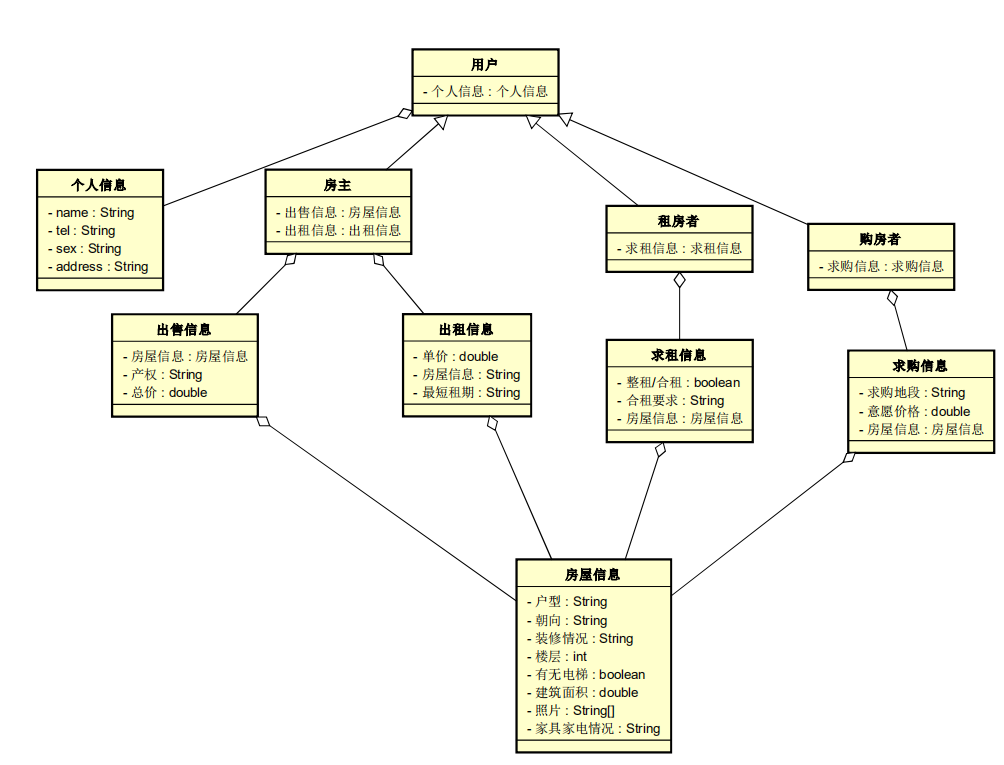
\includegraphics[height=14.0cm,width=14.0cm]{requirement/figures/lingyu.png}%fig2文件夹下的xbee.esp图片,
    
    \caption{顶层架构图}
    
    \end{figure}
	\chapter{小程序测试}

\section{登录功能测试}

功能描述:用户通过微信授权上传昵称和头像并登录到系统

用户操作:在“我的”页面下 点击授权登录

预期结果:后端返回请求数据(url、introduce、message、moblie、name、sex)服务器状态(result、message)字段信息.原“请授权登录”处显示用户的头像、昵称

测试结果:通过
\begin{figure}[htbp]
    \centering
    \begin{minipage}[t]{0.32\textwidth}
    \centering
    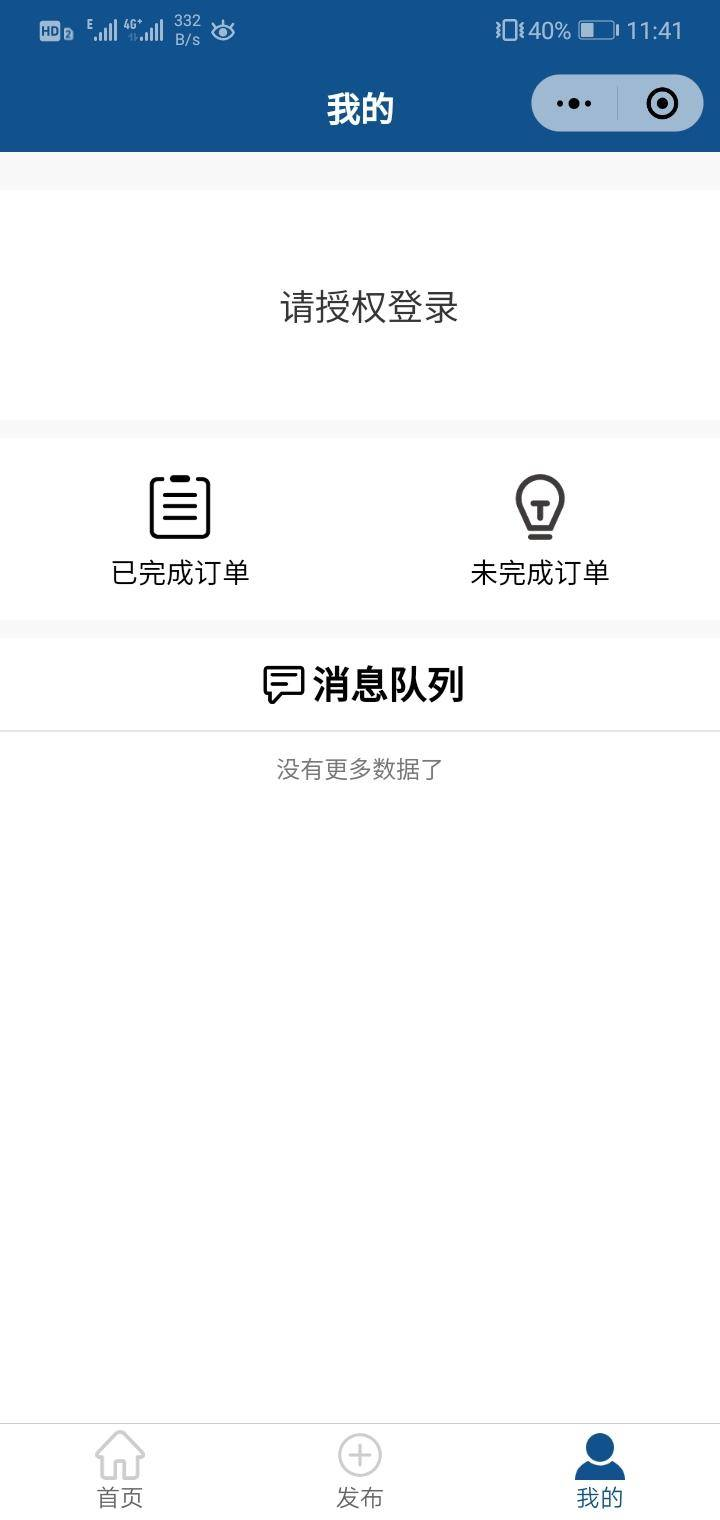
\includegraphics[width=3.8cm,height=8cm]{test/image/test1.png} 
    \caption{登录功能测试1}
    \end{minipage}
    \begin{minipage}[t]{0.32\textwidth}
    \centering
    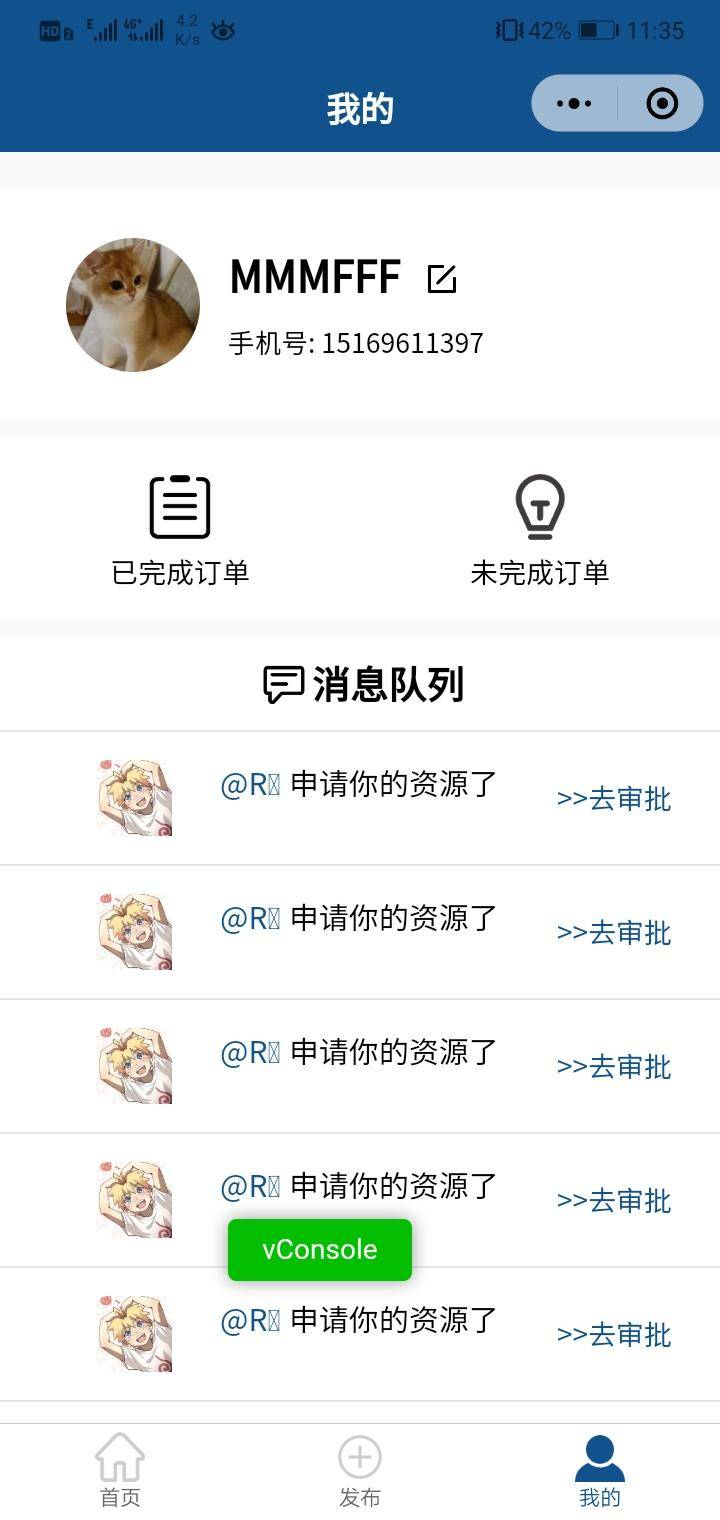
\includegraphics[width=3.8cm,height=8cm]{test/image/test2.png}
    \caption{登录功能测试2}
    \end{minipage}
    \begin{minipage}[t]{0.32\textwidth}
        \centering
        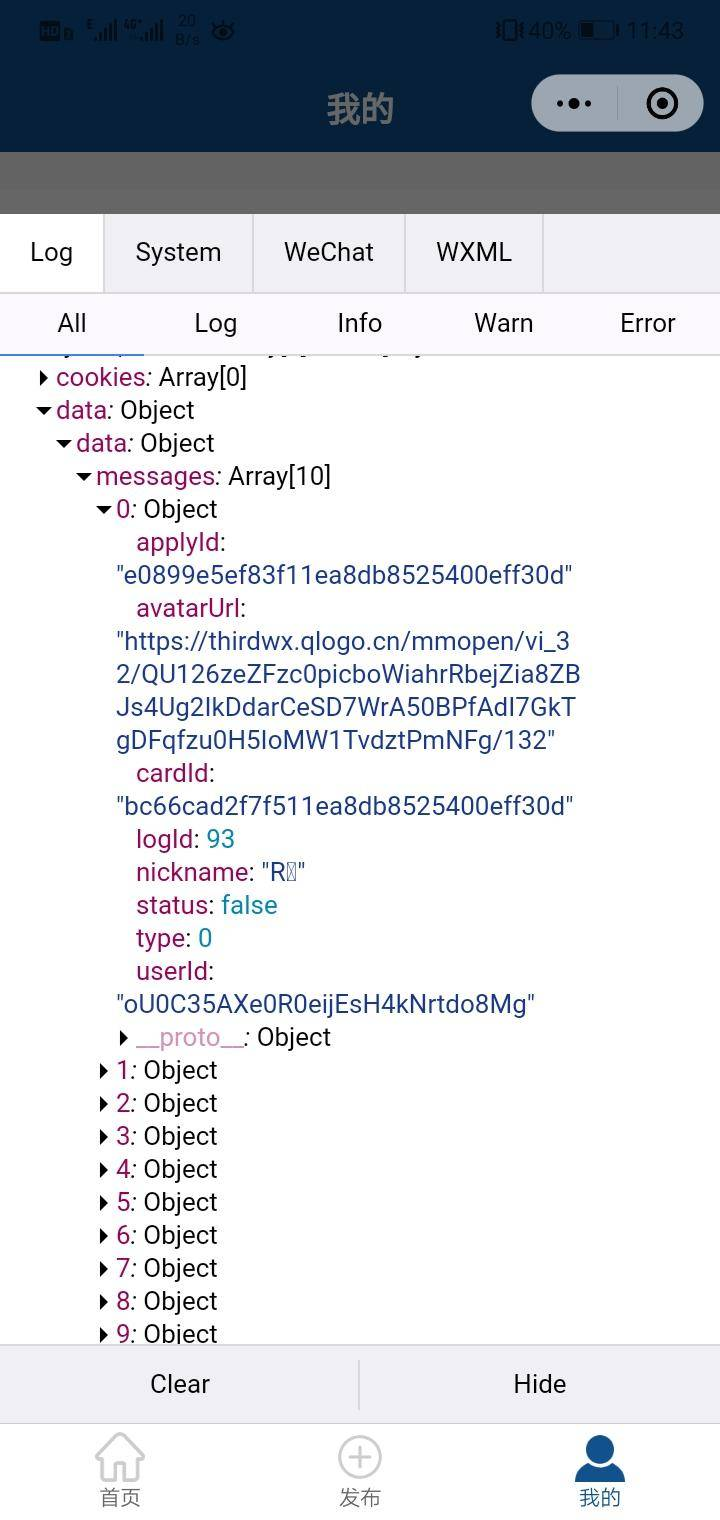
\includegraphics[width=3.8cm,height=8cm]{test/image/test3.png}
        \caption{测试结果}
        \end{minipage}
    \end{figure}

\section{通过手机号获取验证码功能测试}

功能描述:用户输入手机号,发送给服务器用于服务器发送验证码

用户操作:在“手机验证”界面下输入手机号点击获取验证码

预期结果:通过短信收到验证码,服务器返回状态码(result、message)

测试结果:通过

\newpage
\begin{figure}[htbp]
    \centering
    \begin{minipage}[t]{0.48\textwidth}
    \centering
    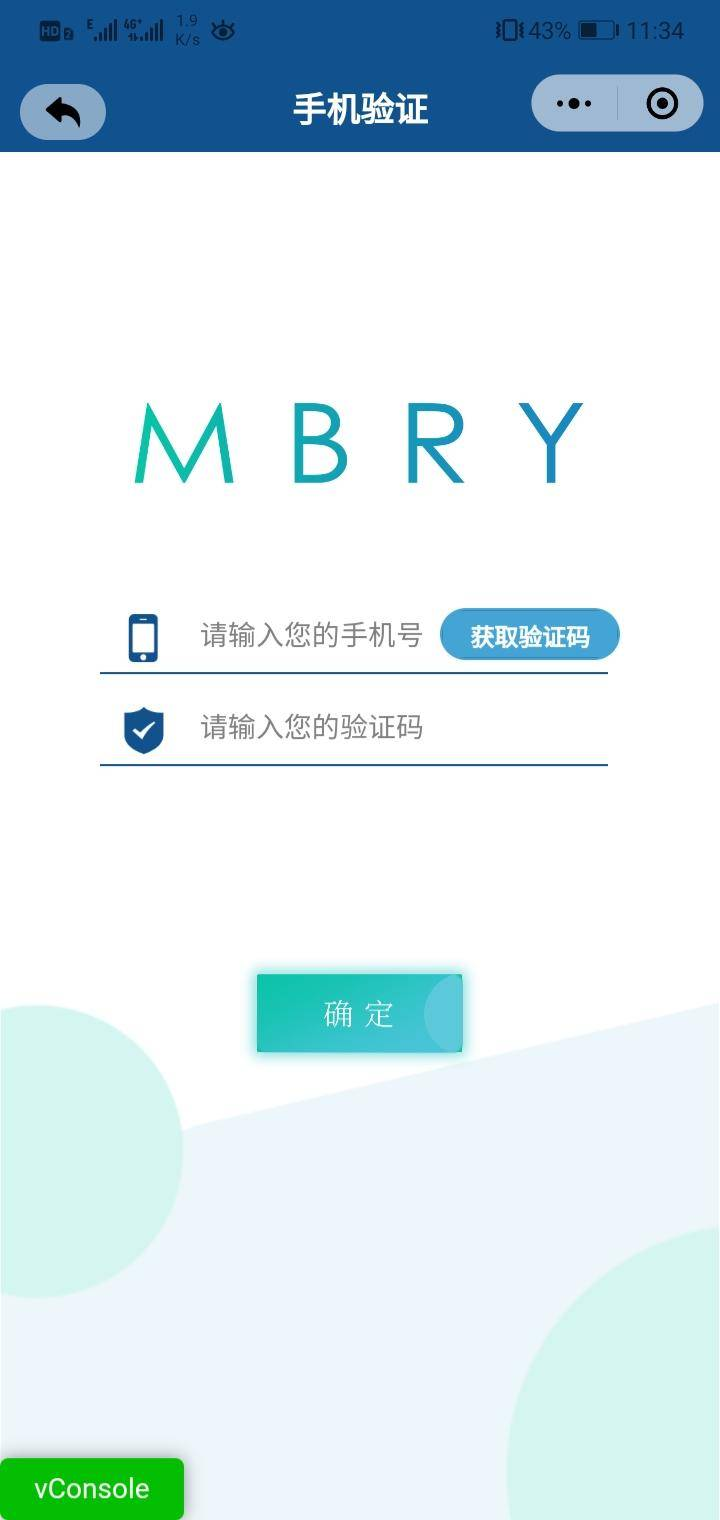
\includegraphics[width=4cm,height=8cm]{test/image/test4.png} 
    \caption{获取验证码}
    \end{minipage}
    \end{figure}
 
\section{绑定手机号功能测试}
功能描述:用户输入手机号验证码,绑定手机号

用户操作:在3.2基础上输入验证码

预期结果:页面跳转、提示绑定成功

测试结果:通过

\begin{figure}[htbp]
    \centering
    \begin{minipage}[t]{0.48\textwidth}
    \centering
    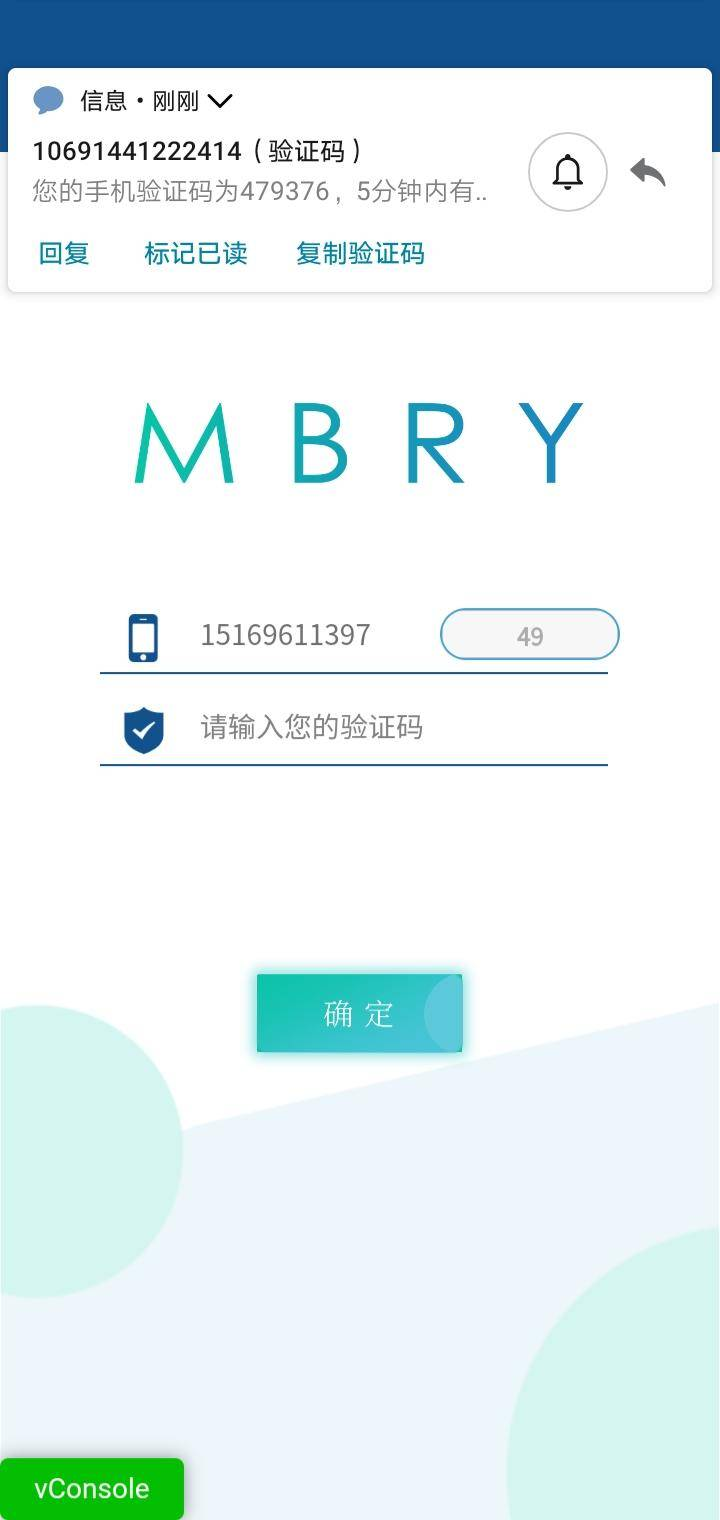
\includegraphics[width=4cm,height=8cm]{test/image/test5.png} 
    \caption{输入验证码}
    \end{minipage}
\end{figure}
\newpage

\section{浏览最新帖子功能测试}
实现用例1:房屋信息查询

功能描述:用户可在首页查看最新发布的帖子

用户操作:在“首页”页面下,用户可查看帖子列表。

预期结果:服务器返回帖子数据;在首页下半部分会按发布时间顺序展示最新发布的帖子,帖子列表可下拉

测试结果:通过

\begin{figure}[htbp]
    \centering
    \begin{minipage}[t]{0.48\textwidth}
    \centering
    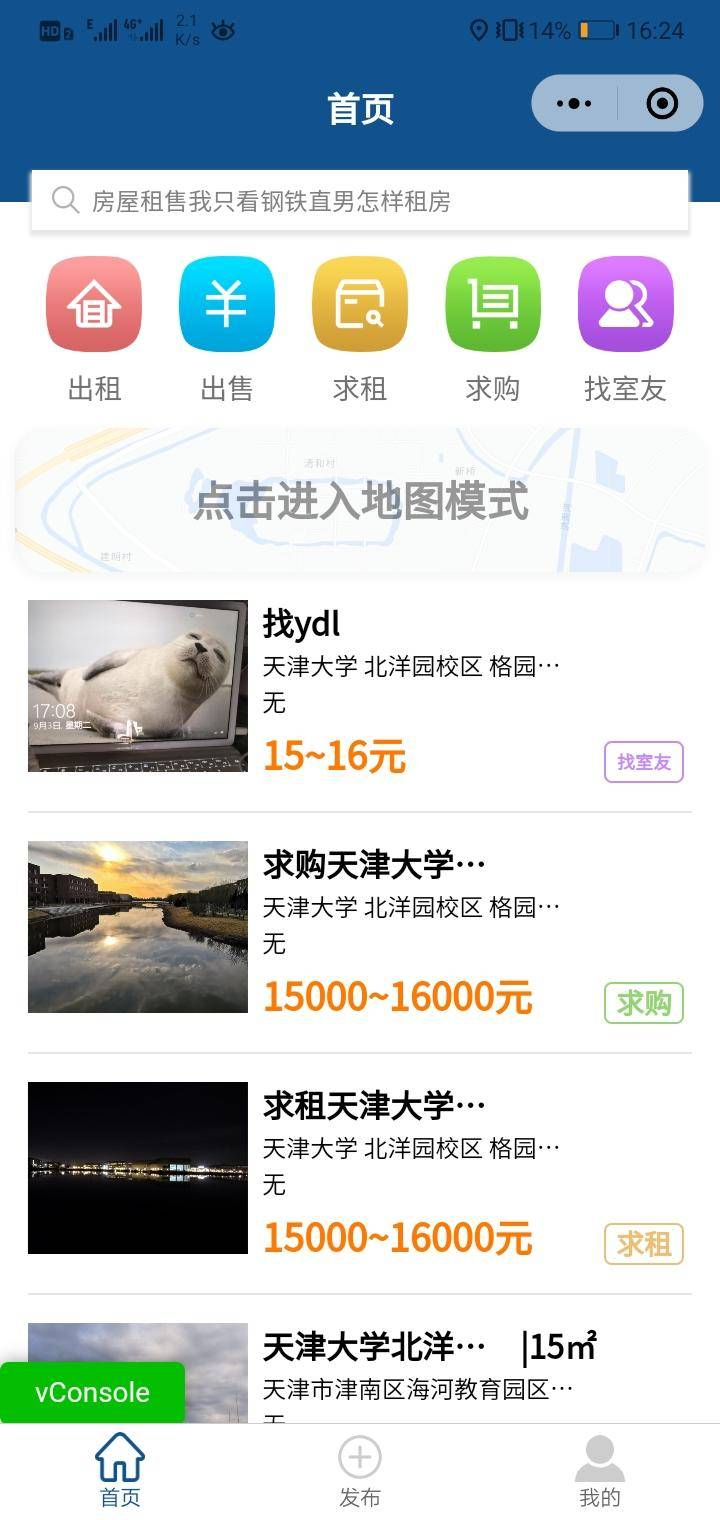
\includegraphics[width=4cm,height=8cm]{test/image/test6.png} 
    \caption{首页}
    \end{minipage}
    \begin{minipage}[t]{0.48\textwidth}
    \centering
    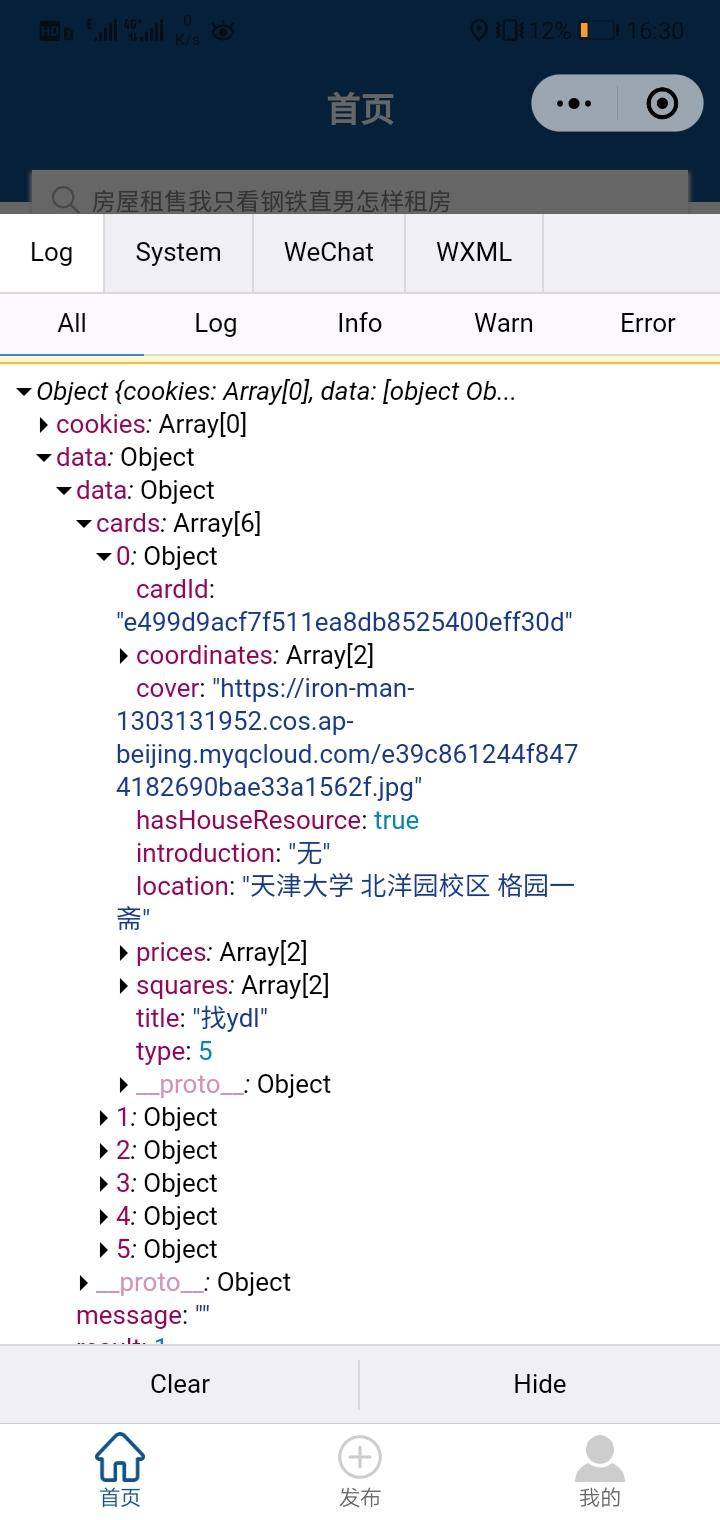
\includegraphics[width=4cm,height=8cm]{test/image/test7.png}
    \caption{测试结果}
    \end{minipage}
    \end{figure}
\section{查看出租帖子功能测试}
实现用例1:房屋信息查询

功能描述:用户可指定查看出租类型的帖子

用户操作:在“首页”页面下,点击出租 

预期结果:服务器返回出租帖子数据,进入出租帖子查询界面

测试结果:通过
\newpage

\begin{figure}[htbp]
    \centering
    \begin{minipage}[t]{0.32\textwidth}
        \centering
        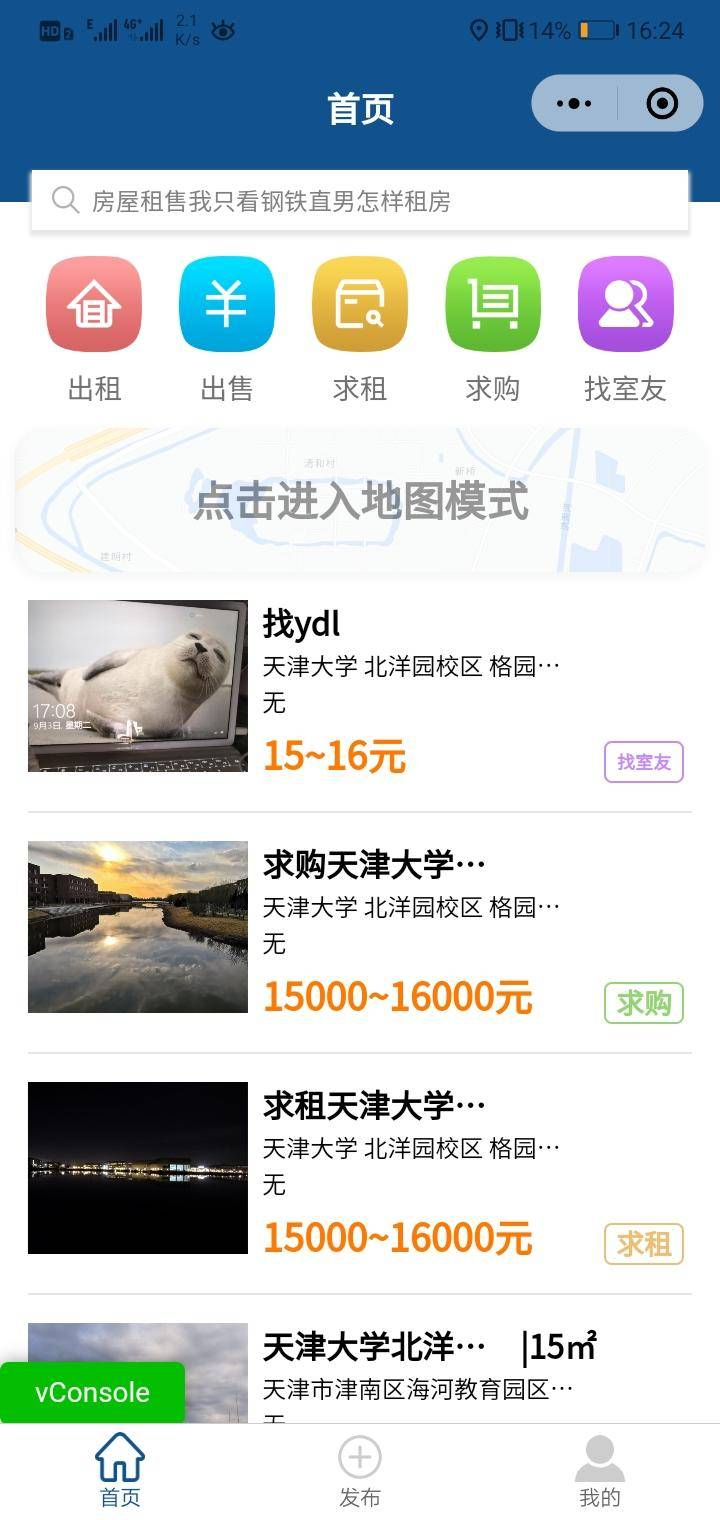
\includegraphics[width=3.8cm,height=8cm]{test/image/test8.png} 
       \caption{出租界面} 
        \end{minipage}
    \begin{minipage}[t]{0.32\textwidth}
    \centering
    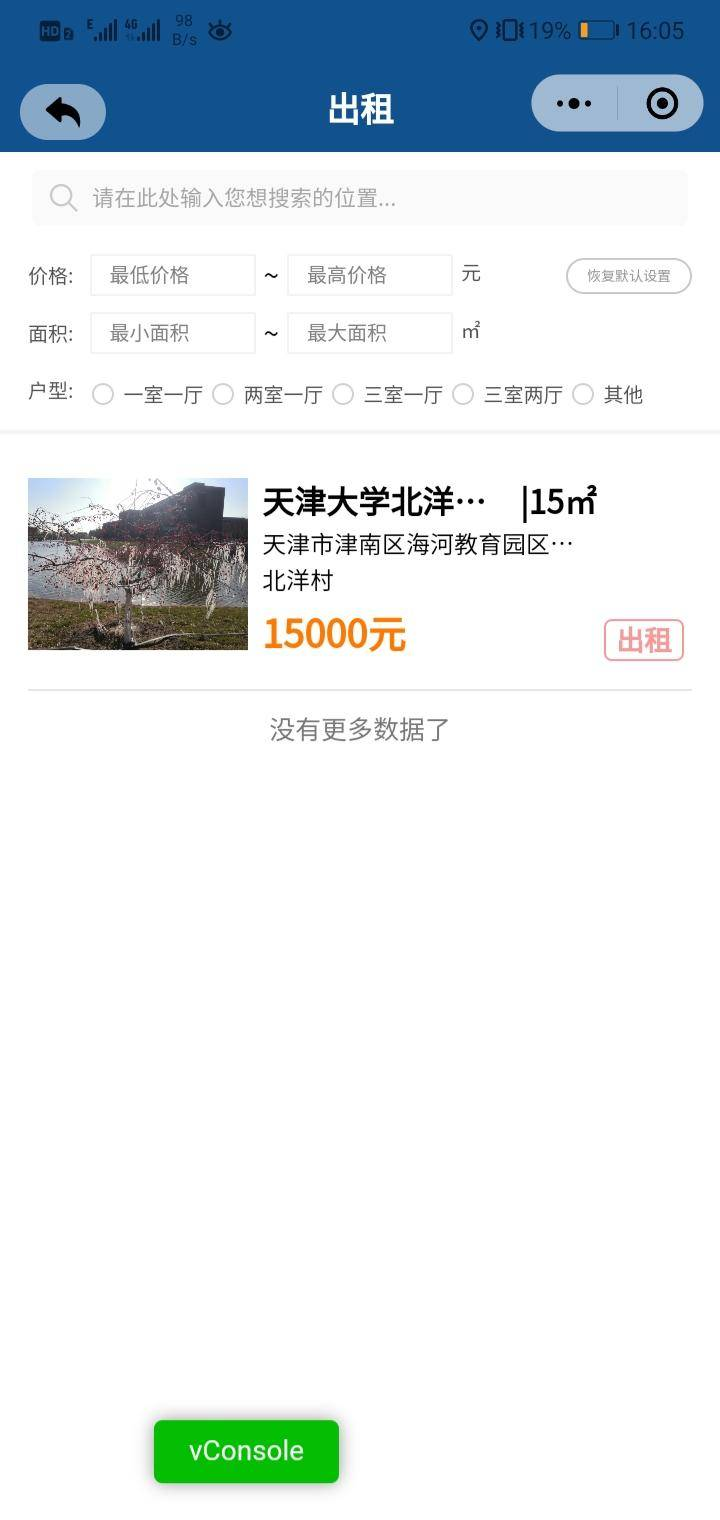
\includegraphics[width=3.8cm,height=8cm]{test/image/test9.png} 
   \caption{出租界面} 
    \end{minipage}
    \begin{minipage}[t]{0.32\textwidth}
    \centering
    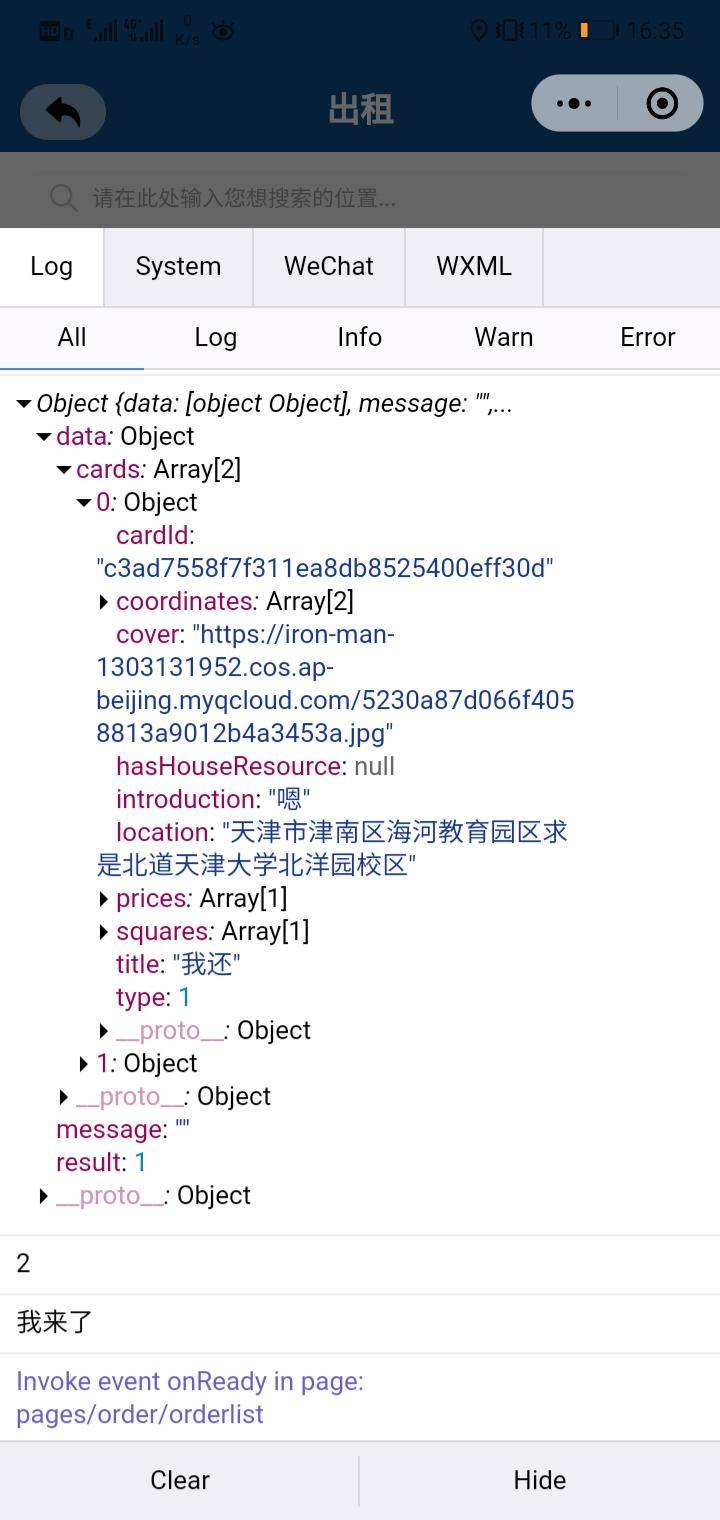
\includegraphics[width=3.8cm,height=8cm]{test/image/test10.png}
    \caption{测试结果}
    \end{minipage}
    \end{figure}

\section{查看出售帖子功能测试}
实现用例1:房屋信息查询

功能描述:用户可指定查看出售类型的帖子

用户操作:在“首页”页面下,点击出售

预期结果:服务器返回出售帖子数据,进入出售帖子查询界面

测试结果:通过

\begin{figure}[htbp]
    \centering
    \begin{minipage}[t]{0.32\textwidth}
        \centering
        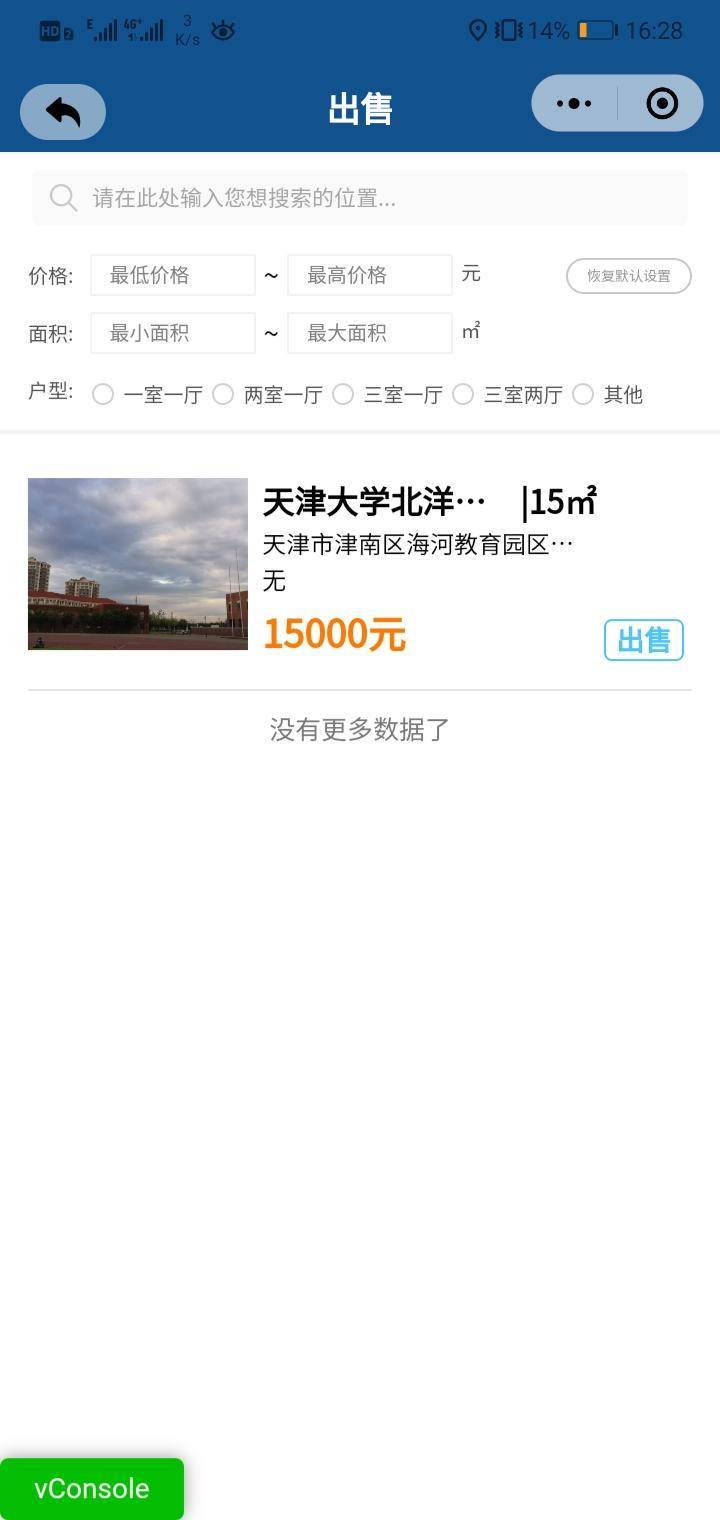
\includegraphics[width=3.8cm,height=8cm]{test/image/test11.png} 
       \caption{出售界面} 
        \end{minipage}
    \begin{minipage}[t]{0.32\textwidth}
    \centering
    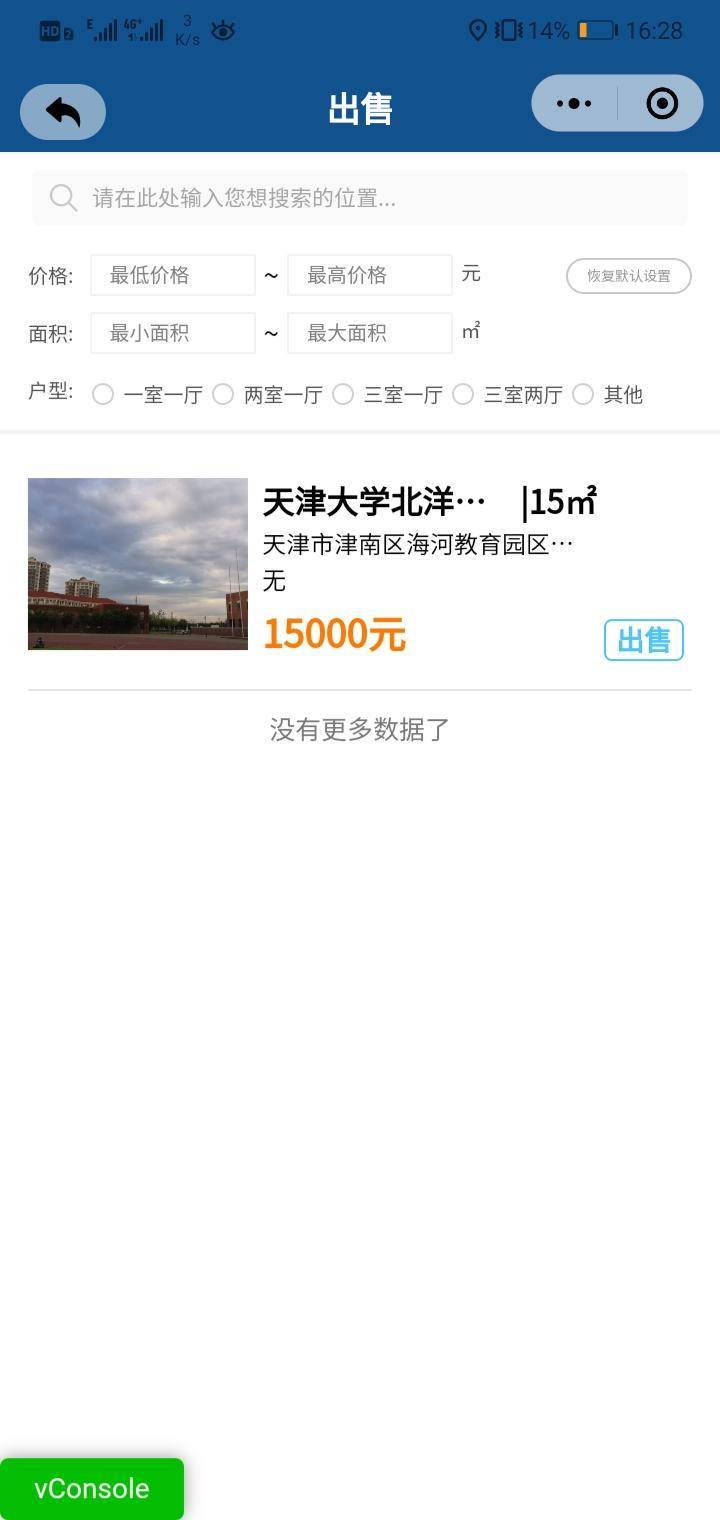
\includegraphics[width=3.8cm,height=8cm]{test/image/test11.png} 
   \caption{出售界面} 
    \end{minipage}
    \begin{minipage}[t]{0.32\textwidth}
    \centering
    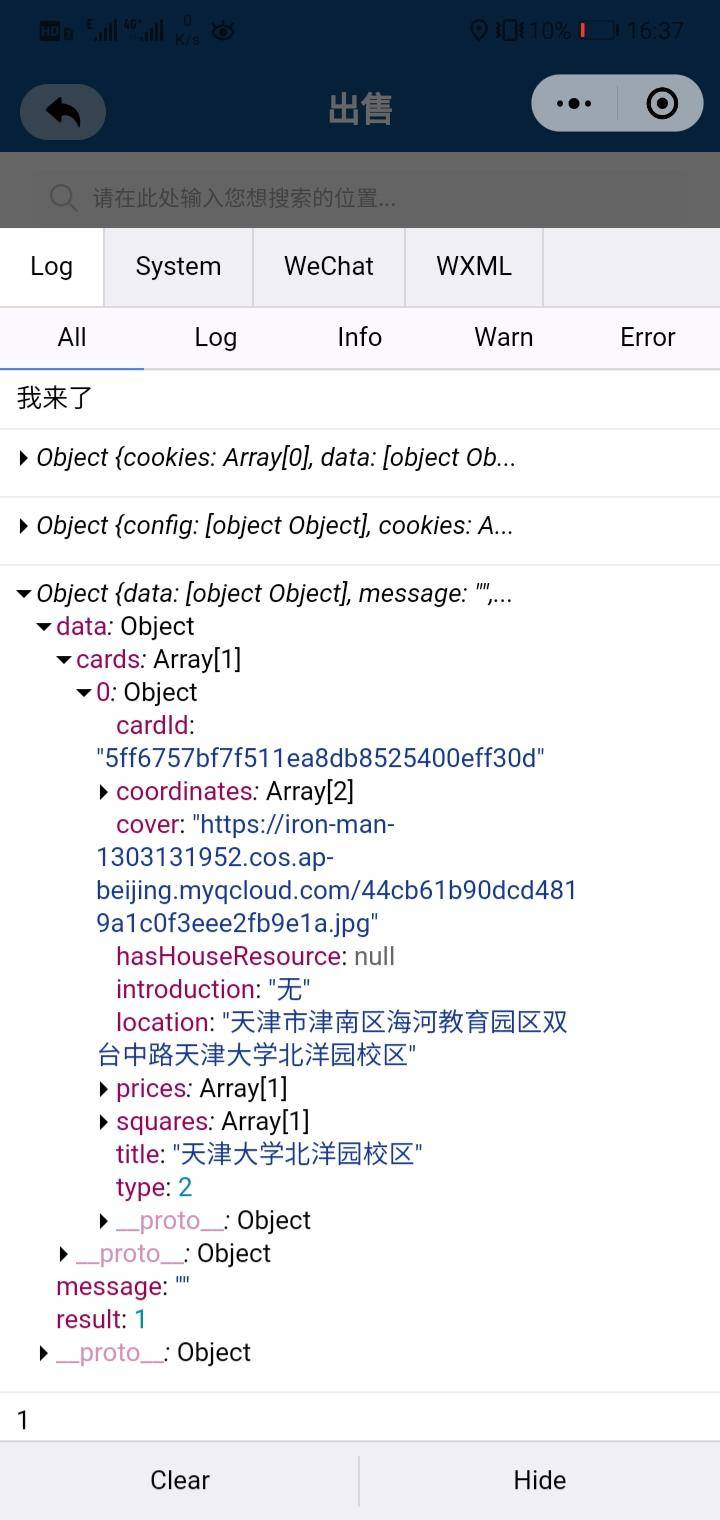
\includegraphics[width=3.8cm,height=8cm]{test/image/test12.png}
    \caption{测试结果}
    \end{minipage}
    \end{figure}
 
\section{查看求租帖子功能测试}
实现用例1:房屋信息查询

功能描述:用户可指定查看求租类型的帖子

用户操作:在“首页”页面下,点击求租

预期结果:服务器返回求租帖子数据,进入求租帖子查询界面

测试结果:通过
\begin{figure}[htbp]
    \centering
    \begin{minipage}[t]{0.32\textwidth}
        \centering
        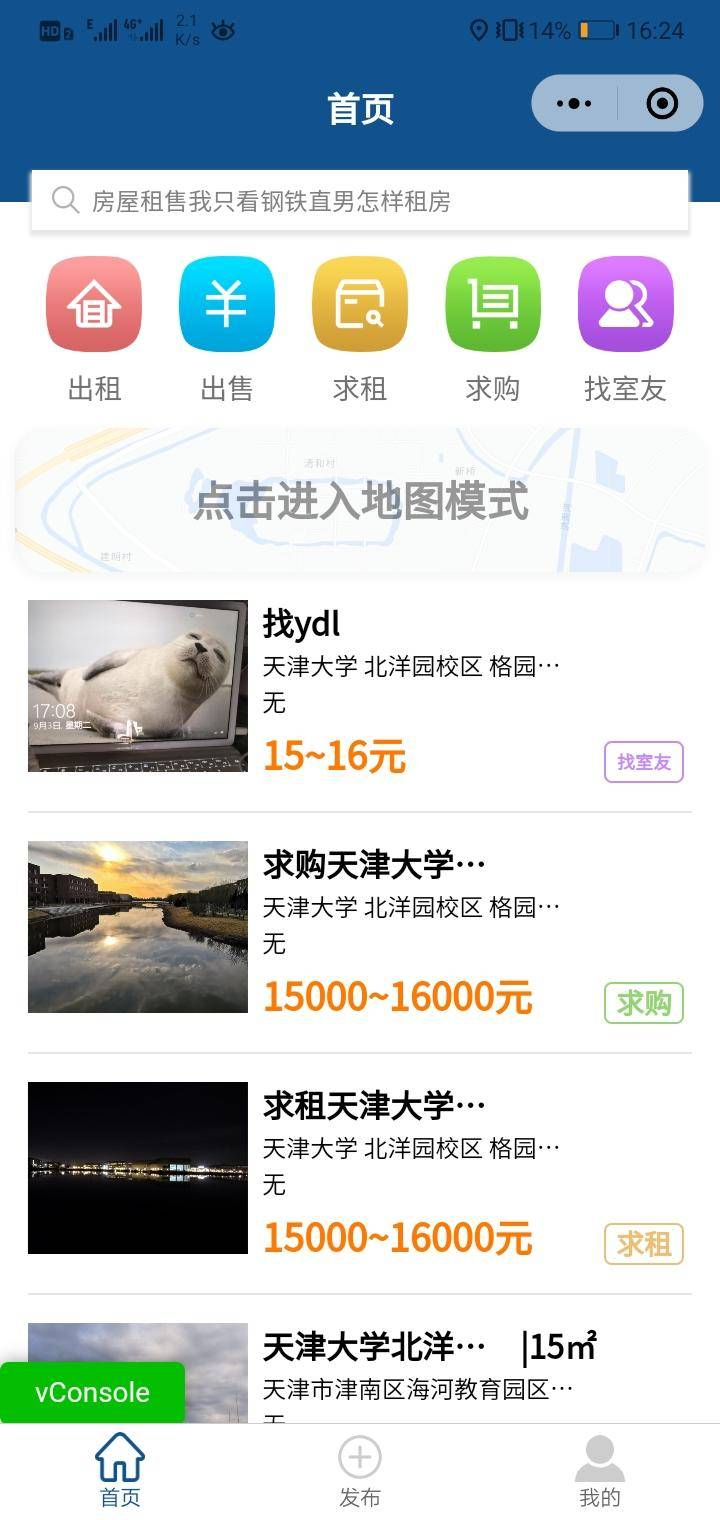
\includegraphics[width=3.8cm,height=8cm]{test/image/test13.png} 
       \caption{求租界面} 
        \end{minipage}
    \begin{minipage}[t]{0.32\textwidth}
    \centering
    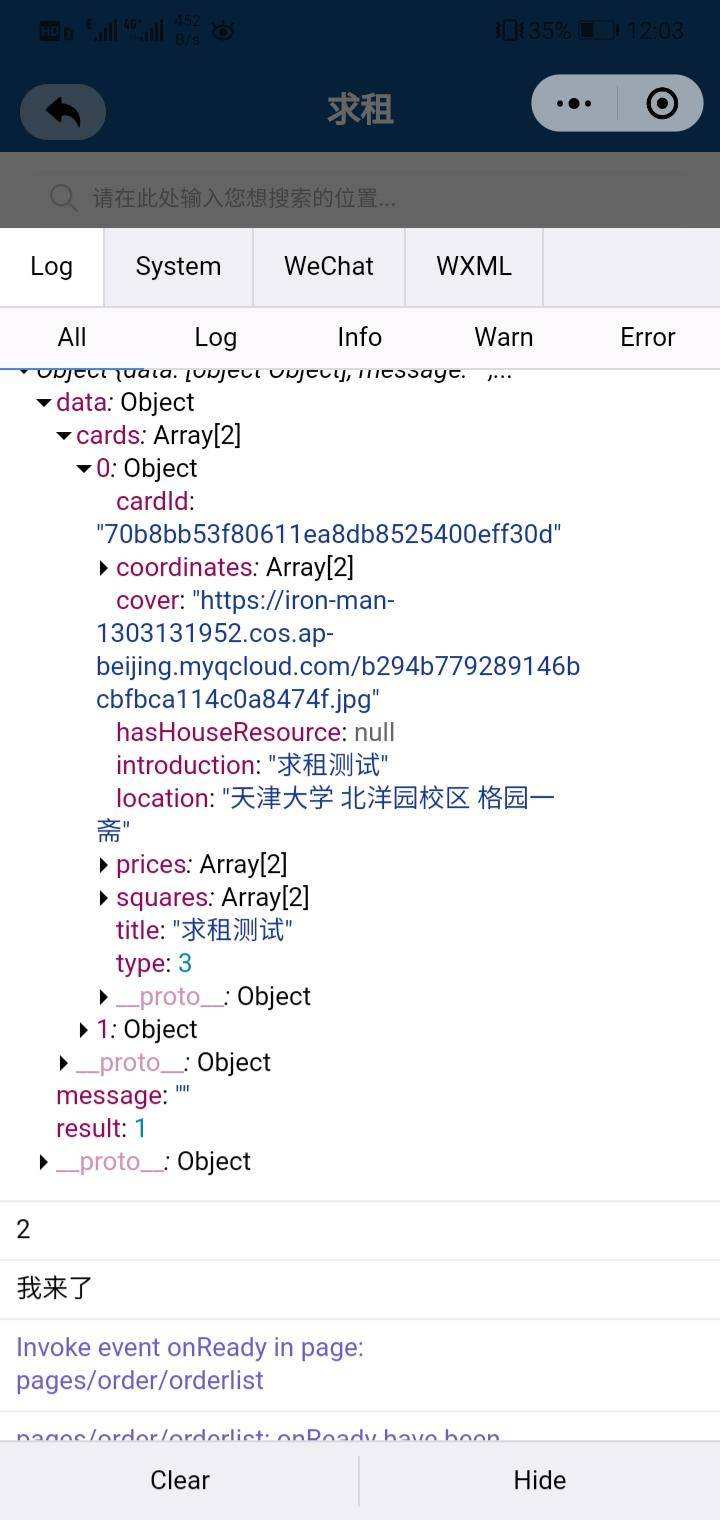
\includegraphics[width=3.8cm,height=8cm]{test/image/test14.png} 
   \caption{求租界面} 
    \end{minipage}
    \begin{minipage}[t]{0.32\textwidth}
    \centering
    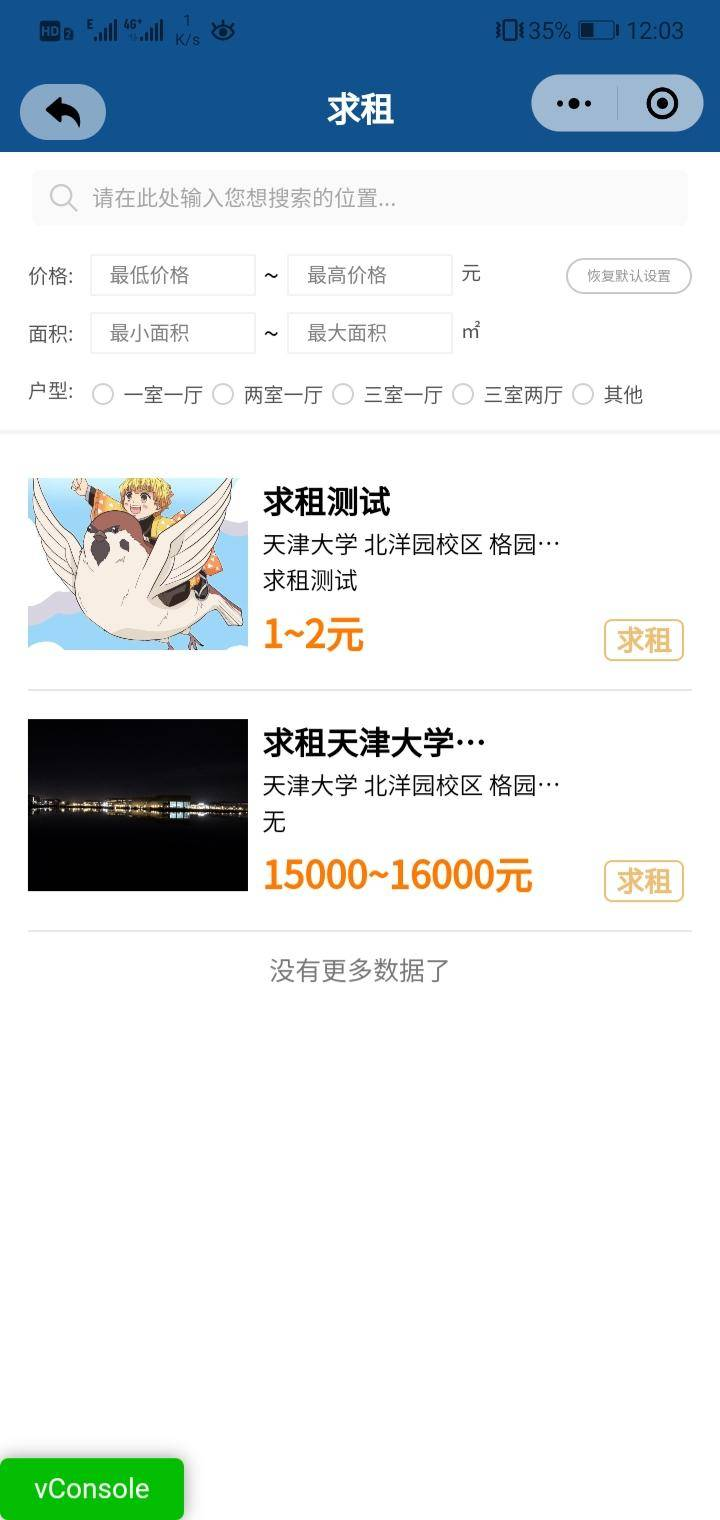
\includegraphics[width=3.8cm,height=8cm]{test/image/test15.png}
    \caption{测试结果}
    \end{minipage}
    \end{figure}
  
\section{查看求购帖子功能测试}
实现用例1:房屋信息查询

功能描述:用户可指定查看求售类型的帖子

用户操作:在“首页”页面下,点击求售

预期结果:服务器返回求售帖子数据,进入求售帖子查询界面

测试结果:通过
\newpage
\begin{figure}[htbp]
    \centering
    \begin{minipage}[t]{0.32\textwidth}
        \centering
        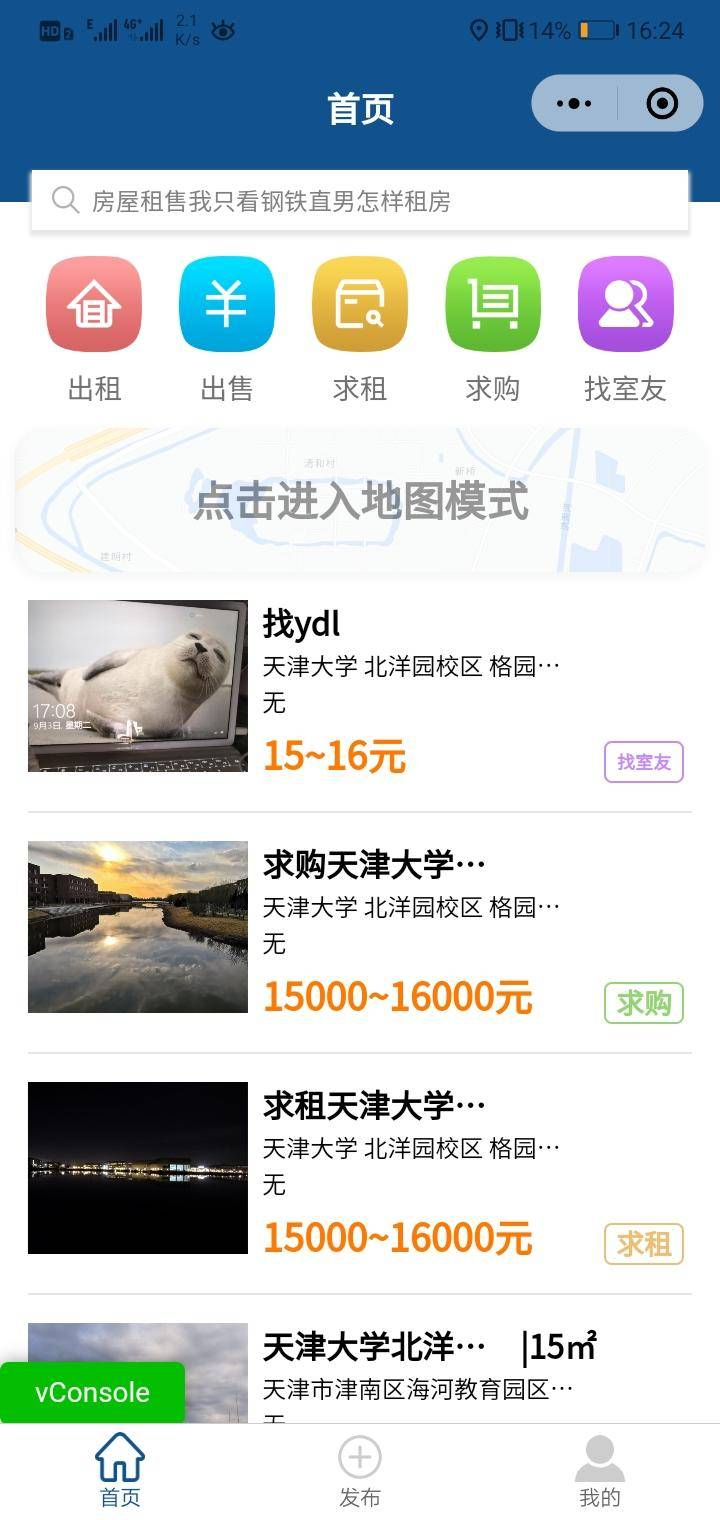
\includegraphics[width=3.8cm,height=8cm]{test/image/test13.png} 
       \caption{求购界面} 
        \end{minipage}
    \begin{minipage}[t]{0.32\textwidth}
    \centering
    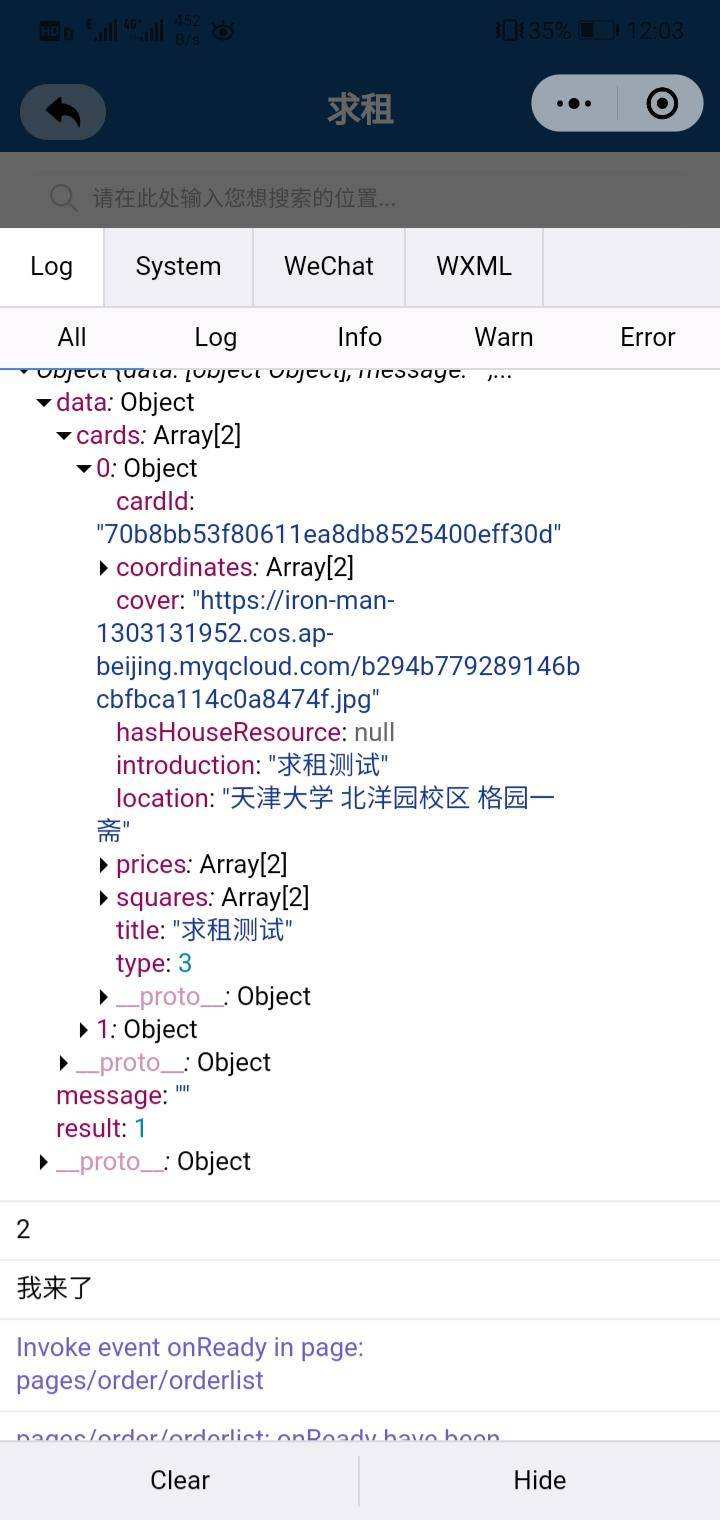
\includegraphics[width=3.8cm,height=8cm]{test/image/test14.png} 
   \caption{求购界面} 
    \end{minipage}
    \begin{minipage}[t]{0.32\textwidth}
    \centering
    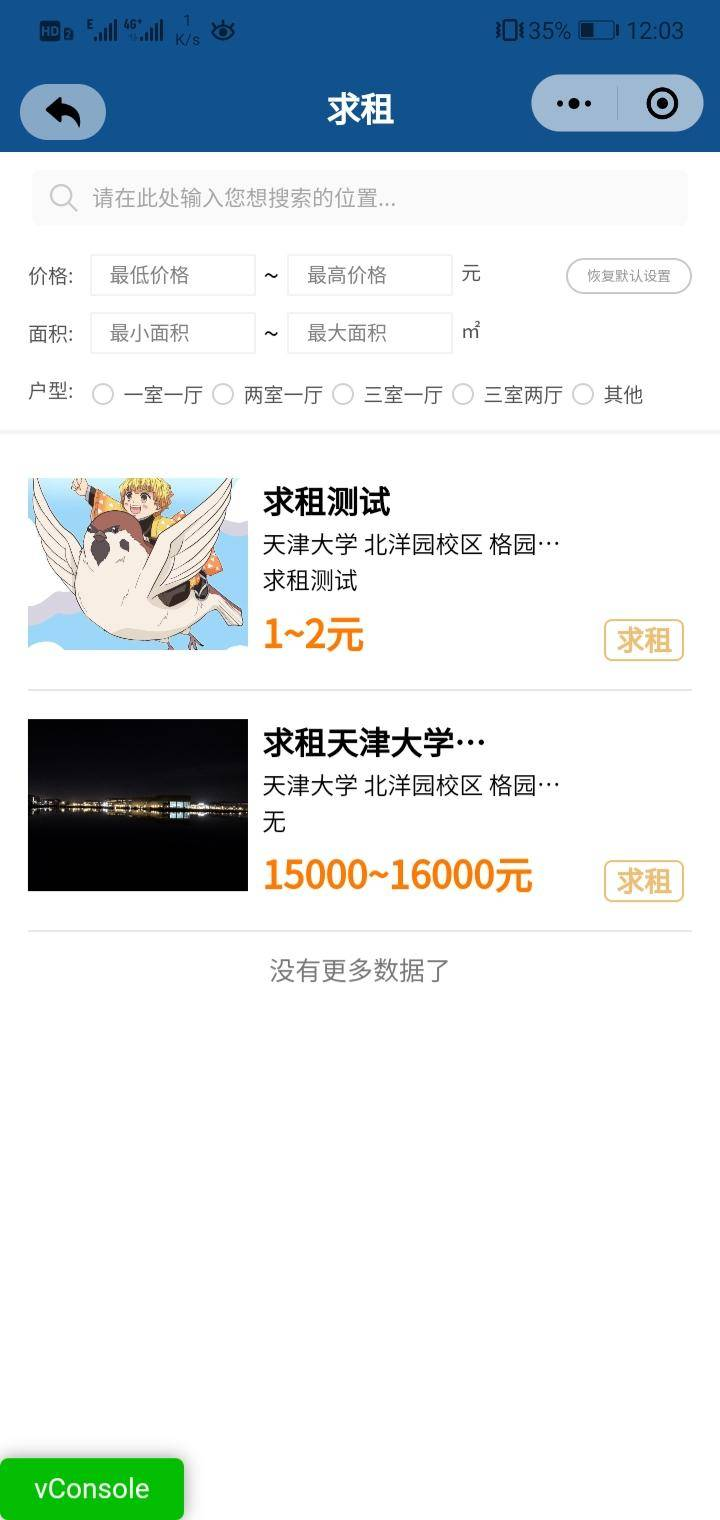
\includegraphics[width=3.8cm,height=8cm]{test/image/test15.png}
    \caption{测试结果}
    \end{minipage}
    \end{figure}

\section{查看求租找室友帖子功能测试}
实现用例1:房屋信息查询

功能描述:用户可指定查看找室友类型的帖子

用户操作:在“首页”页面下,点击找室友

预期结果:服务器返回找室友帖子数据,进入找室友帖子查询界面

测试结果:通过
\begin{figure}[htbp]
    \centering
    \begin{minipage}[t]{0.32\textwidth}
        \centering
        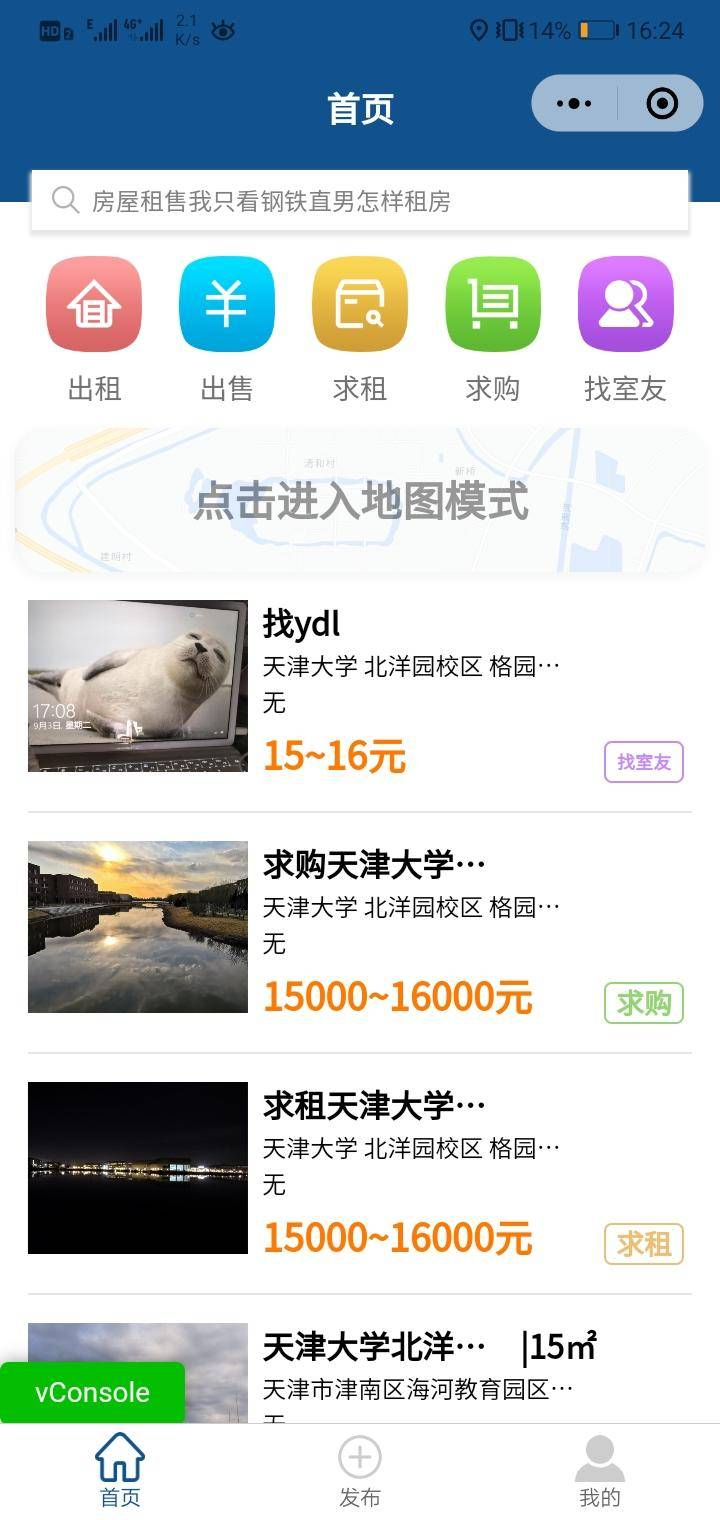
\includegraphics[width=3.8cm,height=8cm]{test/image/test16.png} 
       \caption{找室友界面} 
        \end{minipage}
    \begin{minipage}[t]{0.32\textwidth}
    \centering
    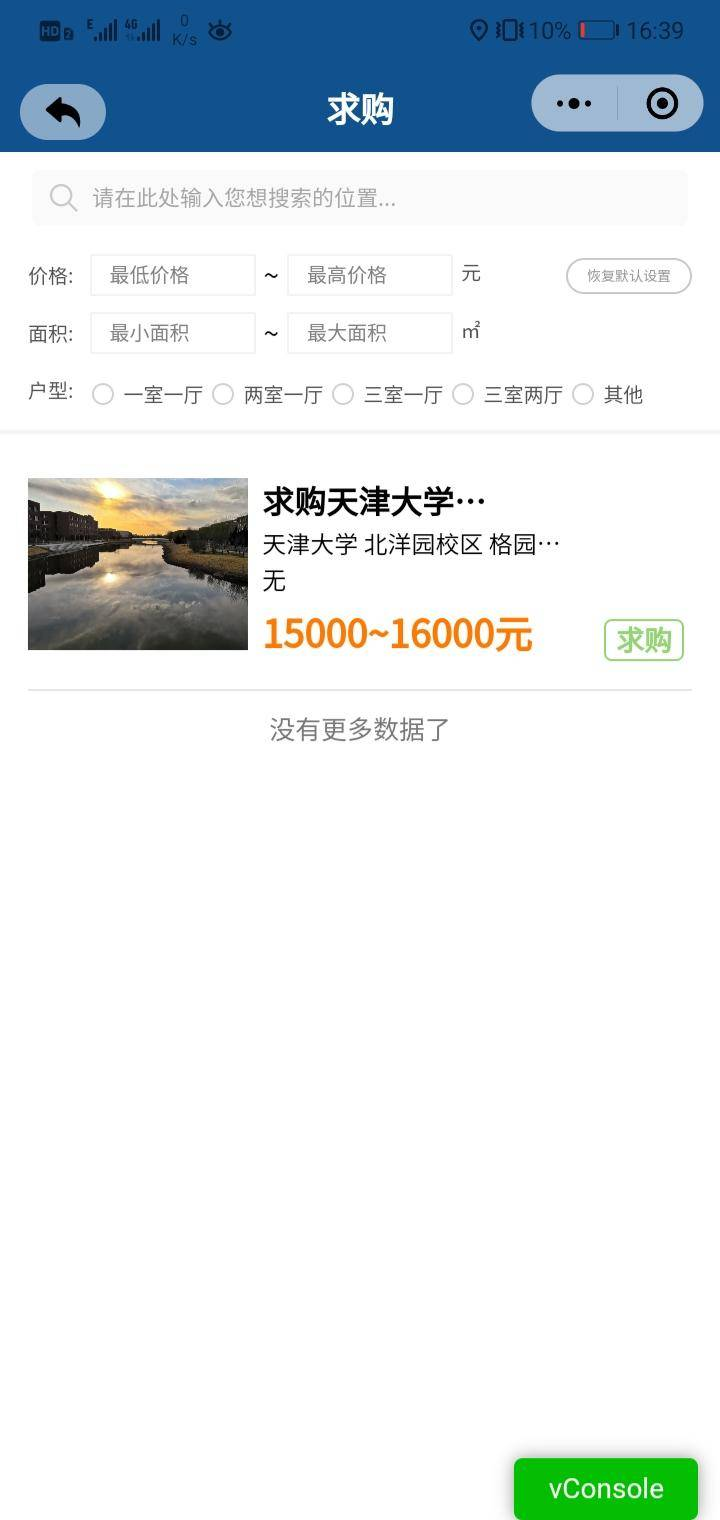
\includegraphics[width=3.8cm,height=8cm]{test/image/test17.png} 
   \caption{找室友界面} 
    \end{minipage}
    \begin{minipage}[t]{0.32\textwidth}
    \centering
    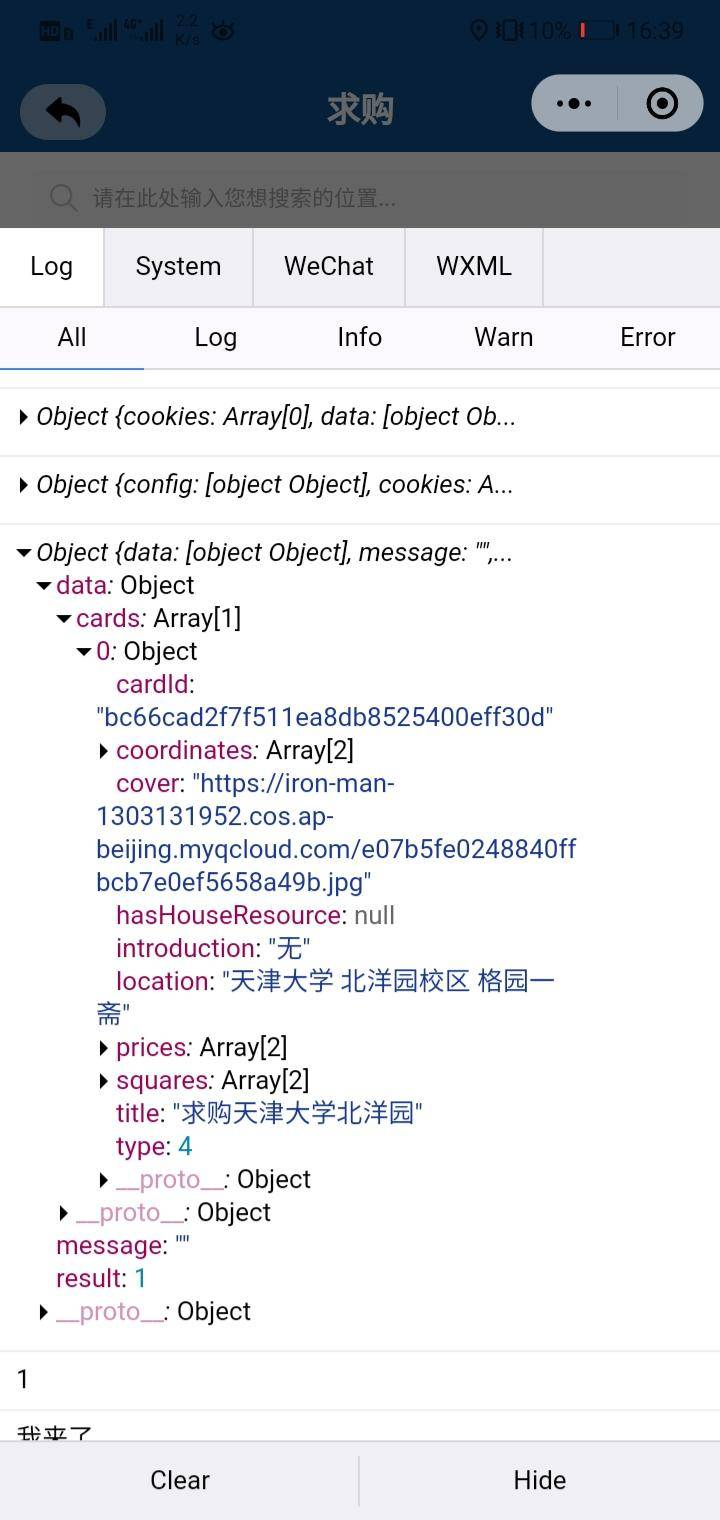
\includegraphics[width=3.8cm,height=8cm]{test/image/test18.png}
    \caption{测试结果}
    \end{minipage}
    \end{figure}
   \newpage 

\section{搜索帖子功能测试}

实现用例1:房屋信息查询

功能描述:用户可以通过地区字段搜索相关的帖子

用户操作:在“搜索“界面 选择帖子类型 输入地区字段 点击搜索

预期结果:服务器返回找室友帖子数据,进入找室友帖子查询界面

测试结果:通过
\begin{figure}[htbp]
    \centering
    \begin{minipage}[t]{0.32\textwidth}
        \centering
        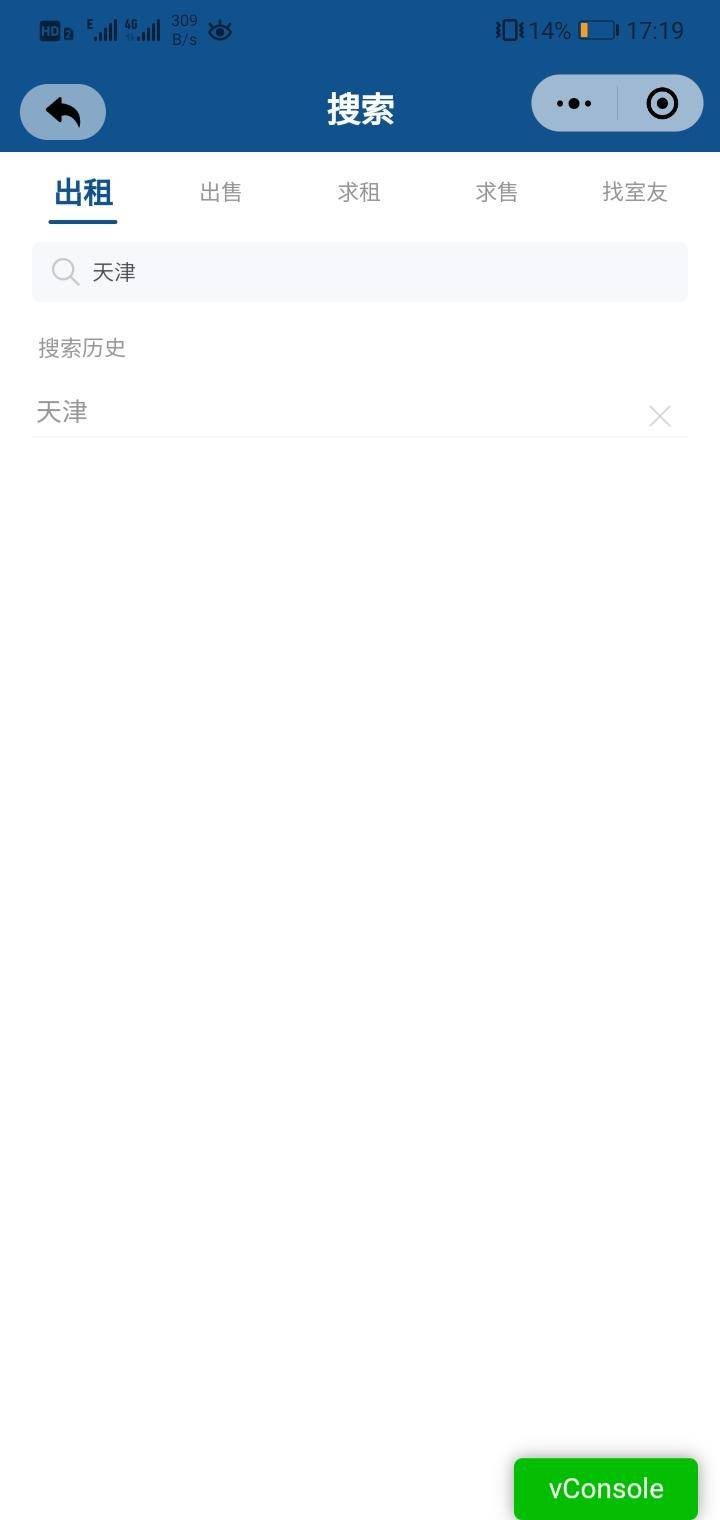
\includegraphics[width=3.8cm,height=8cm]{test/image/test19.png} 
       \caption{搜索界面} 
        \end{minipage}
    \begin{minipage}[t]{0.32\textwidth}
    \centering
    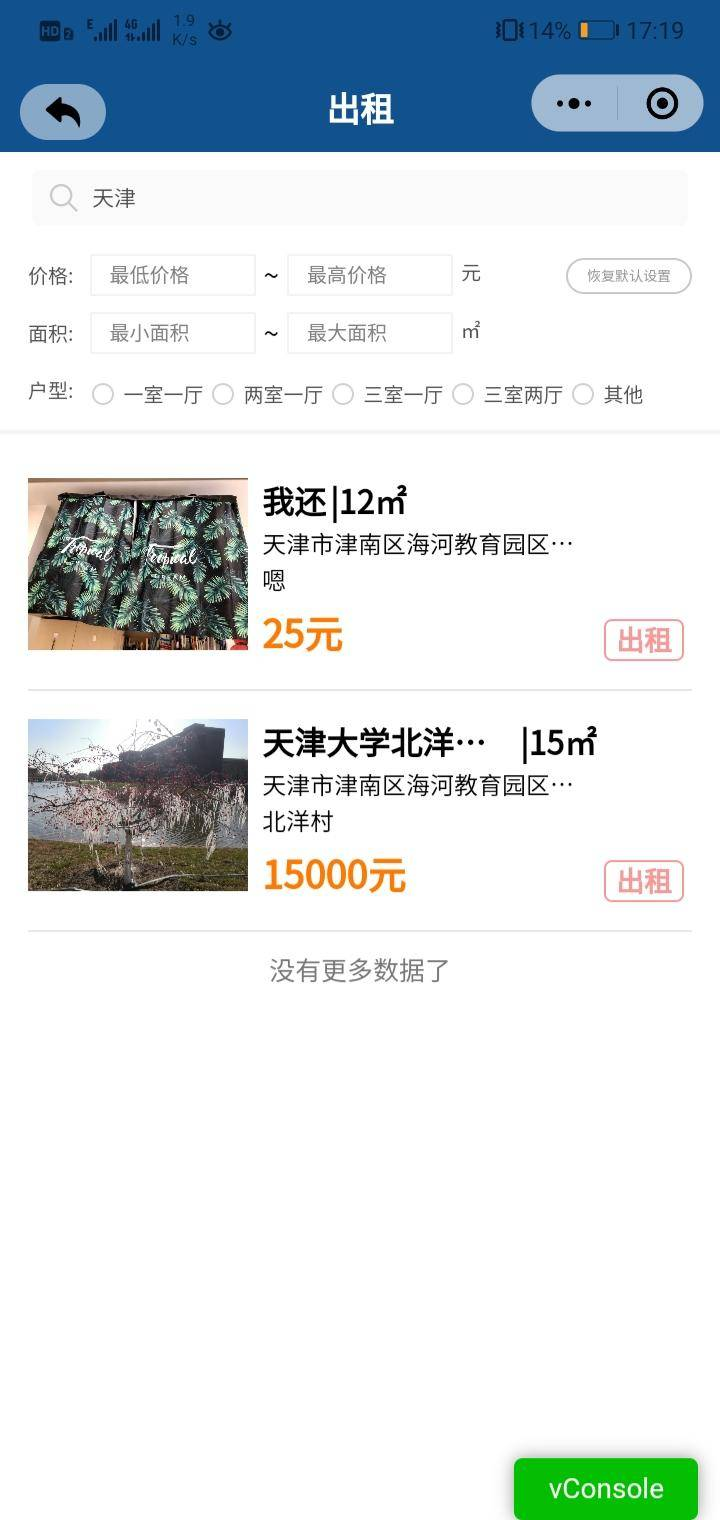
\includegraphics[width=3.8cm,height=8cm]{test/image/test20.png} 
   \caption{搜索结果界面} 
    \end{minipage}
    \begin{minipage}[t]{0.32\textwidth}
    \centering
    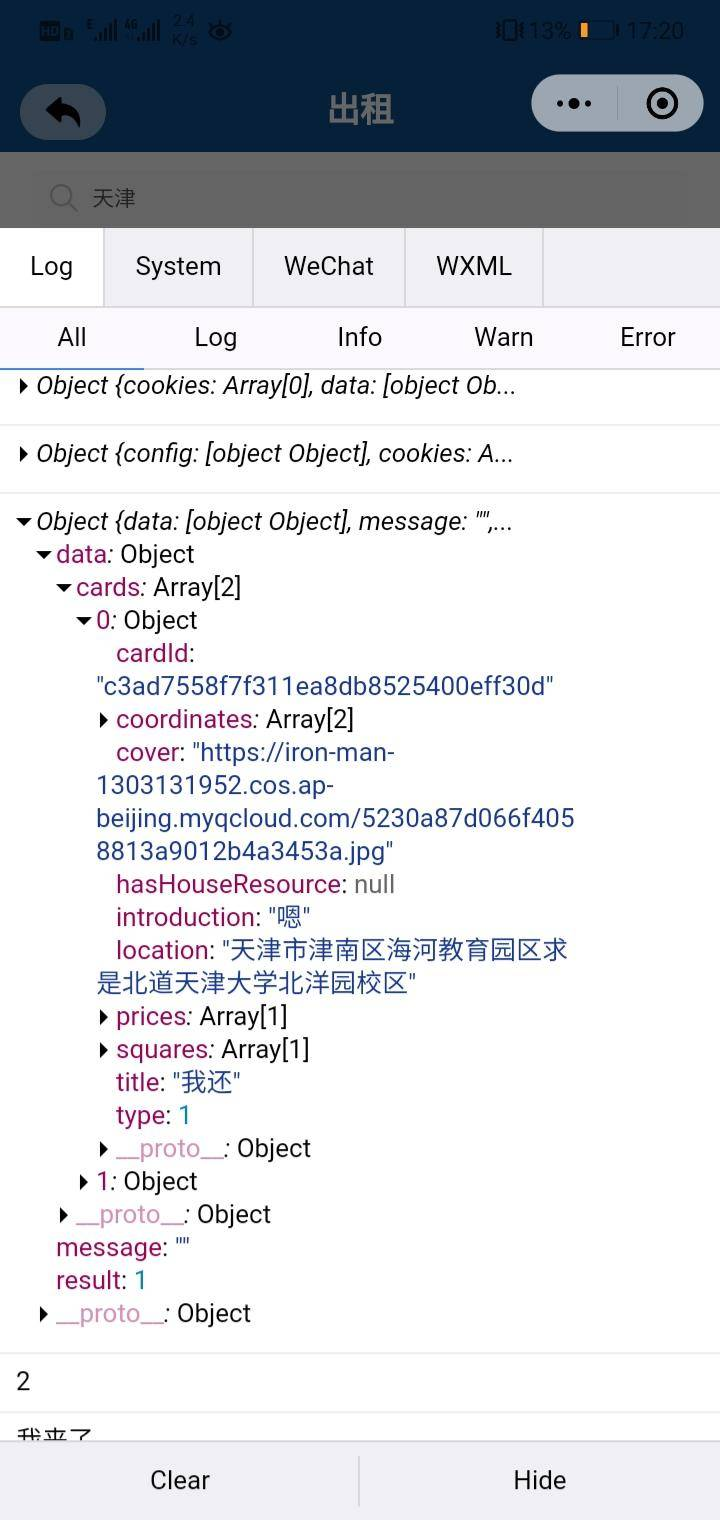
\includegraphics[width=3.8cm,height=8cm]{test/image/test21.png}
    \caption{测试结果}
    \end{minipage}
    \end{figure}

\section{按价格面积户型搜索帖子功能测试}
实现用例1:房屋信息查询

功能描述:用户可以通过价格面积字段搜索相关的帖子

用户操作:在“出租“界面 输入价格区间 面积区间 户型

预期结果:服务器返回指定类型的帖子数据列表展示出符合条件的帖子

测试结果:通过
\newpage
\begin{figure}[htbp]
    \centering
    \begin{minipage}[t]{0.32\textwidth}
        \centering
        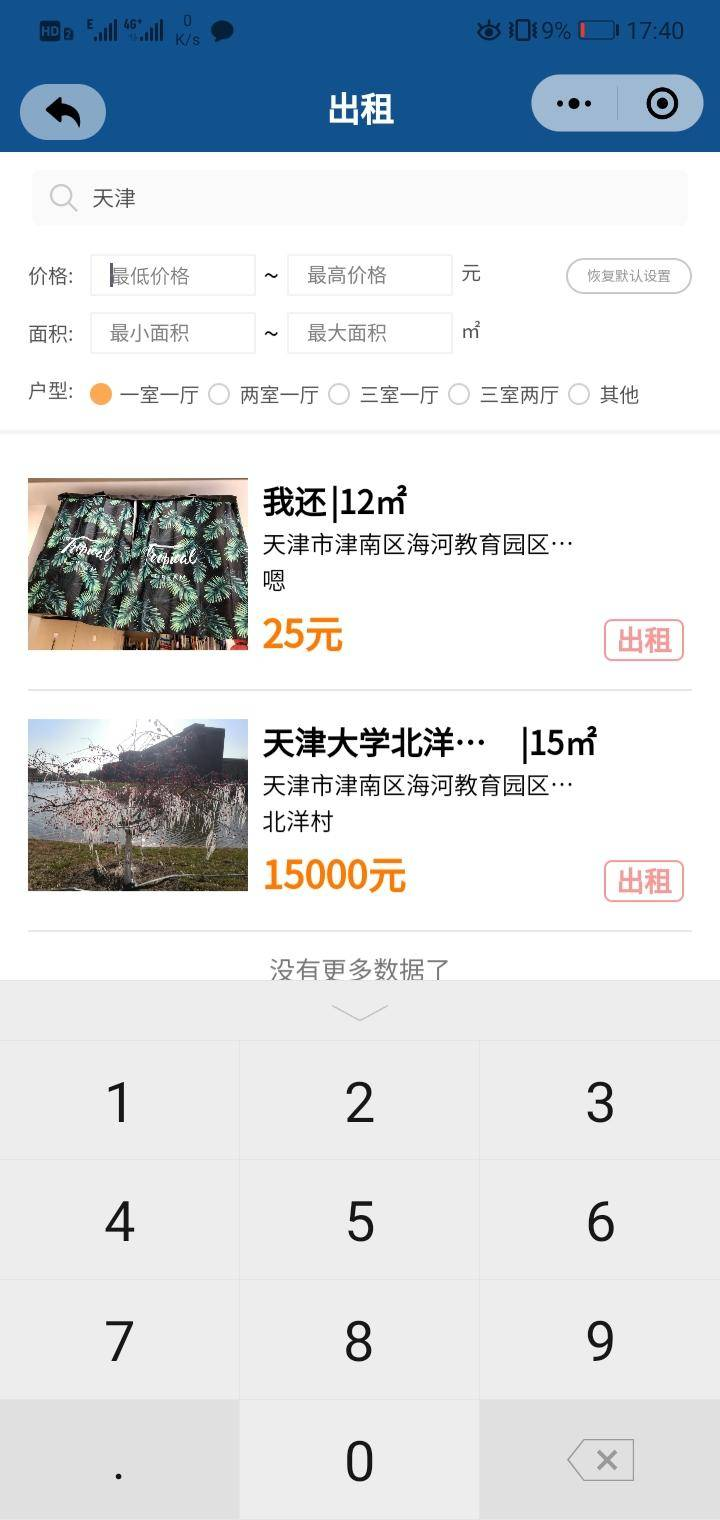
\includegraphics[width=3.8cm,height=8cm]{test/image/test22.png} 
       \caption{输入搜索条件} 
        \end{minipage}
    \begin{minipage}[t]{0.32\textwidth}
    \centering
    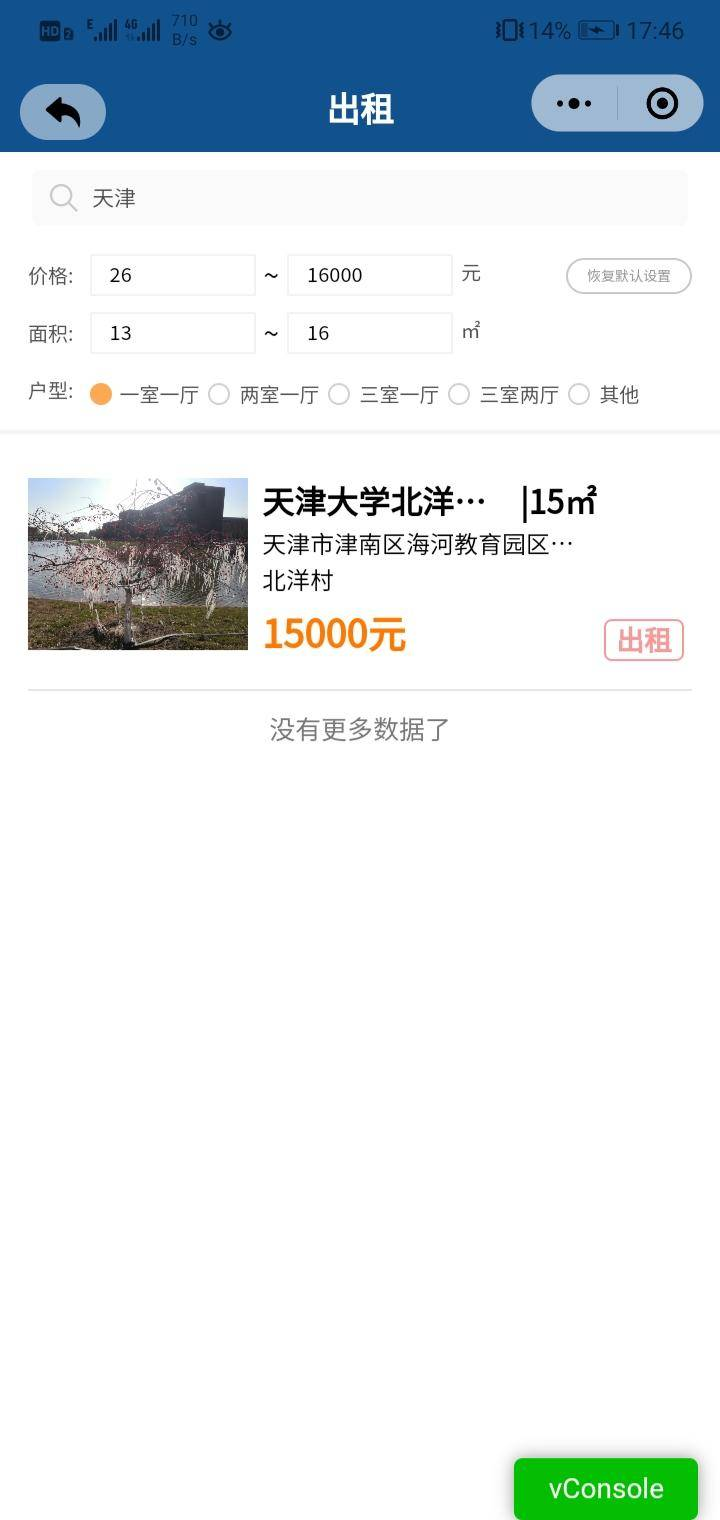
\includegraphics[width=3.8cm,height=8cm]{test/image/test23.png} 
   \caption{搜索结果} 
    \end{minipage}
    \begin{minipage}[t]{0.32\textwidth}
    \centering
    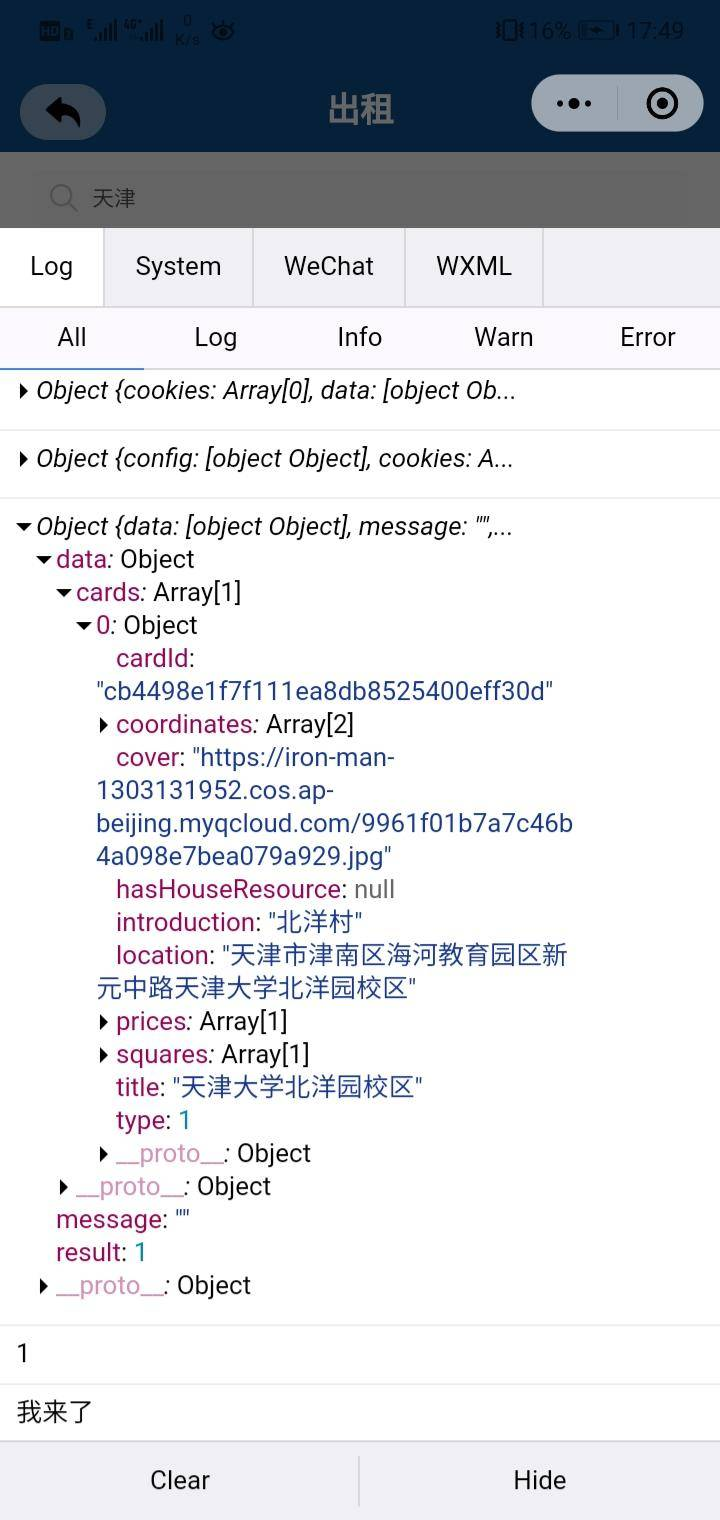
\includegraphics[width=3.8cm,height=8cm]{test/image/test24.png}
    \caption{测试结果}
    \end{minipage}
    \end{figure}
   
\section{帖子详情功能测试}
实现用例1:房屋信息查询

功能描述:用户可以查看帖子的详细信息

用户操作:点击帖子列表中的帖子,可进入对应帖子的详情页

预期结果:页面跳转到”首页“

测试结果:通过
\begin{figure}[htbp]
    \centering
    \begin{minipage}[t]{0.48\textwidth}
        \centering
        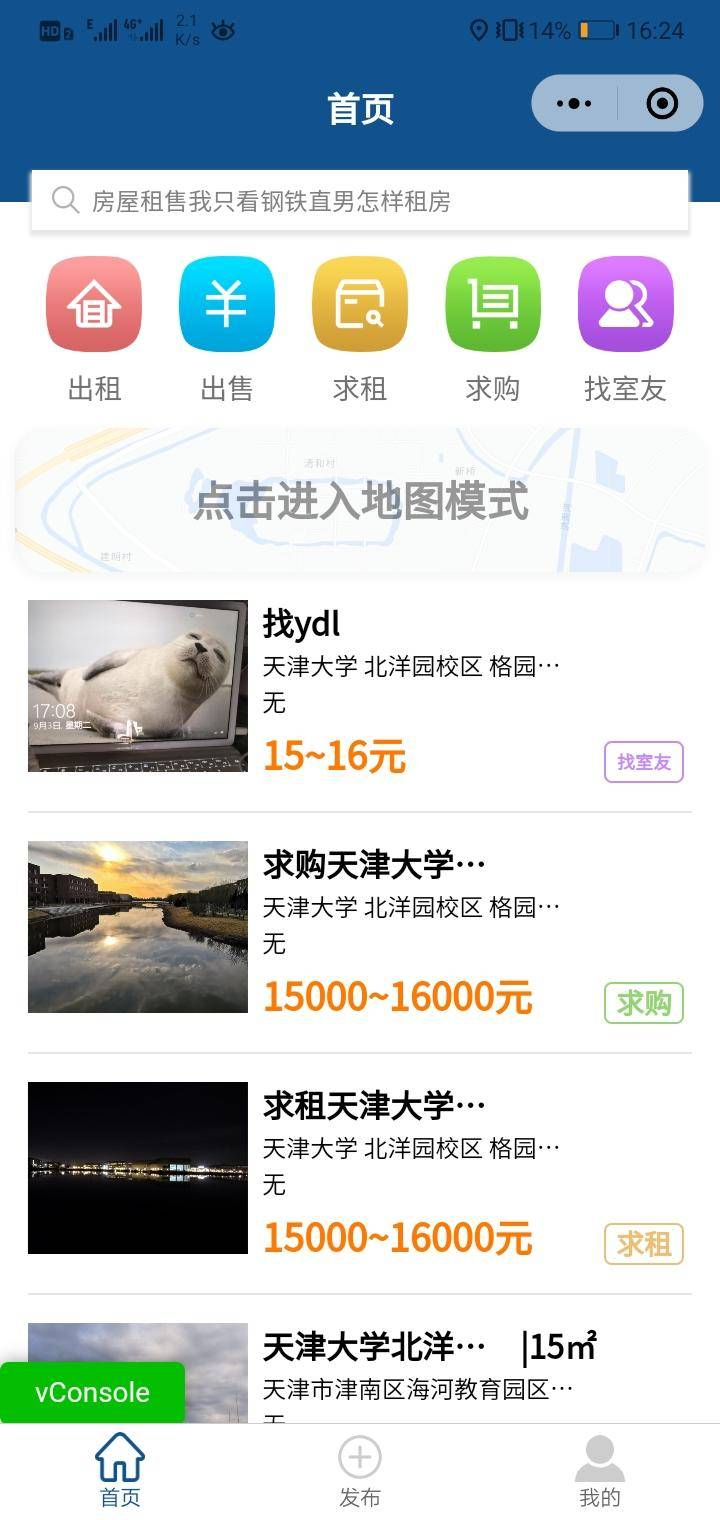
\includegraphics[width=4cm,height=8cm]{test/image/test16.png} 
       \caption{查看帖子详情} 
        \end{minipage}
   
    \end{figure}
   \newpage 
\section{发布出租帖子功能测试}

实现用例9:发布房屋出租信息

功能描述:用户可以填写房屋信息和要求,发布房屋出租信息

用户操作:在”发布“界面点击”我要出租“按钮,进入信息填写界面,填写后点击发布

预期结果:页面跳转到”首页“

测试结果:通过
    \begin{figure}[htbp]
        \centering
        \begin{minipage}[t]{0.48\textwidth}
        \centering
        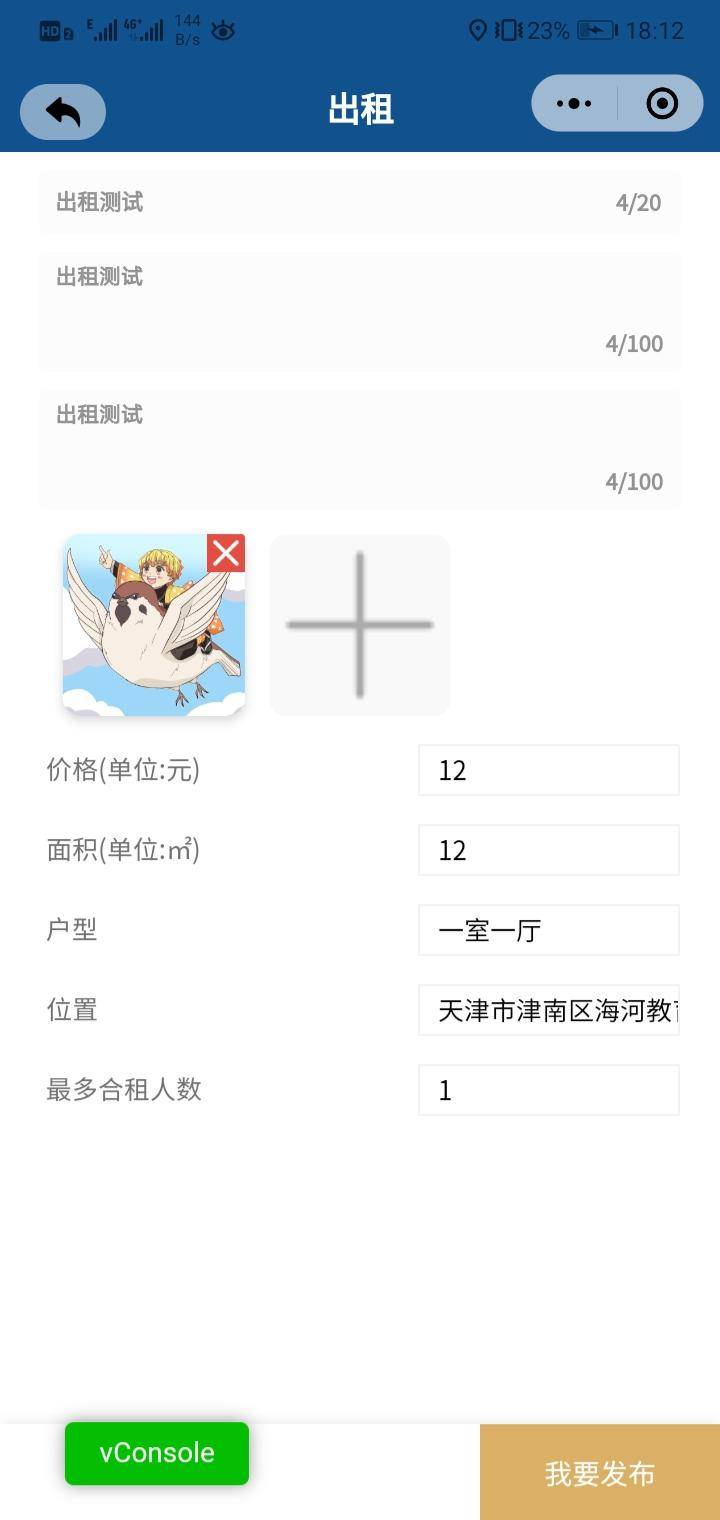
\includegraphics[width=4cm,height=8cm]{test/image/test26.png} 
     
       \caption{发布出租信息} 
        \end{minipage}
        \begin{minipage}[t]{0.48\textwidth}
        \centering
        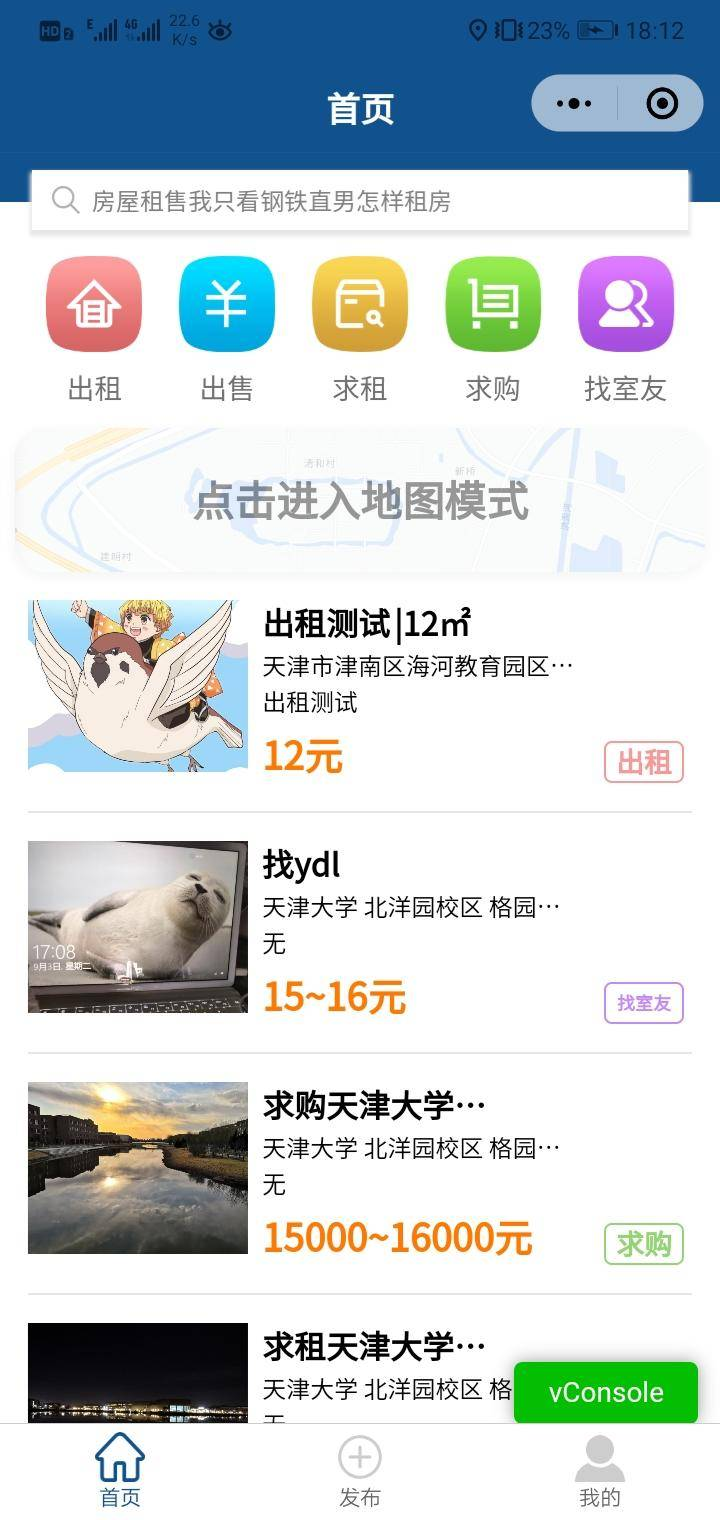
\includegraphics[width=4cm,height=8cm]{test/image/test27.png}
        \caption{测试结果}
        \end{minipage}
        \end{figure}
 
\section{发布出售帖子功能测试}

实现用例5:发布房屋出售信息

功能描述:用户可以填写房屋信息和要求,发布房屋出售信息

用户操作:在”发布“界面点击”我要出售“按钮,进入信息填写界面,填写后点击发布

预期结果:页面跳转到”首页“

测试结果:通过
\newpage 
    \begin{figure}[htbp]
        \centering
        \begin{minipage}[t]{0.48\textwidth}
        \centering
        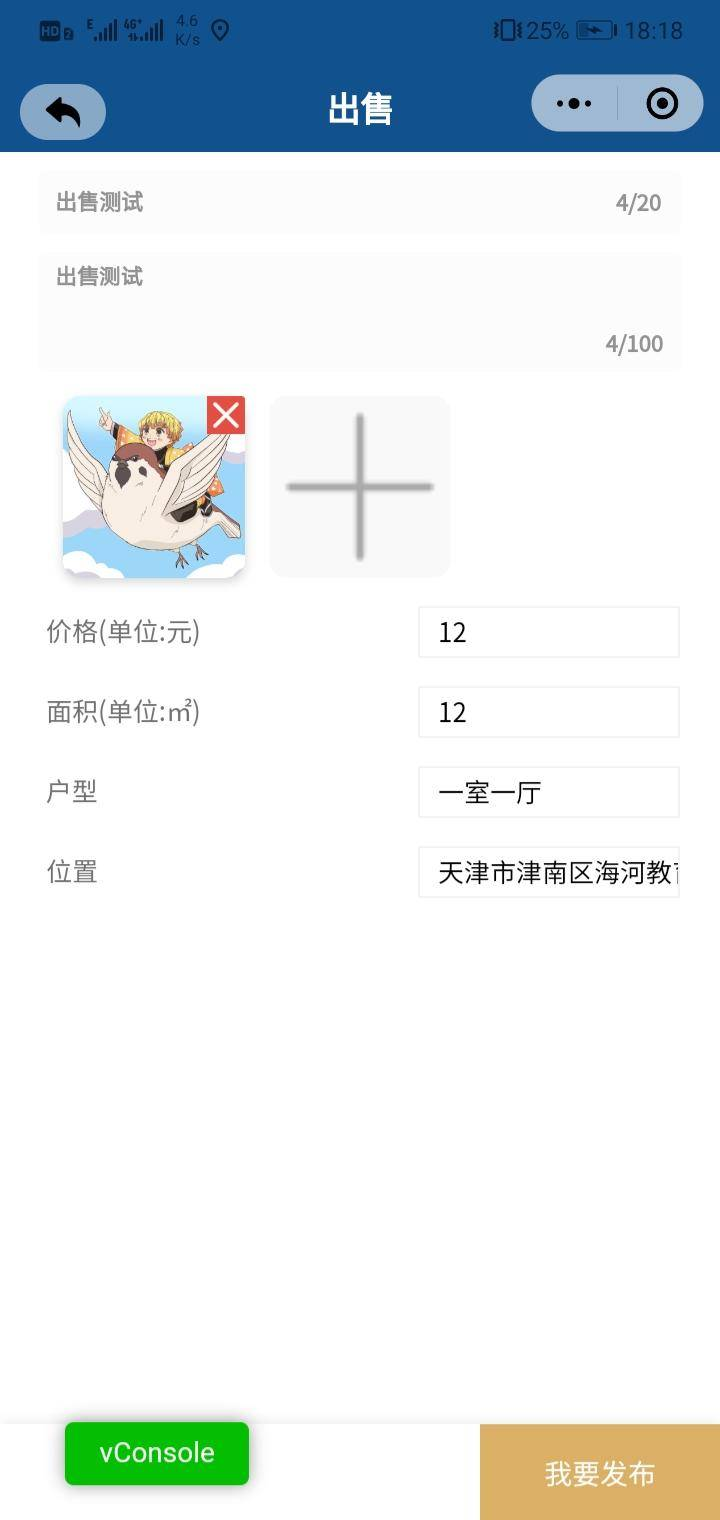
\includegraphics[width=4cm,height=8cm]{test/image/test28.png} 
     
       \caption{发布出售信息} 
        \end{minipage}
        \begin{minipage}[t]{0.48\textwidth}
        \centering
        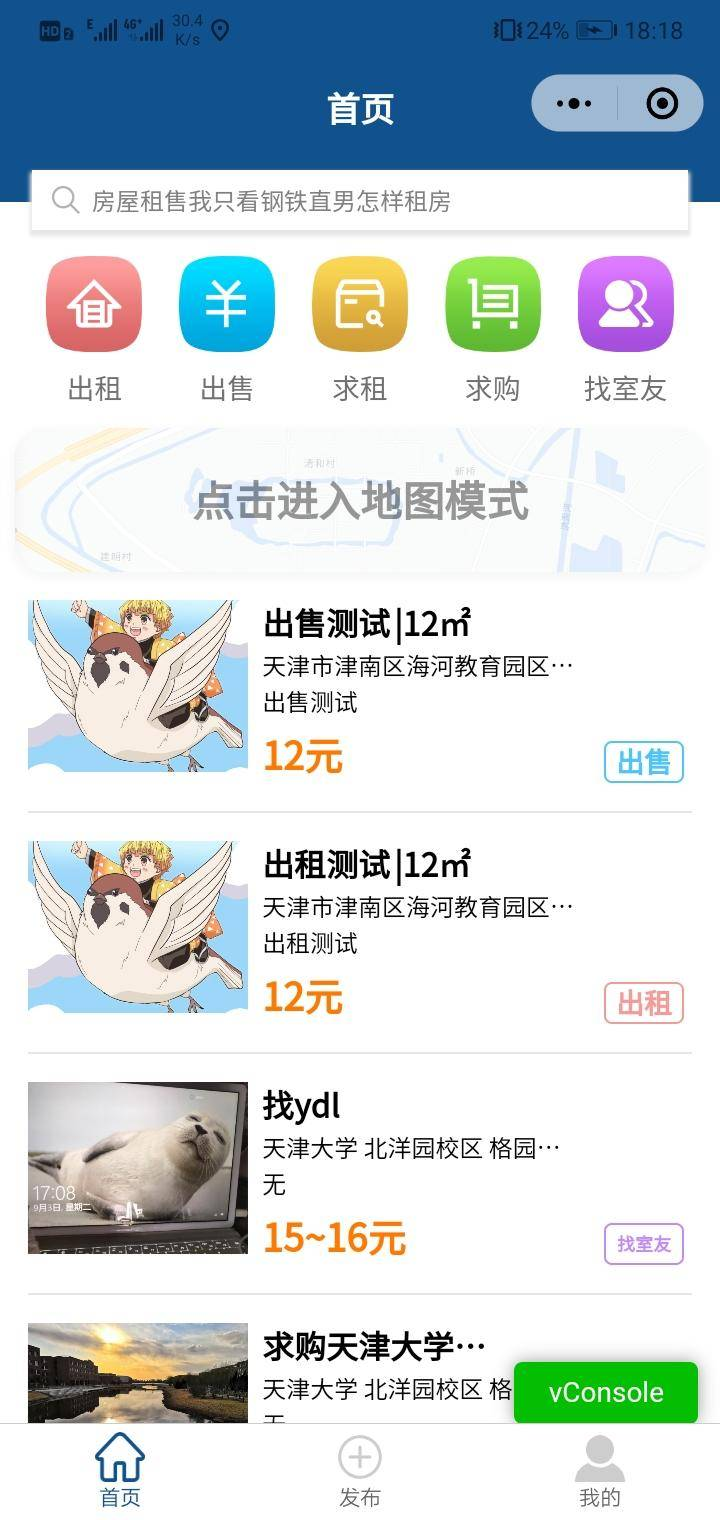
\includegraphics[width=4cm,height=8cm]{test/image/test29.png}
        \caption{测试结果}
        \end{minipage}
        \end{figure}

   \section{发布求租房帖子功能测试}

实现用例12:房屋信息查询

功能描述:用户可以填写对房屋的期望,发布房屋求租信息

用户操作:在”发布“界面点击”我要求租“按钮,进入信息填写界面,填写后点击发布

预期结果:页面跳转到”首页“

测试结果:通过
\begin{figure}[htbp]
    \centering
    \begin{minipage}[t]{0.48\textwidth}
    \centering
    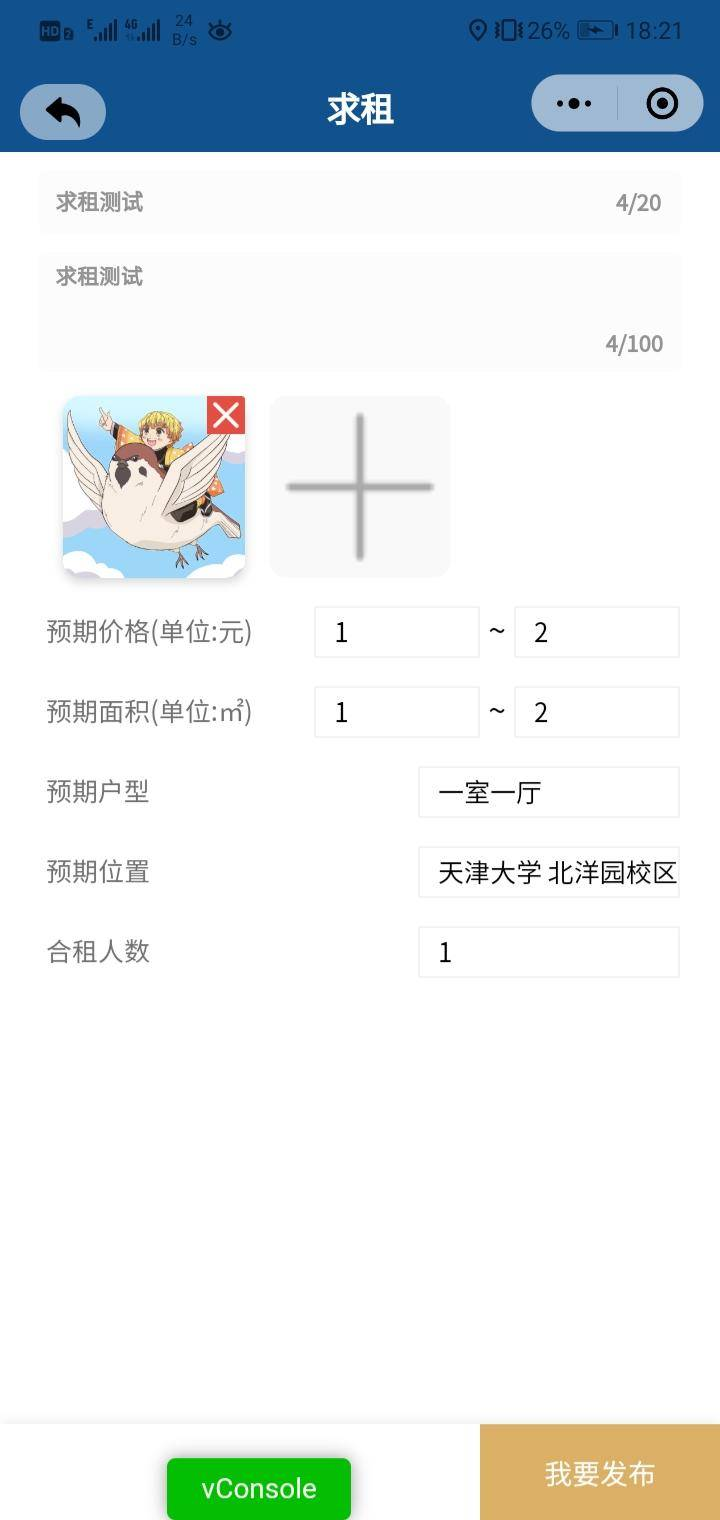
\includegraphics[width=4cm,height=8cm]{test/image/test30.png} 
 
   \caption{发布出售信息} 
    \end{minipage}
    \begin{minipage}[t]{0.48\textwidth}
    \centering
    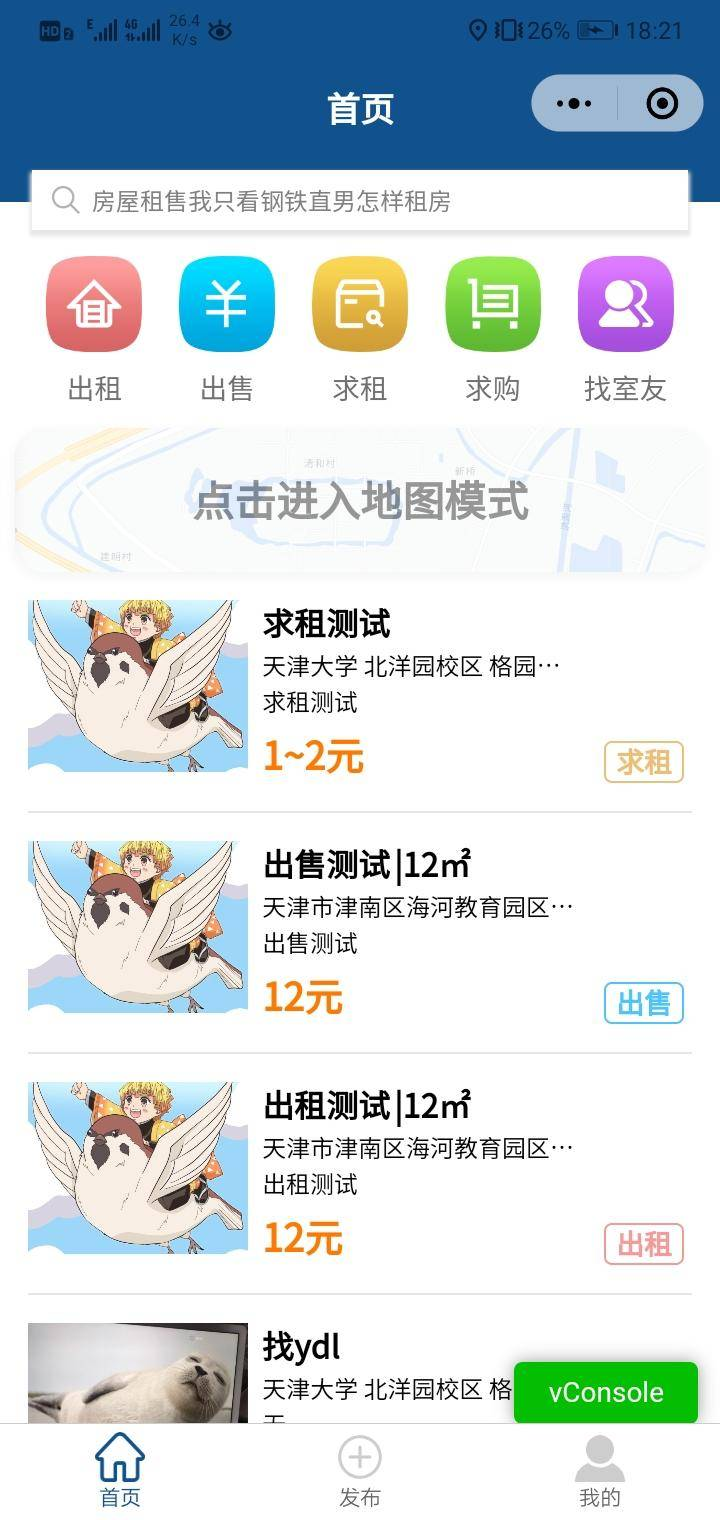
\includegraphics[width=4cm,height=8cm]{test/image/test31.png}
    \caption{测试结果}
    \end{minipage}
    \end{figure}
   \newpage 

   \section{发布求购帖子功能测试}

实现用例14:发出求购信息

功能描述:用户可以填写对房屋的期望,发布房屋求购信息

用户操作:在”发布“界面点击”我要求购“按钮,进入信息填写界面,填写后点击发布

预期结果:页面跳转到”首页“

测试结果:通过
\begin{figure}[htbp]
    \centering
    \begin{minipage}[t]{0.48\textwidth}
    \centering
    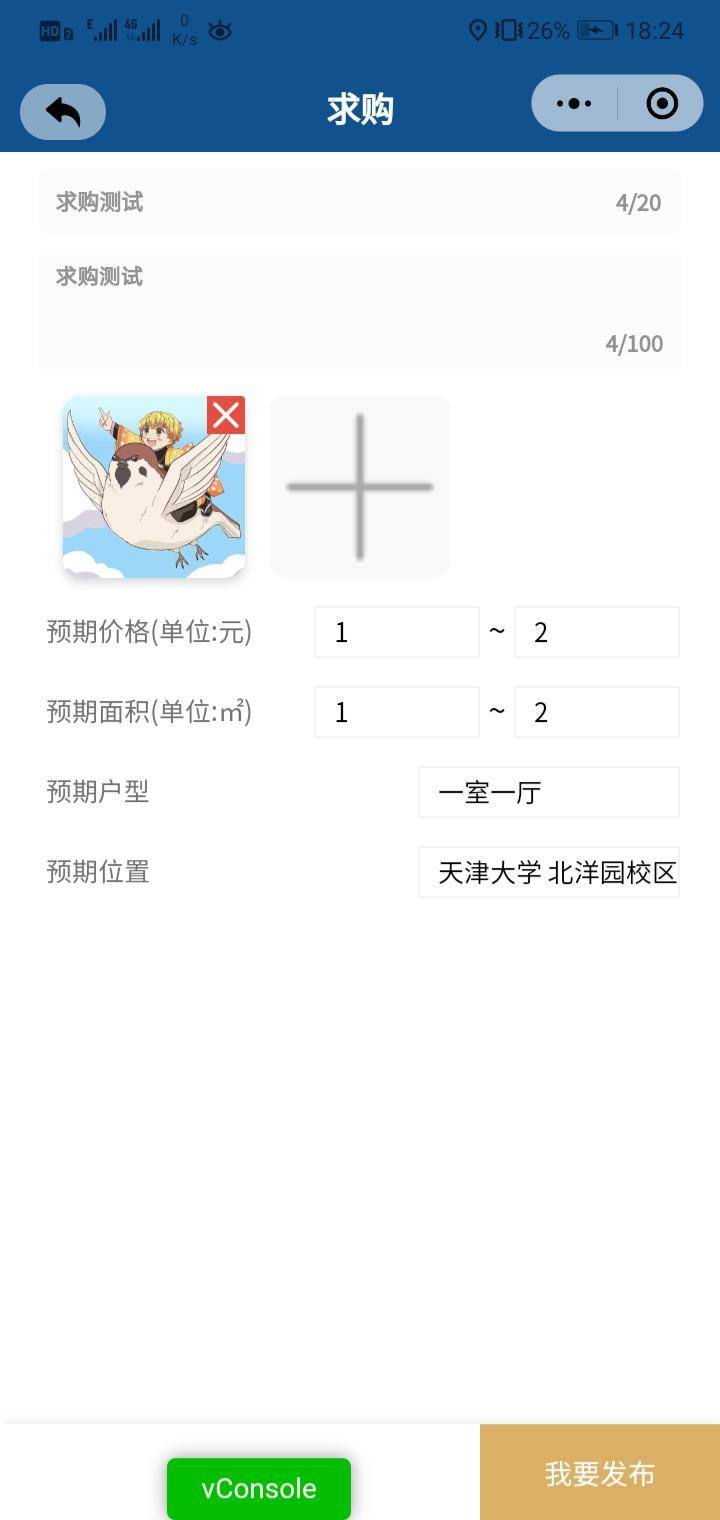
\includegraphics[width=4cm,height=8cm]{test/image/test32.png} 
 
   \caption{发布求购信息} 
    \end{minipage}
    \begin{minipage}[t]{0.48\textwidth}
    \centering
    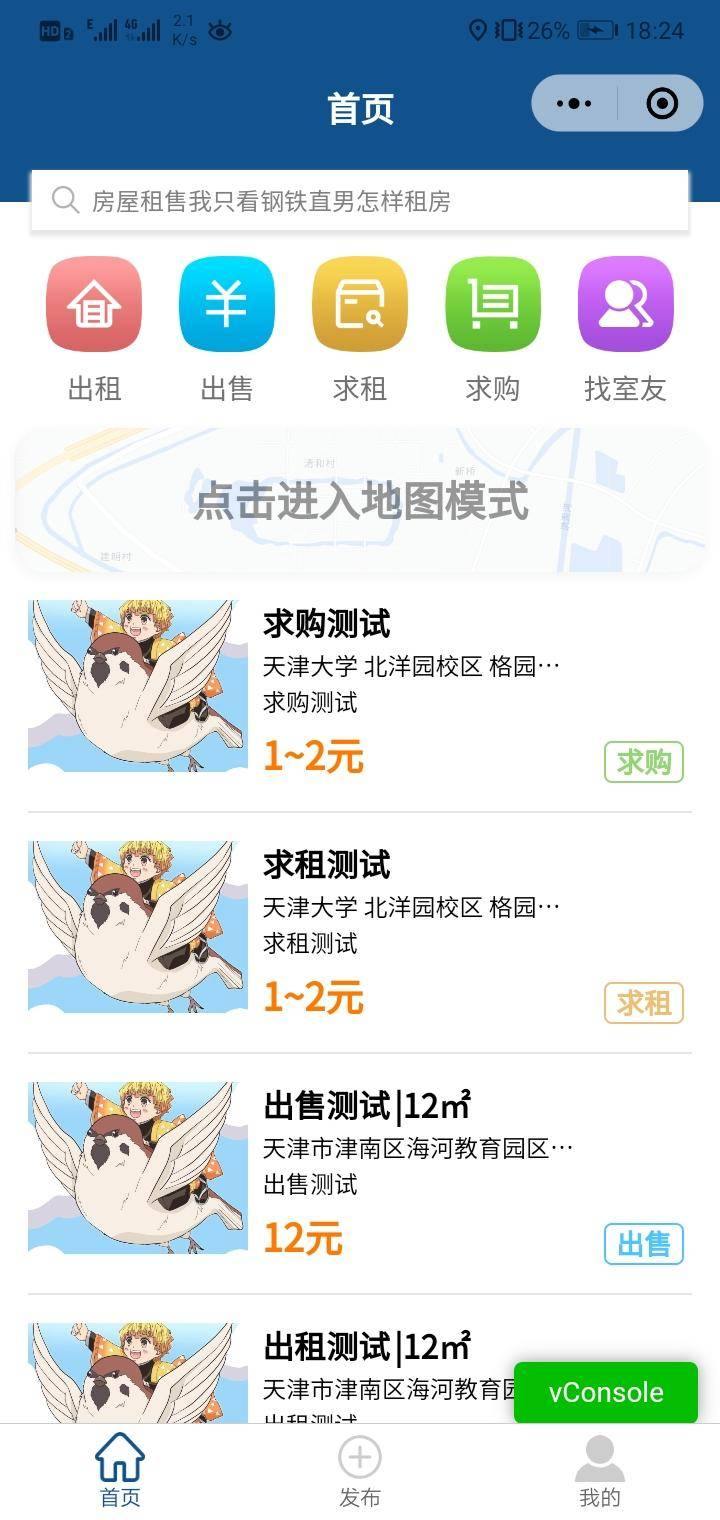
\includegraphics[width=4cm,height=8cm]{test/image/test33.png}
    \caption{测试结果}
    \end{minipage}
    \end{figure} 

   \section{发布找室友帖子功能测试}

实现用例10:发布找室友信息

功能描述:用户可以发布找室友信息

用户操作:在”发布“界面点击”我要找室友“按钮,进入信息填写界面,填写后点击发布

预期结果:页面跳转到”首页“

测试结果:通过
\newpage 
\begin{figure}[htbp]
    \centering
    \begin{minipage}[t]{0.48\textwidth}
    \centering
    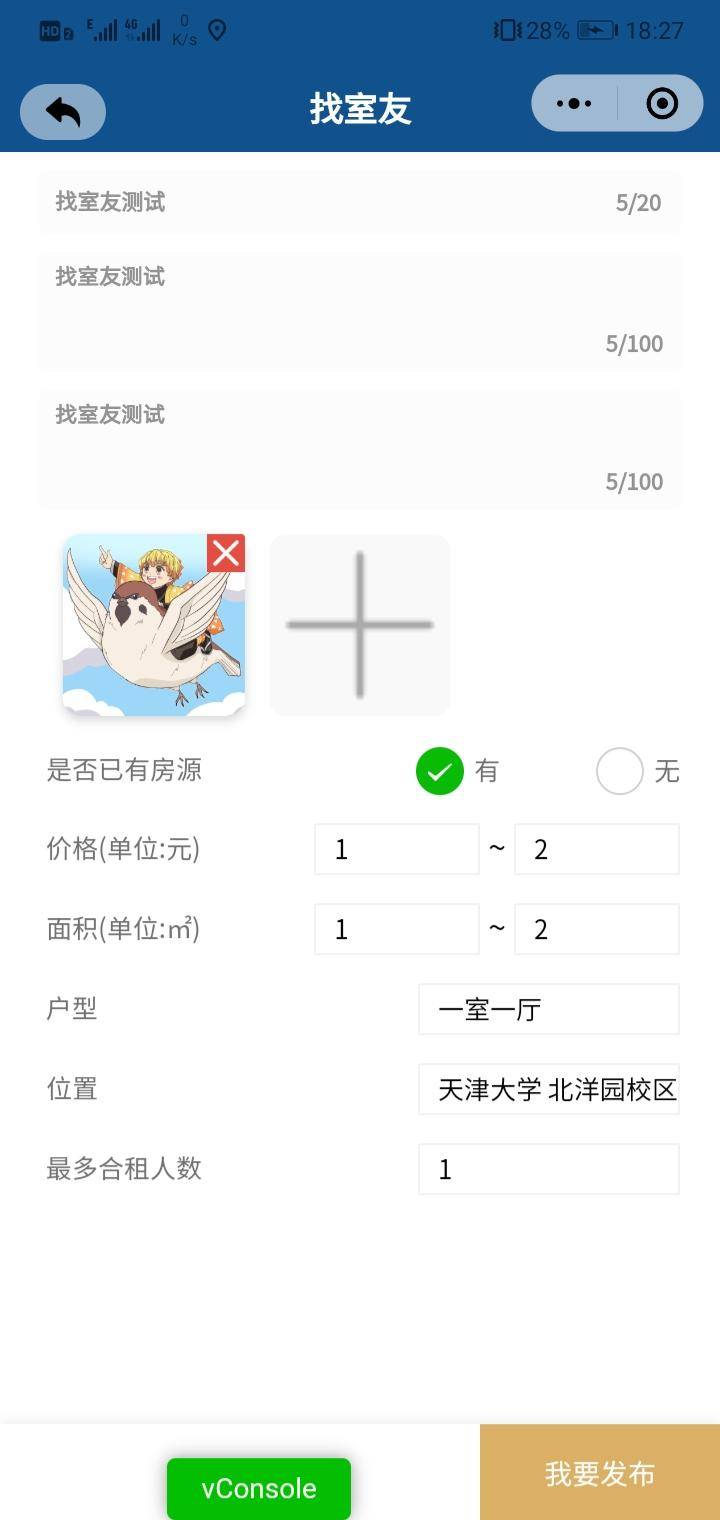
\includegraphics[width=4cm,height=8cm]{test/image/test34.png} 
 
   \caption{发布找室友信息} 
    \end{minipage}
    \begin{minipage}[t]{0.48\textwidth}
    \centering
    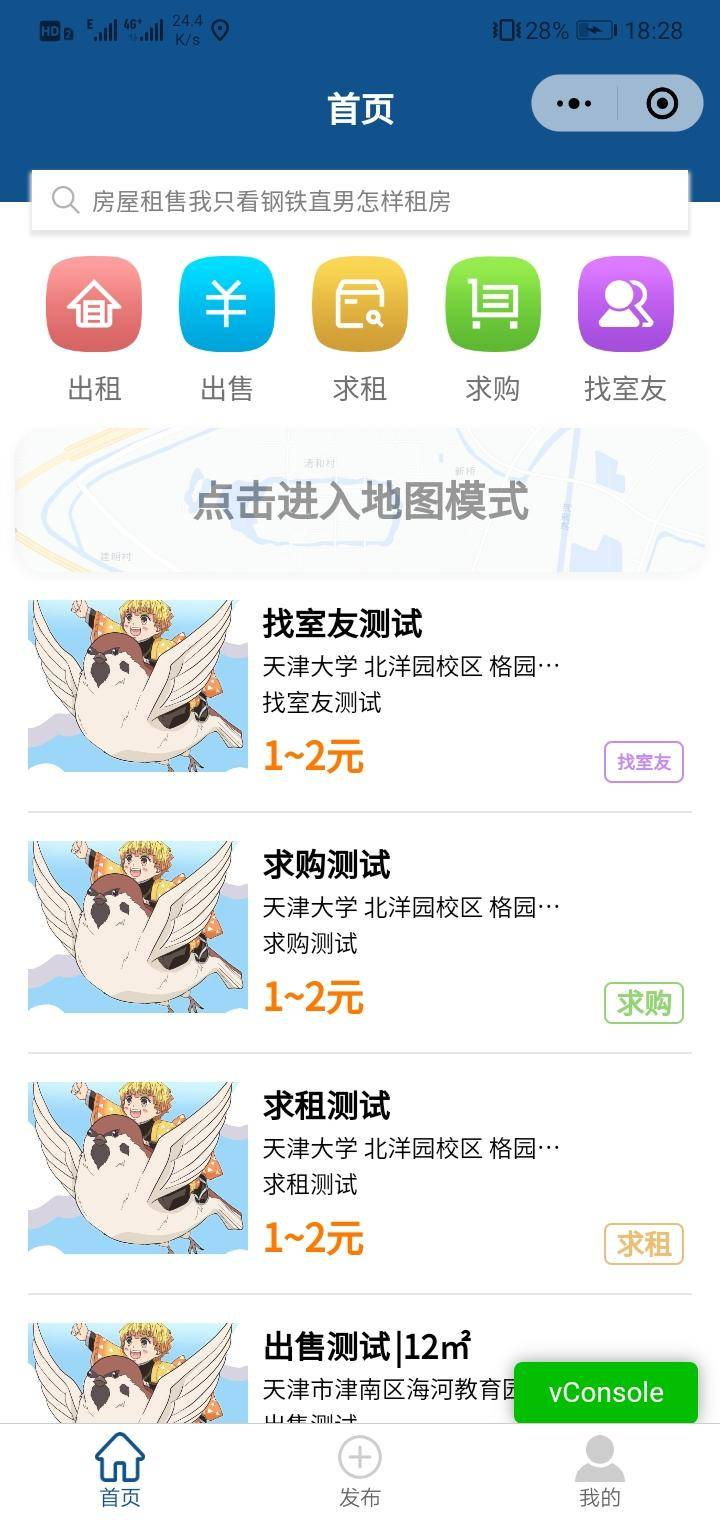
\includegraphics[width=4cm,height=8cm]{test/image/test35.png}
    \caption{测试结果}
    \end{minipage}
    \end{figure}


   \section{管理帖子功能测试}

   实现用例6,8,11,13,15:管理出售房屋信息,管理出租房屋信息,管理找室友信息,管理求租信息,管理求购信息

   功能描述:用户可以管理自己发布的出售、出租、找室友、求租、求购帖子
   
   用户操作:用户点击自己发出的帖子,进入详情页后可以删除该帖子
   
   预期结果:页面跳转到”首页“
   
   测试结果:通过
   
   \begin{figure}[htbp]
       \centering
       \begin{minipage}[t]{0.48\textwidth}
       \centering
       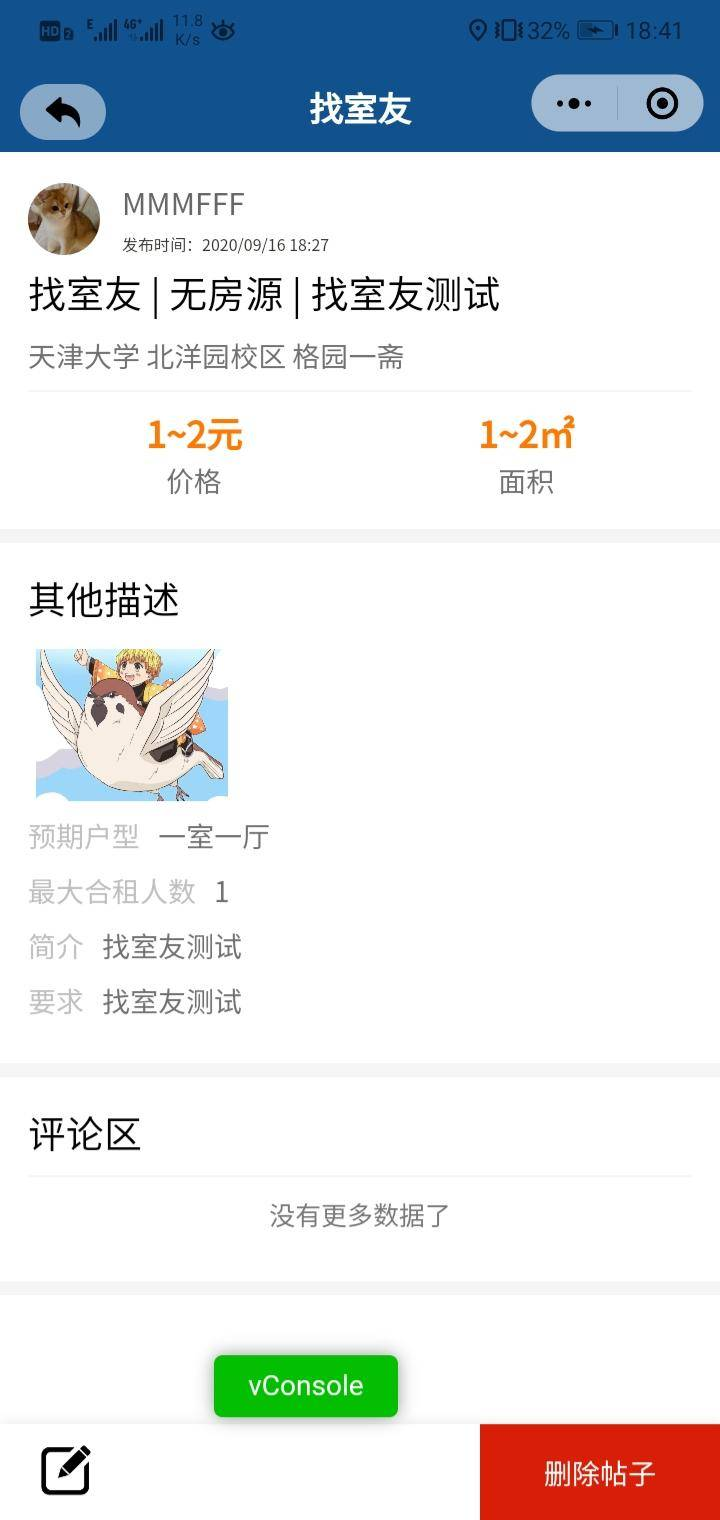
\includegraphics[width=4cm,height=8cm]{test/image/test36.png} 
    
      \caption{管理帖子} 
       \end{minipage}
       \begin{minipage}[t]{0.48\textwidth}
       \centering
       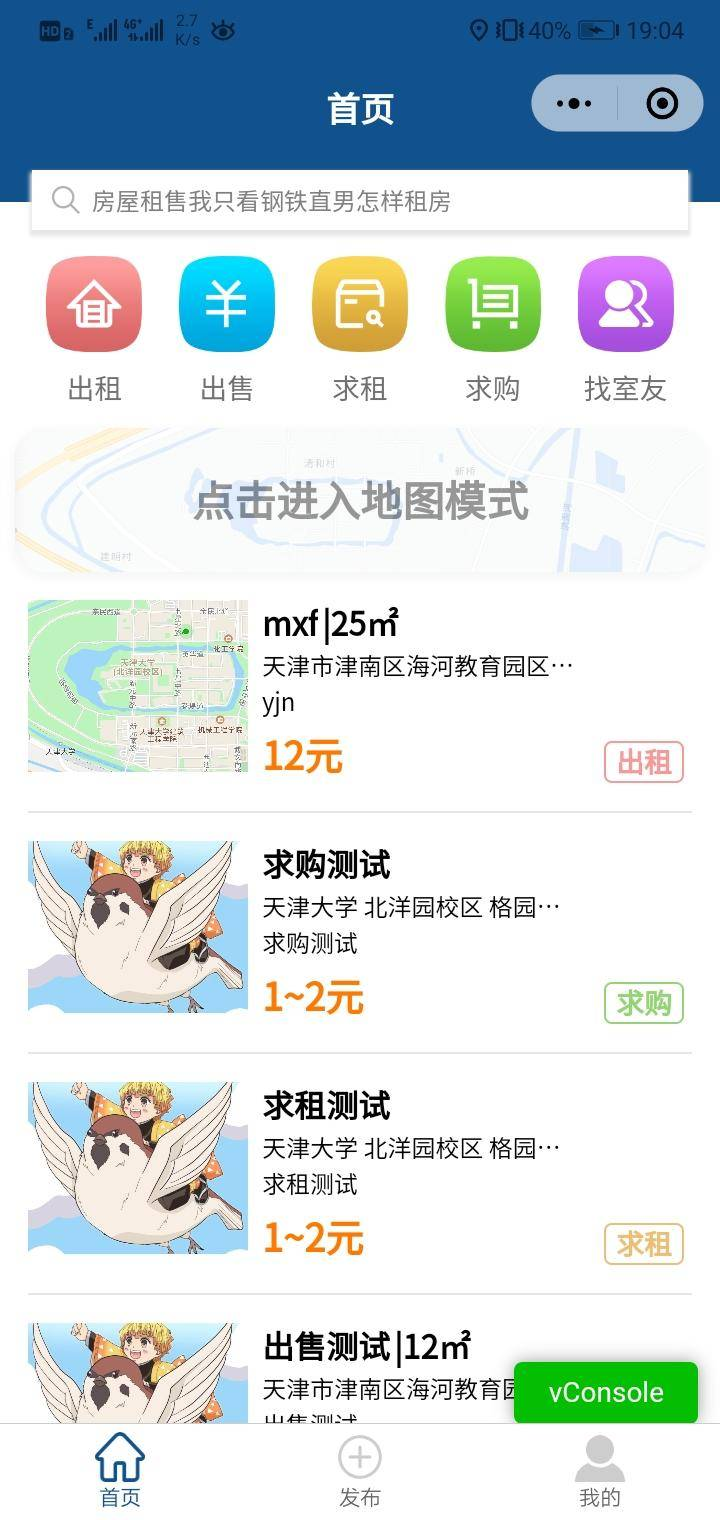
\includegraphics[width=4cm,height=8cm]{test/image/test37.png}
       \caption{结果}
       \end{minipage}
       \end{figure}
      \newpage 

   \section{评论功能测试}

   实现用例2:评论留言功能

   功能描述:用户可以在他人的帖子下发表评论,也可回复他人评论
   
   用户操作:用户点击详情页中的写评论图标,填写评论点击确定
   
   预期结果:帖子下方出现发表的评论
   
   测试结果:通过
   
   \begin{figure}[htbp]
       \centering
       \begin{minipage}[t]{0.48\textwidth}
       \centering
       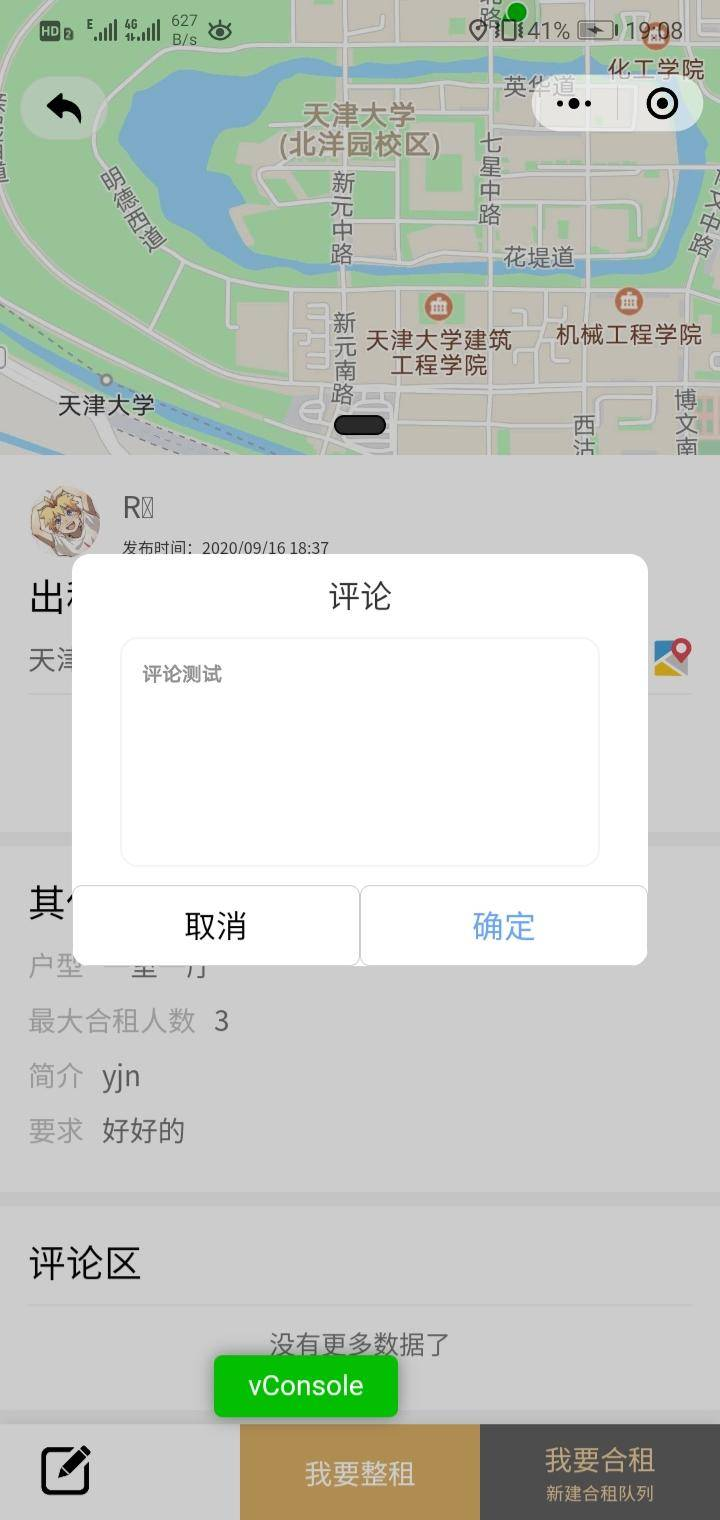
\includegraphics[width=4cm,height=8cm]{test/image/test38.png} 
    
      \caption{评论} 
       \end{minipage}
       \begin{minipage}[t]{0.48\textwidth}
        \centering
        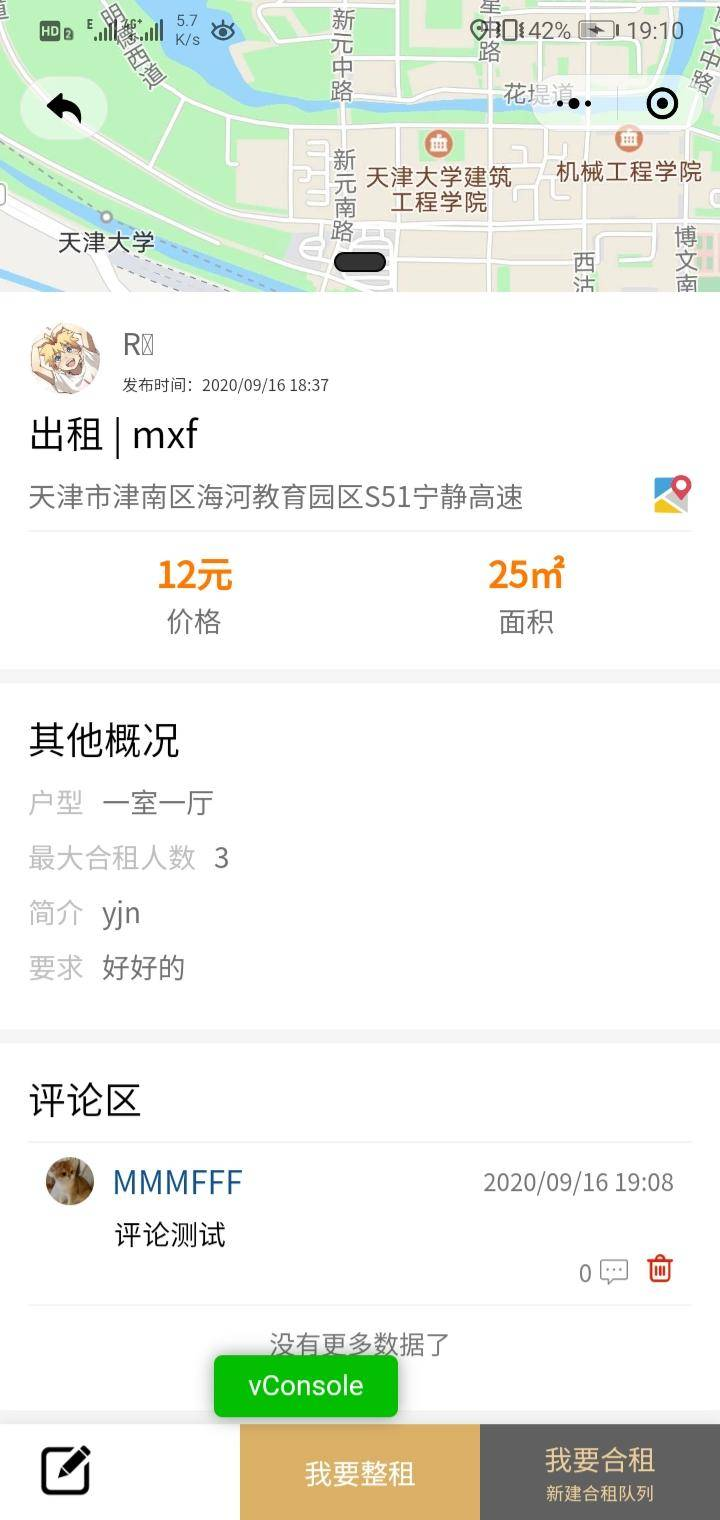
\includegraphics[width=4cm,height=8cm]{test/image/test39.png} 
     
       \caption{结果} 
         \end{minipage}
       \end{figure}
 
   \section{创建合租队列功能测试}
 
   功能描述:用户可以在他人的出租帖子下创建合租队列
   
   用户操作:用户点击详情页中的我要合租按钮 点击确定
   
   预期结果:帖子下方出现用户的合租队列
   
   测试结果:通过
   \newpage 
   \begin{figure}[htbp]
       \centering
       \begin{minipage}[t]{0.48\textwidth}
       \centering
       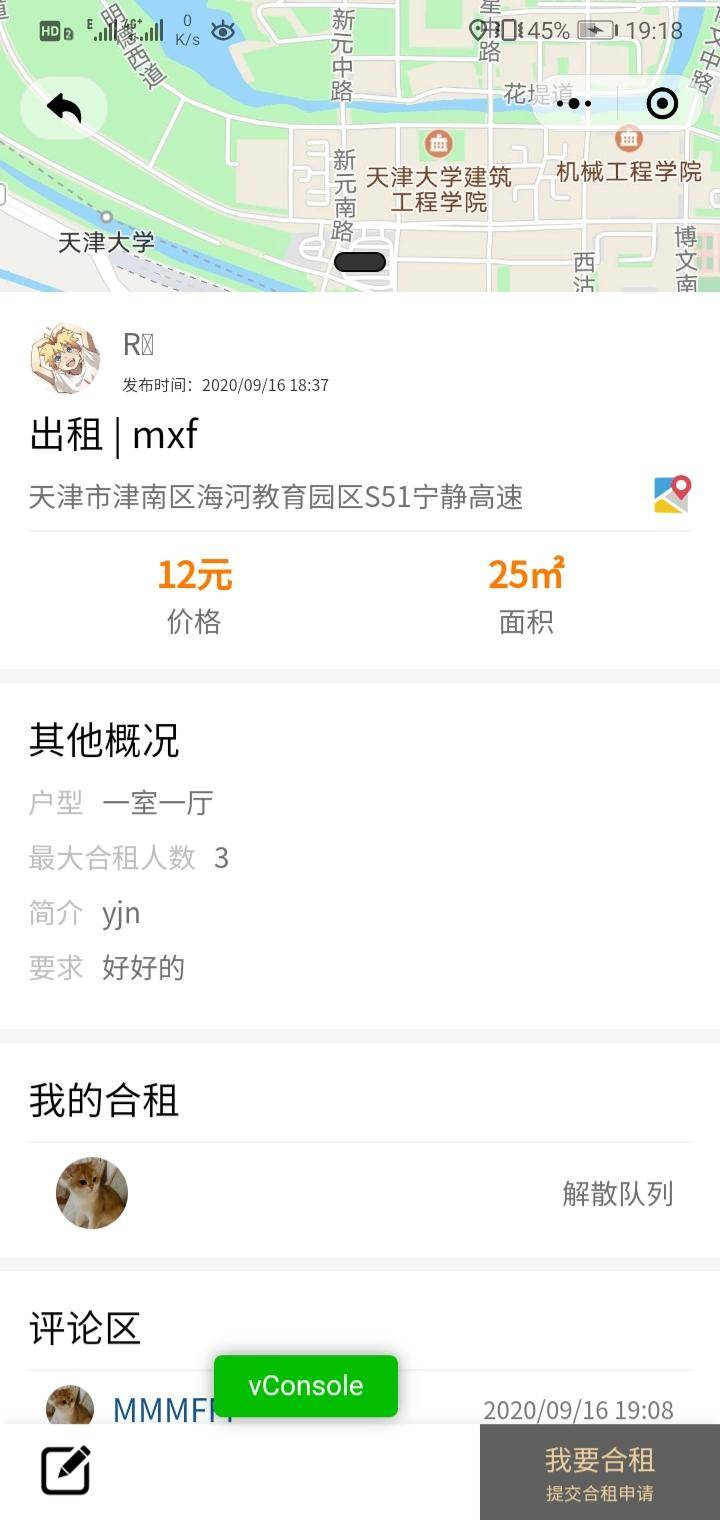
\includegraphics[width=4cm,height=8cm]{test/image/test40.png} 
    
      \caption{创建合租队列功能测试} 
       \end{minipage}
        
       \end{figure}
 

   \section{加入合租队列功能测试}
   功能描述:用户可以加入他人的合租队列
   
   用户操作:用户点击详情页中合租队列后的加入按钮
   
   预期结果:帖子详情页出现我的队列
   
   测试结果:通过
   
   \begin{figure}[htbp]
       \centering
       \begin{minipage}[t]{0.48\textwidth}
       \centering
       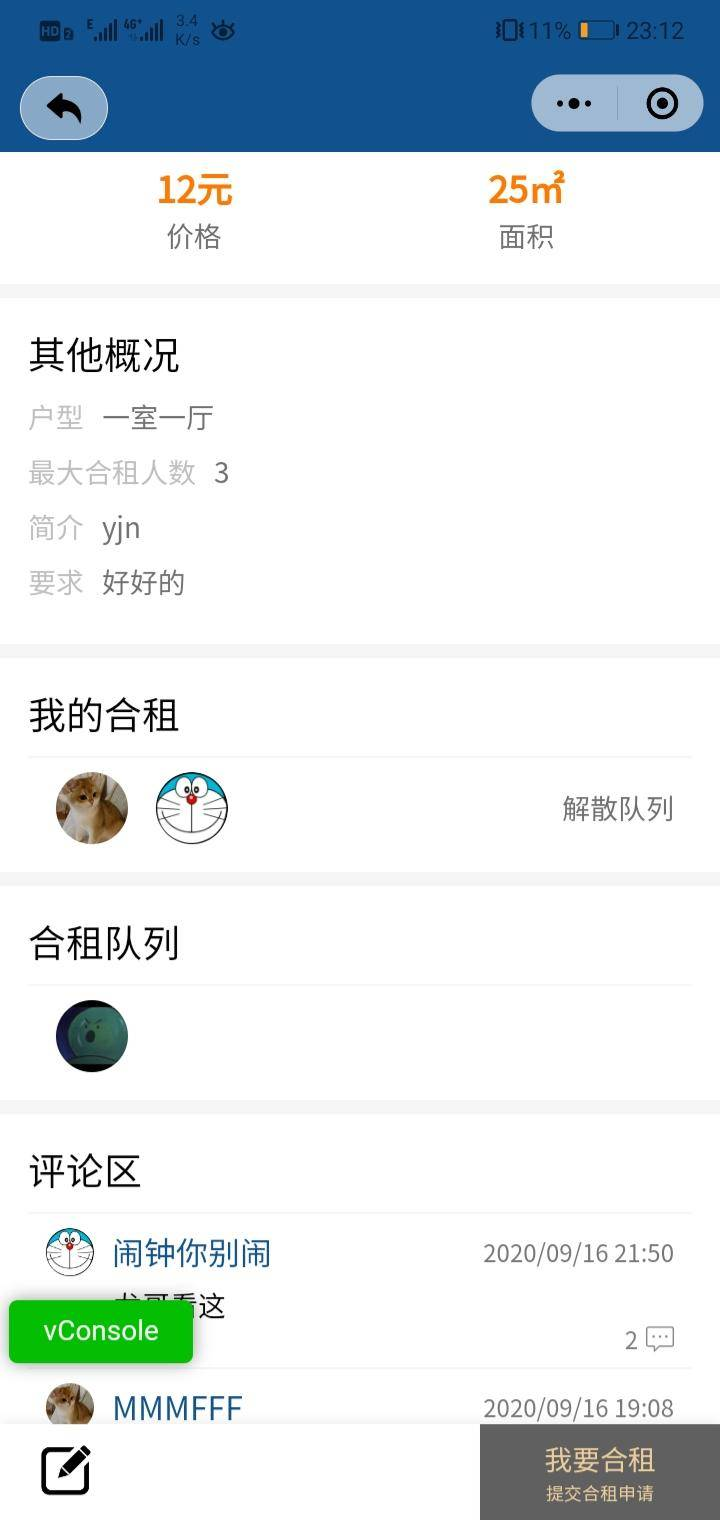
\includegraphics[width=4cm,height=8cm]{test/image/test41.png} 
    
      \caption{加入合租列队功能测试} 
    \end{minipage}
       \end{figure}
      \newpage 

   \section{删除合租队列功能测试}
 
   功能描述:合租队伍 发起者可以解散合租队伍
   
   用户操作:用户点击自己队伍旁的解散队伍按钮,并点击确定
   
   预期结果:详情页中自己的合租队伍被删除   
   
   测试结果:通过
   
   \begin{figure}[htbp]
       \centering
       \begin{minipage}[t]{0.48\textwidth}
       \centering
       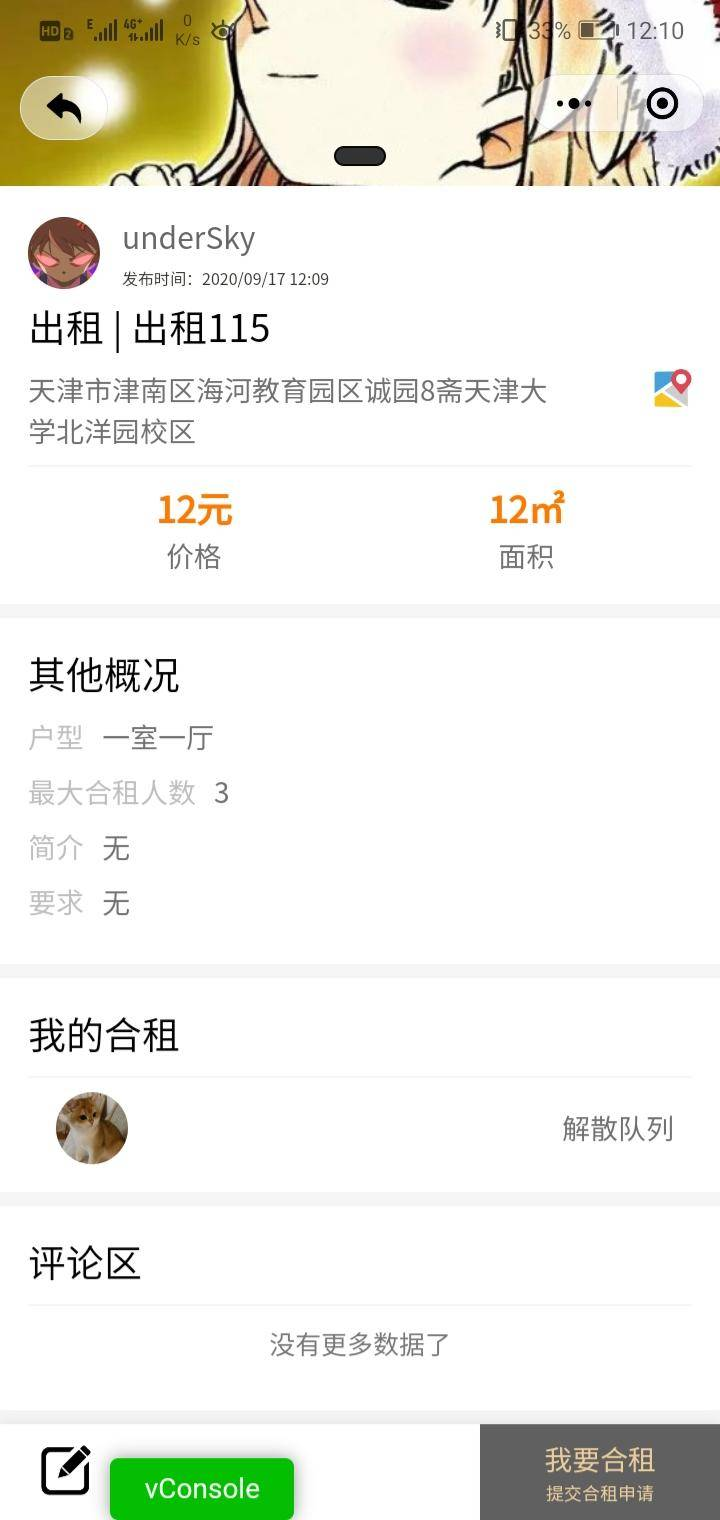
\includegraphics[width=4cm,height=8cm]{test/image/test42.png} 
    
      \caption{删除合租队列功能测试} 
       \end{minipage}
       \begin{minipage}[t]{0.48\textwidth}
       \centering
       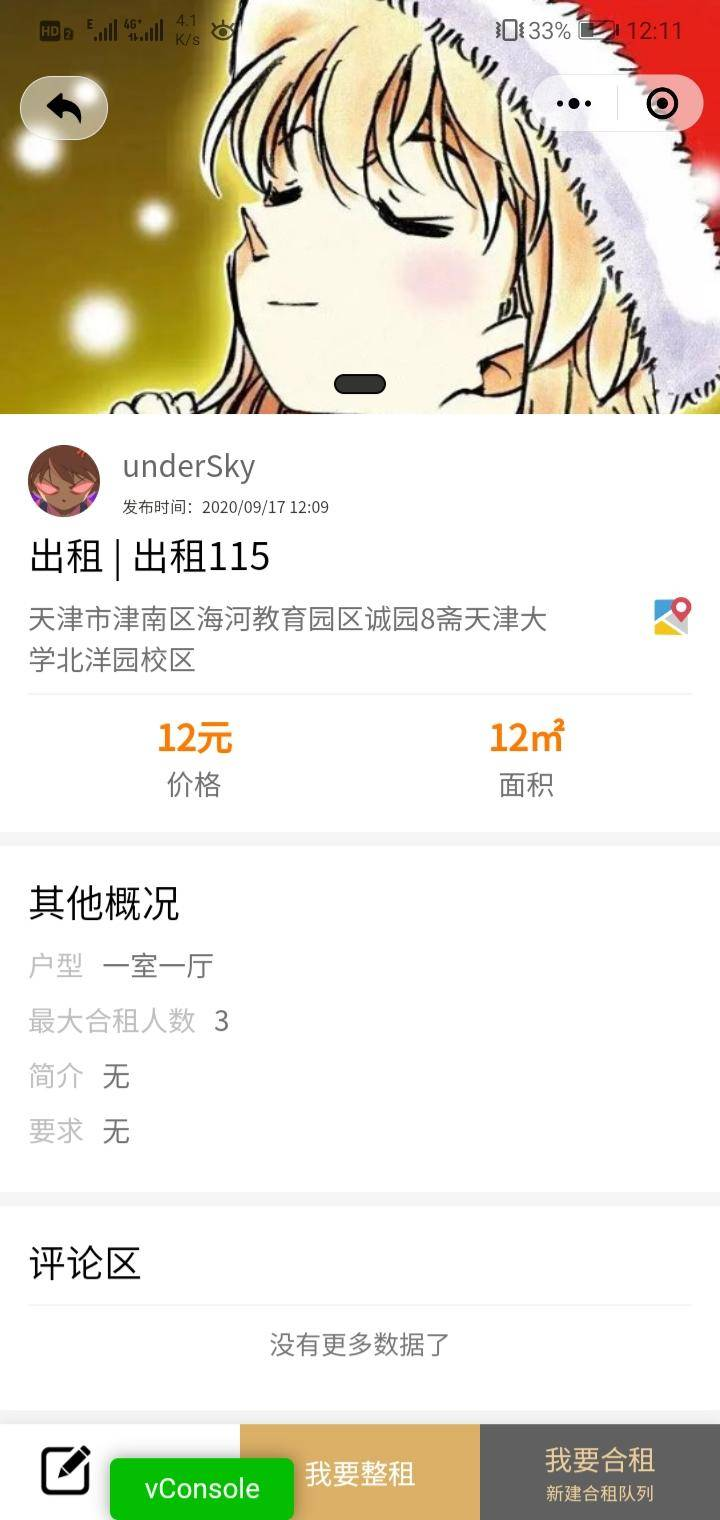
\includegraphics[width=4cm,height=8cm]{test/image/test43.png}
       \caption{测试结果}
       \end{minipage}
       \end{figure}
   
   \section{同意帖子功能测试}
   功能描述:1.用户可以以合租队长身份或个人身份向房住发出租房申请2.用户可以以个人身份向帖子主发出租房/购房/提供房源/找室友/的请求
   
   用户操作:用户以队长身份点击”发出申请“按钮或以个人身份点击我要“整租”
   
   预期结果:帖子主可以在帖子中看到他人的申请
   
   测试结果:通过
   \newpage 
   \begin{figure}[htbp]
       \centering
       \begin{minipage}[t]{0.48\textwidth}
       \centering
       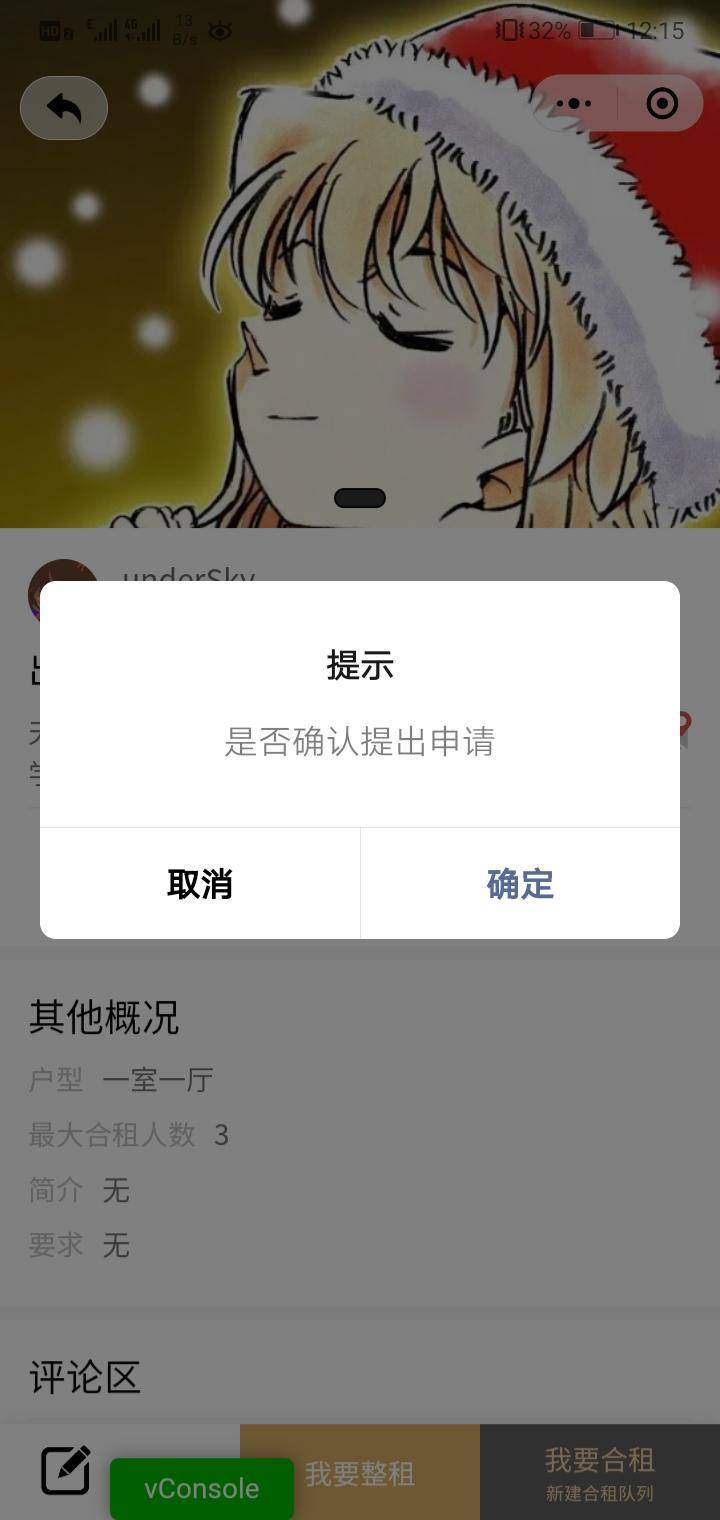
\includegraphics[width=4cm,height=8cm]{test/image/test44.png} 
    
      \caption{合租申请} 
    \end{minipage}
      \begin{minipage}[t]{0.48\textwidth}
        \centering
        \includegraphics[width=4cm,height=8cm]{test/image/test45.png} 
     
       \caption{整租申请} 
        \end{minipage}
       \end{figure}
    
   \section{同意申请功能测试}
   完成用例4:接单

   功能描述:帖子主可以同意他人的申请
   
   用户操作:用户在帖子详情页可以点击申请队列处的同意申请
   
   预期结果:同意后帖子被转至已完成
   
   测试结果:通过
   
   \begin{figure}[htbp]
       \centering
       \begin{minipage}[t]{0.48\textwidth}
       \centering
       \includegraphics[width=4cm,height=8cm]{test/image/test46.png} 
    
      \caption{申请功能测试} 
             \end{minipage}
       \end{figure}
      \newpage 
   \section{查看未完成帖子功能测试}
 
   功能描述:用户可以查看自己发出请求和发布的未完成的帖子
   
   用户操作:用户在“我的”页面下点击”未完成订单“按钮
   
   预期结果:页面跳转到”未完成订单
   
   测试结果:通过
 
   \begin{figure}[htbp]
       \centering
       \begin{minipage}[t]{0.48\textwidth}
       \centering
       \includegraphics[width=4cm,height=8cm]{test/image/test47.png} 
    
      \caption{搜索结果} 
       \end{minipage}
       \begin{minipage}[t]{0.48\textwidth}
       \centering
       \includegraphics[width=4cm,height=8cm]{test/image/test48.png}
       \caption{未完成界面}
       \end{minipage}
       \end{figure}
    
   \section{查看已完成帖子功能测试}
   功能描述:用户可以查看自己发出请求和发布的已完成的帖子,
   
   用户操作:用户在“我的”页面下点击”已完成订单“按钮
   
   预期结果:页面跳转到”已完成订单“
   
   测试结果:通过
   
   \begin{figure}[htbp]
       \centering
       \begin{minipage}[t]{0.48\textwidth}
       \centering
       \includegraphics[width=4cm,height=8cm]{test/image/test49.png} 
    
      \caption{我的界面} 
       \end{minipage}
       \begin{minipage}[t]{0.48\textwidth}
        \centering
        \includegraphics[width=4cm,height=8cm]{test/image/test50.png} 
     
       \caption{已完成界面}
    \end{minipage}
       \end{figure}
      \newpage 
   \section{查看通知功能测试}
   功能描述:用户可以查看其他用户发出的与自己有关的操作的提醒
   
   用户操作:用户点击“我的”可查看消息队列
   
   预期结果:页面跳转到”我的”页面
   
   测试结果:通过

   \begin{figure}[htbp]
       \centering
       \begin{minipage}[t]{0.48\textwidth}
       \centering
       \includegraphics[width=4cm,height=8cm]{test/image/test51.png} 
    
      \caption{通知} 
       \end{minipage}
 
       \end{figure}
       \newpage 
   \section{查看个人资料功能测试}
   完成用例18:查看用户信息

   功能描述:用户可以查看自己的个人资料
   
   用户操作:用户点击“我的”中的头像可以查看自己的个人信息
   
   预期结果:页面跳转到”个人信息”页面
   
   测试结果:通过
   
   \begin{figure}[htbp]
       \centering
       \begin{minipage}[t]{0.48\textwidth}
       \centering
       \includegraphics[width=4cm,height=8cm]{test/image/test52.png}
       \caption{个人信息界面}
       \end{minipage}
       \end{figure}
      \newpage 
   \section{修改个人资料功能测试}
   完成用例18:查看用户信息

   功能描述:用户可以修改自己的个人资料
   
   用户操作:可在个人信息界面修改个人信息
   
   预期结果:个人信息发生改变
   
   测试结果:个人简介修改,测试通过
   
   \begin{figure}[htbp]
       \centering
       \begin{minipage}[t]{0.48\textwidth}
       \centering
       \includegraphics[width=4cm,height=8cm]{test/image/test53.png} 
      \caption{个人信息界面} 
       \end{minipage}
       \begin{minipage}[t]{0.48\textwidth}
        \centering
        \includegraphics[width=4cm,height=8cm]{test/image/test55.png} 
       \caption{修改后} 
        \end{minipage}
       \end{figure}
      \newpage 

      \section{地图查看出租/出售帖子信息展示功能测试}
      完成用例1:房屋信息查询
   
      功能描述:用户可以在地图上查看出租/出售资源位置
      
      用户操作:用户点击“首页”的“点击进入地图模式”按钮
      
      预期结果:跳转到地图界面,地图上展示房屋资源
      
      测试结果:通过
      
      \begin{figure}[htbp]
          \centering
          \begin{minipage}[t]{0.48\textwidth}
          \centering
          \includegraphics[width=4cm,height=8cm]{test/image/test56.png} 
         \caption{个人信息界面} 
          \end{minipage}
          \begin{minipage}[t]{0.48\textwidth}
           \centering
           \includegraphics[width=4cm,height=8cm]{test/image/test57.png} 
          \caption{修改后} 
           \end{minipage}
          \end{figure}
         \newpage 
         \section{通过地图查看出租/出售帖子位置功能测试}
         完成用例1:房屋信息查询
      
         功能描述:用户可以在地图上查看指定出租/出售资源位置
         
         用户操作:用户点击“详情页”的“地图”按钮
         
         预期结果:跳转到地图界面,地图上展示房屋资源
         
         测试结果:通过
         
         \begin{figure}[htbp]
             \centering
             \begin{minipage}[t]{0.48\textwidth}
             \centering
             \includegraphics[width=4cm,height=8cm]{test/image/test58.png} 
            \caption{个人信息界面} 
             \end{minipage}
             \begin{minipage}[t]{0.48\textwidth}
              \centering
              \includegraphics[width=4cm,height=8cm]{test/image/test59.png} 
             \caption{修改后} 
              \end{minipage}
             \end{figure}
            \newpage                
	% !Mode:: "TeX:UTF-8"

\chapter{用例模型}

\section{确定用例}

\subsection{系统用例}

\begin{figure}[htbp]

    \centering
    
    \includegraphics[height=10.0cm,width=14.0cm]{requirement/figures/xitong.png} 
    \caption{系统用例图}
    
    \end{figure}
\newpage
\subsection{用户}
 
\begin{figure}[htbp]

    \centering
    
    \includegraphics[height=10.0cm,width=14.0cm]{requirement/figures/yonghu.png} 
    \caption{用户用例图}
    
    \end{figure}
    \newpage
\subsection{房主}

\begin{figure}[htbp]

    \centering
    
    \includegraphics[height=14.0cm,width=14.0cm]{requirement/figures/fangzhu.png} 
    \caption{房主用例图}
    
    \end{figure}
    \newpage

\subsection{租房者}

\begin{figure}[htbp]

    \centering
    
    \includegraphics[height=14.0cm,width=14.0cm]{requirement/figures/zufangzhe.png} 
    \caption{租房者用例图}
    
    \end{figure}
    \newpage
\subsection{购房者}

\begin{figure}[htbp]

    \centering
    
    \includegraphics[height=12.0cm,width=14.0cm]{requirement/figures/goufangzhe.png} 
    \caption{购房者用例图}
    
    \end{figure}
    \newpage
\subsection{管理员}
 
\begin{figure}[htbp]

    \centering
    
    \includegraphics[height=14.0cm,width=14.0cm]{requirement/figures/guanliyuan.png} 
    \caption{管理员用例图}
    
    \end{figure}
    \newpage

\section{描述用例规约}

% \begin{table}[htbp]
% 	\centering
% 	\begin{tabular}{|c|l|c|l|}
%         \hline
%         编号 & 1 & 名称 & 房屋信息查询 \\ 
%         \hline
%         执行者 & \multicolumn{3}{|p{11cm}|}{用户} \\
%         \hline
%         描述 & \multicolumn{3}{|p{11cm}|}{
%             用户查询房屋信息,能够找到心仪的出租、出售、求租、求售、找室友帖子
%         } \\
%         \hline
%         前置条件 & \multicolumn{3}{|p{11cm}|}{无} \\
%         \hline
%         基本流程 & \multicolumn{3}{|p{11cm}|}{       
%             \begin{itemize}
%                 \item 1.选择房屋筛选条件
%                 \item 2.展示符合条件的房屋
%                 \item 3.点击可进入房屋详情页面进行申请
%             \end{itemize} \\
%         } \\
%         \hline
%         结束状况 & \multicolumn{3}{|p{11cm}|}{系统展示符合条件的房屋信息} \\
%         \hline
%         可选流程 & \multicolumn{3}{|p{11cm}|}{无} \\
%         \hline
%         异常流程 & \multicolumn{3}{|p{11cm}|}{无} \\
%         \hline
%         说明 & \multicolumn{3}{|p{11cm}|}{无} \\
%         \hline
%     \end{tabular}
%     \caption{房屋信息查询}
% \end{table}

\begin{table}[htbp]
	\centering
	\begin{tabular}{|c|p{11cm}|}
        \hline
        编号 & 1 \\
        \hline
        名称 & 房屋信息查询 \\ 
        \hline
        执行者 &用户 \\
        \hline
        描述 & 用户查询房屋信息,能够找到心仪的出租、出售、求租、求售、找室友帖子        \\
        \hline
        前置条件 & 无 \\
        \hline
        基本流程 & \begin{itemize}
            \item 1.选择房屋筛选条件
            \item 2.展示符合条件的房屋
            \item  3.点击可进入房屋详情页面进行申请
        \end{itemize} \\
        \hline
        结束状况 &系统展示符合条件的房屋信息 \\
        \hline
        可选流程 & 无 \\
        \hline
        异常流程 & 无 \\
        \hline
        说明 & 无 \\
        \hline
    \end{tabular}
    \caption{房屋信息查询}
\end{table}

\begin{table}[htbp]
	\centering
	\begin{tabular}{|c|p{11cm}|}
        \hline
        编号 & 2.1 \\
        \hline
        名称 & 写评论 \\ 
        \hline
        执行者 &用户 \\
        \hline
        描述 & 每个页面(包括出租出售求租求购找室友)下方具有评论区, 供用户在此交流.        \\
        \hline
        前置条件 & 用户打开相关页面 \\
        \hline
        基本流程 & \begin{itemize}
            \item 1.编辑文本框
            \item 2.点击发送
        \end{itemize} \\
        \hline
        结束状况 & 消息发送成功 \\
        \hline
        可选流程 & 用户可以选择新建评论, 或者回复其它用户的评论 \\
        \hline
        异常流程 & 无 \\
        \hline
        说明 & 无 \\
        \hline
    \end{tabular}
    \caption{写评论}
\end{table}

\begin{table}[htbp]
	\centering
	\begin{tabular}{|c|p{11cm}|}
        \hline
        编号 & 2.2 \\ 
        \hline
        名称 & 收评论 \\ 
        \hline
        执行者 &用户 \\
        \hline
        描述 & 当其它用户发出与此用户相关的评论时, 在微信的消息列表中发送提示.        \\
        \hline
        前置条件 & 无 \\
        \hline
        基本流程 & \begin{itemize}
            \item 1. 微信消息列表中查看提示
            \item 2. 点击消息后跳转至相关页面
        \end{itemize} \\
        \hline
        结束状况 & 跳转至相关页面. \\
        \hline
        可选流程 & 无 \\
        \hline
        异常流程 & 无 \\
        \hline
        说明 & 无 \\
        \hline
    \end{tabular}
    \caption{收评论}
\end{table}

\begin{table}[htbp]
	\centering
	\begin{tabular}{|c|p{11cm}|}
        \hline
        编号 & 3.1 \\
        \hline
        名称 & 查看个人信息 \\ 
        \hline
        执行者 &用户 \\
        \hline
        描述 & 在个人主页中用户可以查看个人信息       \\
        \hline
        前置条件 & 无 \\
        \hline
        基本流程 & \begin{itemize}
            \item 1.点击个人信息按钮
            \item 2.展示个人信息
        \end{itemize} \\
        \hline
        结束状况 & 展示个人信息页面 \\
        \hline
        可选流程 & 无 \\
        \hline
        异常流程 & 无 \\
        \hline
        说明 & 无 \\
        \hline
    \end{tabular}
    \caption{查看个人信息}
\end{table}

\begin{table}[htbp]
	\centering
	\begin{tabular}{|c|p{11cm}|}
        \hline
        编号 & 3.2 \\
        \hline
        名称 & 房屋信息查询修改个人信息 \\ 
        \hline
        执行者 &用户 \\
        \hline
        描述 & 可以在个人主页中编辑自身相关信息        \\
        \hline
        前置条件 & 用户已经登陆 \\
        \hline
        基本流程 & \begin{itemize}
            \item 1. 点击按钮
            \item 2. 编辑相关文本框
            \item  3. 提交
        \end{itemize} \\
        \hline
        结束状况 & 点击提交, 提示成功 \\
        \hline
        可选流程 & 无 \\
        \hline
        异常流程 & 无 \\
        \hline
        说明 & 无 \\
        \hline
    \end{tabular}
    \caption{修改个人信息}
\end{table}

\begin{table}[htbp]
	\centering
	\begin{tabular}{|c|p{11cm}|}
        \hline
        编号 & 4 \\
        \hline
        名称 & 接单 \\ 
        \hline
        执行者 &用户 \\
        \hline
        描述 & 用户可以对于其他用户发布的出租/出售/求购/求租/找室友的帖子进行接单 \\
        \hline
        前置条件 & 已有出租/出售/求购/求租/找室友的帖子 \\
        \hline
        基本流程 & \begin{itemize}
            \item 1.点击提示框
            \item 2.进入相应事务页面
            \item 3.发出接单申请
        \end{itemize} \\
        \hline
        结束状况 & 接单成功 \\
        \hline
        可选流程 & \begin{itemize}
            \item 1.出租帖子建立拼单队列
            \item 2.拼单成功
            \item 3.发出接单申请
        \end{itemize} \\
        \hline
        异常流程 & 无 \\
        \hline
        说明 & 无 \\
        \hline
    \end{tabular}
    \caption{接单}
\end{table}

\begin{table}[htbp]
	\centering
	\begin{tabular}{|c|p{11cm}|}
        \hline
        编号 & 5 \\
        \hline
        名称 & 发布出售房屋信息 \\ 
        \hline
        执行者 & 房主 \\
        \hline
        描述 & 房主用户可以发布出售房屋的相关信息,  以提供给买房者参考.        \\
        \hline
        前置条件 & 无 \\
        \hline
        基本流程 & \begin{itemize}
            \item 1.进入相关页面
            \item 2.编辑房屋信息, 卖房信息, 定价和介绍等相关信息
            \item 3.点击发布
        \end{itemize} \\
        \hline
        结束状况 & 发布成功 \\
        \hline
        可选流程 & 无 \\
        \hline
        异常流程 & 无 \\
        \hline
        说明 & 无 \\
        \hline
    \end{tabular}
    \caption{发布出售房屋信息}
\end{table}

\begin{table}[htbp]
	\centering
	\begin{tabular}{|c|p{11cm}|}
        \hline
        编号 & 1 \\
        \hline
        名称 & 查看出售房屋信息 \\ 
        \hline
        执行者 & 房主 \\
        \hline
        描述 & 查看自己所发布的出售房屋的相关信息        \\
        \hline
        前置条件 & 无 \\
        \hline
        基本流程 & \begin{itemize}
            \item 1.进入相关页面
            \item 2.查看
            
        \end{itemize} \\
        \hline
        结束状况 & 信息加载成功 \\
        \hline
        可选流程 & 无 \\
        \hline
        异常流程 & 无 \\
        \hline
        说明 & 无 \\
        \hline
    \end{tabular}
    \caption{查看出售房屋信息}
\end{table}

\begin{table}[htbp]
	\centering
	\begin{tabular}{|c|p{11cm}|}
        \hline
        编号 & 6.2 \\
        \hline
        名称 & 管理出售房屋信息 \\ 
        \hline
        执行者 & 房主 \\
        \hline
        描述 & 房主可以修改自己发布过的出售房屋的信息 \\
        \hline
        前置条件 & 已经发布过出售房屋信息 \\
        \hline
        基本流程 & \begin{itemize}
            \item 1.进入相关页面
            \item 2.点击相关文本框进行编辑
            \item  3.提交
        \end{itemize} \\
        \hline
        结束状况 & 提交成功 \\
        \hline
        可选流程 & 无 \\
        \hline
        异常流程 & 无 \\
        \hline
        说明 & 无 \\
        \hline
    \end{tabular}
    \caption{管理出售房屋信息}
\end{table}

\begin{table}[htbp]
	\centering
	\begin{tabular}{|c|p{11cm}|}
        \hline
        编号 & 7 \\
        \hline
        名称 & 处理申请信息 \\ 
        \hline
        执行者 & 房主 \\
        \hline
        描述 & 房主对求房者发出的求购求租申请进行回复处理\\
        \hline
        前置条件 & 求房者发出求购求租申请 \\
        \hline
        基本流程 & \begin{itemize}
            \item 1.查看求房者的求购求租申请
            \item 2.同意申请
            \item 3.订单完成
        \end{itemize} \\
        \hline
        结束状况 & 订单完成或取消 \\
        \hline
        可选流程 &  \begin{itemize}
            \item 拒绝申请
            \item 订单取消
        \end{itemize} \\
        \hline
        异常流程 & \begin{itemize}
            \item 求房者取消求购求租申请
            \item 订单取消
        \end{itemize} \\
        \hline
        说明 & 无 \\
        \hline
    \end{tabular}
    \caption{处理申请信息}
\end{table}

\begin{table}[htbp]
	\centering
	\begin{tabular}{|c|p{11cm}|}
        \hline
        编号 & 8.1 \\
        \hline
        名称 & 查看出租房屋信息 \\ 
        \hline
        执行者  房主 \\
        \hline
        描述 & 查看自己所发布的出租房屋的相关信息\\
        \hline
        前置条件 & 已经发布过出租房屋信息 \\
        \hline
        基本流程 & \begin{itemize}
            \item 1. 进入相关页面
            \item 2. 查看
 
        \end{itemize} \\
        \hline
        结束状况 & 信息加载成功 \\
        \hline
        可选流程 & 无 \\
        \hline
        异常流程 & 无 \\
        \hline
        说明 & 无 \\
        \hline
    \end{tabular}
    \caption{查看出租房屋信息}
\end{table}

\begin{table}[htbp]
	\centering
	\begin{tabular}{|c|p{11cm}|}
        \hline
        编号 & 8.2 \\
        \hline
        名称 & 修改出租房屋信息 \\ 
        \hline
        执行者 & 房主 \\
        \hline
        描述 & 房主可以修改自己发布过的出租房屋的信息 \\
        \hline
        前置条件 & 已经发布过出租房屋信息 \\
        \hline
        基本流程 & \begin{itemize}
            \item 1. 进入相关页面
            \item 2. 点击相关文本框进行编辑
            \item 3. 提交
        \end{itemize} \\
        \hline
        结束状况 & 提交成功 \\
        \hline
        可选流程 & 无 \\
        \hline
        异常流程 & 无 \\
        \hline
        说明 & 无 \\
        \hline
    \end{tabular}
    \caption{房屋信息查询}
\end{table}

\begin{table}[htbp]
	\centering
	\begin{tabular}{|c|p{11cm}|}
        \hline
        编号 & 9 \\
        \hline
        名称 & 发布出租房信息 \\ 
        \hline
        执行者 & 房主 \\
        \hline
        描述 & 可以发布出租房屋的相关信息, 以供租房者参考\\
        \hline
        前置条件 & 无 \\
        \hline
        基本流程 & \begin{itemize}
            \item 1. 进入相关页面
            \item 2. 编辑房屋信息, 定价, 介绍等相关信息
            \item 3. 提交
        \end{itemize} \\
        \hline
        结束状况 & 提交成功 \\
        \hline
        可选流程 & 无 \\
        \hline
        异常流程 & 无 \\
        \hline
        说明 & 无 \\
        \hline
    \end{tabular}
    \caption{发布出租房信息}
\end{table}

\begin{table}[htbp]
	\centering
	\begin{tabular}{|c|p{11cm}|}
        \hline
        编号 & 10 \\
        \hline
        名称 & 发布找室友信息 \\ 
        \hline
        执行者 & 租房者 \\
        \hline
        描述 & 已租到房或尚未租房的租房者寻找室友分担房屋租金 \\
        \hline
        前置条件 & 无 \\
        \hline
        基本流程 & \begin{itemize}
            \item 1.编辑寻找室友标准,已租房屋信息(已租到房)或目标租屋标准(尚未租房)等相关信息
            \item 2.点击发布
        \end{itemize} \\
        \hline
        结束状况 & 发布成功 \\
        \hline
        可选流程 & 无 \\
        \hline
        异常流程 & 无 \\
        \hline
        说明 & 无 \\
        \hline
    \end{tabular}
    \caption{发布找室友信息}
\end{table}

\begin{table}[htbp]
	\centering
	\begin{tabular}{|c|p{11cm}|}
        \hline
        编号 & 11.1 \\
        \hline
        名称 & 查看找室友信息 \\ 
        \hline
        执行者 & 租房者 \\
        \hline
        描述 & 查看自己发布的找室友的信息 \\
        \hline
        前置条件 & 本用户发布过找室友信息 \\
        \hline
        基本流程 & \begin{itemize}
            \item 1.点击我的事务
            \item 2.点击相应找室友事务
 
        \end{itemize} \\
        \hline
        结束状况 &跳转到找室友信息的界面 \\
        \hline
        可选流程 & 无 \\
        \hline
        异常流程 & 无 \\
        \hline
        说明 & 无 \\
        \hline
    \end{tabular}
    \caption{查看找室友信息}
\end{table}

\begin{table}[htbp]
	\centering
	\begin{tabular}{|c|p{11cm}|}
        \hline
        编号 & 11.2 \\
        \hline
        名称 & 修改找室友信息 \\ 
        \hline
        执行者 & 租房者 \\
        \hline
        描述 & 修改自己发布的找室友的信息\\
        \hline
        前置条件 & 本用户发布过找室友信息 \\
        \hline
        基本流程 & \begin{itemize}
            \item 1.点击我的事务
            \item 2.点击相应找室友事务
            \item 3.修改选定内容
        \end{itemize} \\
        \hline
        结束状况 &找室友信息发生改变 \\
        \hline
        可选流程 & 无 \\
        \hline
        异常流程 & 无 \\
        \hline
        说明 & 无 \\
        \hline
    \end{tabular}
    \caption{修改找室友信息}
\end{table}

\begin{table}[htbp]
	\centering
	\begin{tabular}{|c|p{11cm}|}
        \hline
        编号 & 12 \\
        \hline
        名称 & 发布求租信息 \\ 
        \hline
        执行者 & 租房者 \\
        \hline
        描述 & 已租到房或尚未租房的租房者寻找室友分担房屋租金 \\
        \hline
        前置条件 & 无 \\
        \hline
        基本流程 & \begin{itemize}
            \item 1. 进入相关页面
            \item 2. 点击相关文本框进行编辑
            \item 3. 提交
        \end{itemize} \\
        \hline
        结束状况 &发布成功 \\
        \hline
        可选流程 & 无 \\
        \hline
        异常流程 & 无 \\
        \hline
        说明 & 无 \\
        \hline
    \end{tabular}
    \caption{发布求租信息}
\end{table}

\begin{table}[htbp]
	\centering
	\begin{tabular}{|c|p{11cm}|}
        \hline
        编号 & 13.1 \\
        \hline
        名称 & 查看求租信息 \\ 
        \hline
        执行者 &租房者 \\
        \hline
        描述 & 查看自己发布的求租信息 \\
        \hline
        前置条件 & 本用户发布过求租信息 \\
        \hline
        基本流程 & \begin{itemize}
            \item 1.点击我的事务
            \item 2.点击相应求租事务
 
        \end{itemize} \\
        \hline
        结束状况 & 页面跳转到指定求租事务 \\
        \hline
        可选流程 & 无 \\
        \hline
        异常流程 & 无 \\
        \hline
        说明 & 无 \\
        \hline
    \end{tabular}
    \caption{查看求租信息}
\end{table}

\begin{table}[htbp]
	\centering
	\begin{tabular}{|c|p{11cm}|}
        \hline
        编号 & 13.2 \\
        \hline
        名称 & 修改求租信息 \\ 
        \hline
        执行者 & 租房者 \\
        \hline
        描述 & 租房者修改自己发布的求租信息 \\
        \hline
        前置条件 & 本用户发布过求租信息 \\
        \hline
        基本流程 & \begin{itemize}
            \item 1.点击我的事务
            \item 2.点击相应求租事务
            \item 3.修改选定内容
        \end{itemize} \\
        \hline
        结束状况 & 被选定的求租事务内容发生改变 \\
        \hline
        可选流程 & 无 \\
        \hline
        异常流程 & 无 \\
        \hline
        说明 & 无 \\
        \hline
    \end{tabular}
    \caption{修改求租信息}
\end{table}

\begin{table}[htbp]
	\centering
	\begin{tabular}{|c|p{11cm}|}
        \hline
        编号 & 14 \\
        \hline
        名称 & 发布求购申请 \\ 
        \hline
        执行者 & 租房者 \\
        \hline
        描述 & 租房者可以发布购房请求, 以供房主参考\\
        \hline
        前置条件 & 无 \\
        \hline
        基本流程 & \begin{itemize}
            \item 1. 进入相关页面
            \item 2. 编辑预期房屋信息, 预期定价等相关信息
            \item 3. 提交
        \end{itemize} \\
        \hline
        结束状况 & 提交成功 \\
        \hline
        可选流程 & 无 \\
        \hline
        异常流程 & 无 \\
        \hline
        说明 & 无 \\
        \hline
    \end{tabular}
    \caption{发布求购申请}
\end{table}

\begin{table}[htbp]
	\centering
	\begin{tabular}{|c|p{11cm}|}
        \hline
        编号 & 15.1 \\
        \hline
        名称 & 查看求购申请 \\ 
        \hline
        执行者 & 购房者 \\
        \hline
        描述 & 购房者查看自己所发布的求购房屋的相关信息 \\
        \hline
        前置条件 & 已经发布过求购申请 \\
        \hline
        基本流程 & \begin{itemize}
            \item 1. 进入相关页面
            \item 2. 查看
        \end{itemize} \\
        \hline
        结束状况 & 页面加载出相关数据 \\
        \hline
        可选流程 & 无 \\
        \hline
        异常流程 & 无 \\
        \hline
        说明 & 无 \\
        \hline
    \end{tabular}
    \caption{查看求购申请}
\end{table}

\begin{table}[htbp]
	\centering
	\begin{tabular}{|c|p{11cm}|}
        \hline
        编号 & 15.2 \\
        \hline
        名称 & 修改求购申请 \\ 
        \hline
        执行者 & 购房者 \\
        \hline
        描述 & 购房者对自己的求购信息进行 \\
        \hline
        前置条件 & 无 \\
        \hline
        基本流程 & \begin{itemize}
            \item 1. 进入相关页面
            \item 2. 点击相关文本框进行修改编辑
            \item 3. 提交
        \end{itemize} \\
        \hline
        结束状况 & 提交成功 \\
        \hline
        可选流程 & 无 \\
        \hline
        异常流程 & 无 \\
        \hline
        说明 & 无 \\
        \hline
    \end{tabular}
    \caption{修改求购申请}
\end{table}

\begin{table}[htbp]
	\centering
	\begin{tabular}{|c|p{11cm}|}
        \hline
        编号 & 16.1 \\
        \hline
        名称 & 房屋出售信息管理 \\ 
        \hline
        执行者 & 管理员 \\
        \hline
        描述 & 管理员对房主发布的出售信息进行管理,对无关信息、明显异常的信息进行删除\\
        \hline
        前置条件 & 无 \\
        \hline
        基本流程 & \begin{itemize}
            \item 1. 打开房屋出售信息管理界面
            \item 2. 对房屋信息进行筛查,审核
            \item 3.点击提交
        \end{itemize} \\
        \hline
        结束状况 & 提交成功 \\
        \hline
        可选流程 & 无 \\
        \hline
        异常流程 & 无 \\
        \hline
        说明 & 无 \\
        \hline
    \end{tabular}
    \caption{房屋出售信息管理}
\end{table}

\begin{table}[htbp]
	\centering
	\begin{tabular}{|c|p{11cm}|}
        \hline
        编号 & 16.2 \\
        \hline
        名称 & 房屋出租信息管理 \\ 
        \hline
        执行者 & 管理员 \\
        \hline
        描述 & 管理员对房主发布的出租信息进行管理,对无关信息、明显异常的信息进行删除     \\
        \hline
        前置条件 & 无 \\
        \hline
        基本流程 & \begin{itemize}
            \item 1.打开房屋出租信息管理界面
            \item 2.对房屋信息进行筛查,审核
            \item 3.点击提交
        \end{itemize} \\
        \hline
        结束状况 & 提交成功 \\
        \hline
        可选流程 & 无 \\
        \hline
        异常流程 & 无 \\
        \hline
        说明 & 无 \\
        \hline
    \end{tabular}
    \caption{房屋信息查询}
\end{table}

\begin{table}[htbp]
	\centering
	\begin{tabular}{|c|p{11cm}|}
        \hline
        编号 & 16.3 \\
        \hline
        名称 & 房屋求购信息管理 \\ 
        \hline
        执行者 & 管理员 \\
        \hline
        描述 & 管理员对求购者发布的求购信息进行管理,对无关信息、明显异常的信息进行删除 \\
        \hline
        前置条件 & 无 \\
        \hline
        基本流程 & \begin{itemize}
            \item 1. 打开房屋求购信息管理界面
            \item  2. 对求购信息进行筛查,审核
            \item  3.点击提交
        \end{itemize} \\
        \hline
        结束状况 & 提交成功 \\
        \hline
        可选流程 & 无 \\
        \hline
        异常流程 & 无 \\
        \hline
        说明 & 无 \\
        \hline
    \end{tabular}
    \caption{房屋求购信息管理}
\end{table}

\begin{table}[htbp]
	\centering
	\begin{tabular}{|c|p{11cm}|}
        \hline
        编号 & 16.4 \\
        \hline
        名称 & 房屋求购信息管理 \\ 
        \hline
        执行者 & 管理员 \\
        \hline
        描述 & 管理员对求租者发布的求租信息进行管理,对无关信息、明显异常的信息进行删除\\
        \hline
        前置条件 & 无 \\
        \hline
        基本流程 & \begin{itemize}
            \item 1. 打开房屋求购信息管理界面
            \item 2. 对求购信息进行筛查,审核
            \item 3.点击提交, 
        \end{itemize} \\
        \hline
        结束状况 & 提示成功 \\
        \hline
        可选流程 & 无 \\
        \hline
        异常流程 & 无 \\
        \hline
        说明 & 无 \\
        \hline
    \end{tabular}
    \caption{房屋求购信息管理}
\end{table}

\begin{table}[htbp]
	\centering
	\begin{tabular}{|c|p{11cm}|}
        \hline
        编号 & 17 \\
        \hline
        名称 & 用户信息管理 \\ 
        \hline
        执行者 &管理员 \\
        \hline
        描述 & 管理员对用户基本信息进行管理,对无关信息、明显异常的信息进行删除 \\
        \hline
        前置条件 & 无 \\
        \hline
        基本流程 & \begin{itemize}
            \item 1. 打开用户管理界面

            \item 2. 对用户信息进行核实,审批.
            
            \item 3. 点击提交
        \end{itemize} \\
        \hline
        结束状况 & 提示成功 \\
        \hline
        可选流程 & 无 \\
        \hline
        异常流程 & 无 \\
        \hline
        说明 & 无 \\
        \hline
    \end{tabular}
    \caption{房屋信息查询}
\end{table}


	% !Mode:: "TeX:UTF-8"

\chapter{分析类}

\begin{figure}[htbp]

    \centering
    
    \includegraphics[height=16.0cm,width=14.0cm]{requirement/figures/fenxilei.png}%fig2文件夹下的xbee.esp图片,
    
    \caption{分析类图}
    
    \end{figure}
	% !Mode:: "TeX:UTF-8"

\chapter{顶层架构图}

\begin{figure}[htbp]

    \centering
    
    \includegraphics[height=10.0cm,width=14.0cm]{requirement/figures/dingcengjiagou.png}%fig2文件夹下的xbee.esp图片,
    
    \caption{顶层架构图}
    
    \end{figure}
	% !Mode:: "TeX:UTF-8"

\chapter{术语表}

\begin{table}[htbp]
    \small  
    \begin{center}  
    \begin{tabular}{|c|l|}  
    \hline  
    术语 & 意义  \\ \hline  
    求租 & 租客有租房的意向,在网上发帖寻找房源  \\ \hline  
    求购 & 买房者有买房的意向,在网上发帖寻找房源  \\ \hline  
    出售 & 房主在网上发帖出售房屋    \\ \hline  
    出租 & 房主在网上发帖出租房屋  \\ \hline  
    找室友 & 租房者寻找同租一个房子的室友  \\ \hline  
    帖子/事务 & 出租/出售/求购/求租/找室友被统称为帖子或事务  \\ \hline  
    \hline  
    \end{tabular}  
    \end{center}
    \caption{术语表} 
    \end{table}
	% !Mode:: "TeX:UTF-8"

\chapter{补充规约说明书}

\section{性能约束}
\begin{itemize}
    \item 能够保证正常网络连接的稳定性,在用户绝大多数情况下能够正常登录
    \item 能够保证帖子发布更新及时,不产生脏数据
    \item 能够保证用户信息的安全性,防止用户信息泄露等情况发生
\end{itemize}
\section{性能需求}
 
\subsection{数据精确度}
\begin{itemize}
    \item 房源报价精确到0.01元
    \item 房源在地图上的定位误差不超100米
\end{itemize}

\subsection{时间特性}
用户做出操作后, 需要在0-3秒内完成.
\section{其他需求}

\begin{itemize}
    \item 可使用性:保证界面简洁明确,可操作性强不存在有异议的交互功能。
    \item 安全保密:对账户信息进行经过加密后传输与存储,保证用户信息的安全性,在系统层面对用户的账号丢失找回机制进行保证安全性的设计。
    \item 可维护性:软件开发过程需编写详细的文档与代码注释,对使用的算法方法进行详细说明。
    \item 可移植性:尽量使用标准库里面所提供的函数,提高软件的跨系统可移植性。
    \end{itemize}

	% \clearpage

\end{CJK*}                                     % 结束中文字体使用
\end{document}                                 % 结束全文
